\def \version {2} % = 1 for I1 version (chapters up to linear maps)
                  % = 2 for I2 version (chapters up to diagonalization)
                  % = 0 for all book

\documentclass[dvipsnames,12pt,oneside]{book}
\usepackage[margin=1cm,top=0.5cm,bottom=1.5cm]{geometry}
\usepackage{setspace}
\usepackage[utf8]{inputenc}
\usepackage{amsmath}
\usepackage{amsthm}   % for 'proof' environment 
\usepackage{mathtools}
%\usepackage{amsfonts}
\usepackage{amssymb}
\usepackage{graphicx}
\usepackage{caption}
\usepackage{subcaption}
\usepackage[shortlabels]{enumitem}
\usepackage{float}
\usepackage{relsize} % for \mathlarger
\usepackage{nicematrix}
\usepackage{anyfontsize}

%%%%%%%%%%% tikz %%%%%%%%%%%
\usepackage{tikz}
\usepackage{tikz-3dplot}
\usetikzlibrary{angles, arrows.meta, calc, quotes}
\usetikzlibrary{decorations.pathreplacing,calligraphy}
\usetikzlibrary{patterns}
\usetikzlibrary{bending,matrix,positioning} % for matrix colours stuff
\usetikzlibrary{arrows, fit, shapes, backgrounds} % for matrix colours stuff
%%%%%%%%%%%%%%%%%%%%%%%%%%%%%%%

%%%%%%%%%%% colours %%%%%%%%%%%
\usepackage{xcolor,colortbl}
\definecolor{airforceblue}{rgb}{0.36, 0.54, 0.66}
\definecolor{battleshipgrey}{rgb}{0.52, 0.52, 0.51}
\definecolor{brightmaroon}{rgb}{0.76, 0.13, 0.28}
% \textcolor{MidnightBlue}{}
% \textcolor{Maroon}{}
% \textcolor{Purple}{matrix}
% \textcolor{BurntOrange}{}
% \textcolor{MidnightBlue}{}
% \textcolor{Mahogany}{}
% \textcolor{ForestGreen}{}
%%%%%%%%%%%%%%%%%%%%%%%%%%%%%%%

%%%%%%%%%%%%%%%%%%%%%
% for theorem list
\usepackage{thmtools}
\usepackage[nottoc]{tocbibind}

\declaretheorem[name=Theorem,numberwithin=chapter]{theoremnew}
\declaretheorem[name=Definition,numberwithin=chapter]{definitionnew}

%% for removing (Theorem) and (Definition) from list of defs/theorems
\makeatletter
\def\ll@theoremnew{%
  \protect\numberline{\csname the\thmt@envname\endcsname}%
  \ifx\@empty\thmt@shortoptarg
    \thmt@thmname
  \else
    \thmt@shortoptarg
  \fi}
\def\l@thmt@theoremnew{} 
\makeatother

\makeatletter
\def\ll@definitionnew{%
  \protect\numberline{\csname the\thmt@envname\endcsname}%
  \ifx\@empty\thmt@shortoptarg
    \thmt@thmname
  \else
    \thmt@shortoptarg
  \fi}
\def\l@thmt@definitionnew{} 
\makeatother
%%%%%%%%%%%%%%%%%%%%%

\usepackage{etoolbox}
\makeatletter
\let\thmtlo@chaptervspacehack\relax
\patchcmd{\@chapter}{\chaptermark{#1}}{\chaptermark{#1}%
  \addtocontents{loe}{\par\noindent\textbf{\@chapapp~\thechapter~#1}}}
  {}{}
\makeatother

\usepackage{titlesec}
\titlespacing{\chapter}{0pt}{5pt}{5pt} % 2: space above chap, 3: space below chap
\pagestyle{plain}


% for box corners around minipage
\usepackage[skins]{tcolorbox}

\newtcolorbox{theorembox}{enhanced,sharp corners=all,colback=white,colframe=purple,toprule=0pt,bottomrule=0pt,leftrule=1pt,rightrule=1pt,overlay={
    \draw[purple,line width=1pt] (frame.north west) -- ++(2cm,0pt);
    \draw[purple,line width=1pt] (frame.south east) -- ++(-2cm,0pt);
}}

\newtcolorbox{defbox}{enhanced,sharp corners=all,colback=white,colframe=airforceblue,toprule=0pt,bottomrule=0pt,leftrule=1pt,rightrule=0pt,overlay={
    \draw[airforceblue,line width=1pt] (frame.north west) -- ++(2cm,0pt);
    \draw[airforceblue,line width=1pt] ([xshift=+10pt]frame.south east) -- ++(-2cm,0pt);
    \draw[airforceblue,line width=1pt] ([xshift=+10pt]frame.north east) -- ([xshift=+10pt]frame.south east);
}}

\newtcolorbox{propbox}{enhanced,sharp corners=all,colback=white,colframe=blue,toprule=0pt,bottomrule=0pt,leftrule=1pt,rightrule=1pt,overlay={
    \draw[blue,line width=1pt] (frame.north west) -- ++(2cm,0pt);
    \draw[blue,line width=1pt] (frame.south east) -- ++(-2cm,0pt);
}}
%%%%%%%%%%%%%%%%%%%%%%%%%%%%%%%%



\usepackage{titlesec}
    \titleformat{\chapter}[block]{\Huge\centering}{Chapter \thechapter: }{0pt}{}{}




%% for augmented matrices, modify amsmath
\makeatletter
\renewcommand*\env@matrix[1][*\c@MaxMatrixCols c]{%
  \hskip -\arraycolsep
  \let\@ifnextchar\new@ifnextchar
  \array{#1}}
\makeatother


\makeatletter
\newcommand*\short[1]{\expandafter\@gobbletwo\number\numexpr#1\relax}
\newcommand*{\toccontents}{\@starttoc{toc}} % for custom contents page
\makeatother


%%% new commands
%************************************************* DEFINITION
\newcommand{\definition}[2]
	{
	\vspace{0.3cm}
		\noindent\hfill\rule{0.7\linewidth}{0.4pt}\hfill
    	\begin{definitionnew}[#1] \, \\ 
    	#2
    	\end{definitionnew}
	\vspace{0.3cm}
	}
%************************************************* PROPERTIES
\newcommand{\properties}[2]
	{
	\vspace{0.3cm} 
		\noindent\hfill\rule{0.7\linewidth}{0.4pt}\hfill
		\underline{\textit{Properties {#1}.}} \\ 
		#2
	\vspace{0.3cm}
	}
%************************************************* THEOREM 
	
\newcommand{\theorem}[2]
	{
	\vspace{0.3cm}
		\begin{theorembox}
        \begin{theoremnew}[{#1}] \, \\
        #2
    	\end{theoremnew}
	 	\end{theorembox}
	\vspace{0.3cm}
	}
%************************************************* 

% making proof be non-italics.
\let\oldproofname=\proofname
\renewcommand{\proofname}{\rm\bf{\oldproofname}}
%\renewcommand\qedsymbol{$\blacksquare$}
%************************************************* EXAMPLE
\newcommand{\haline}
	{
	\noindent\hfill\rule{0.5\linewidth}{0.4pt}\hfill
	}	
\newcommand{\upline}
	{
	\vspace{0.5cm} \haline \vspace{0.1cm}
	}
	
\newcommand{\downline}
	{
	\vspace{0.5cm} \haline \vspace{0.1cm}
	}
%*********************
\newcounter{num_example}
\newcommand{\example}[2]
	{
        \stepcounter{num_example}%
		\vspace{0.5cm}
		\noindent \underline{\textit{Example \arabic{chapter}.\arabic{num_example}: {#1}.}} \\ #2 \\
		\downline
		\vspace{0.5cm}
	}
%************************************************* EXERCISE
%Pour la numérotation des exercices
\newcounter{num_exercice}
\newcommand{\exercice}
    {   \par
        \stepcounter{num_exercice}%
        \noindent
        \textbf{Exercise \arabic{num_exercice}}:
        \quad
    }
%*************************************************


%%%%%% COLOURS %%%%%%%%%%
\definecolor{airforceblue}{rgb}{0.36, 0.54, 0.66}
\definecolor{battleshipgrey}{rgb}{0.52, 0.52, 0.51}
\definecolor{brightmaroon}{rgb}{0.76, 0.13, 0.28}
\definecolor{nicegreen}{RGB}{133, 204, 111}
\definecolor{darkgreen}{RGB}{0, 100, 0}


%%%% To get a nice colourful box around an equation
\newcommand*{\colourboxed}{}
\def\colourboxed#1#{%
  \colourboxedAux{#1}%
}
\newcommand*{\colourboxedAux}[3]{%
  % #1: optional argument for color model
  % #2: color specification
  % #3: formula
  \begingroup
    \colorlet{cb@saved}{.}%
    \color#1{#2}%
    \boxed{%
      \color{cb@saved}%
      #3%
    }%
  \endgroup
}
%%%%%%%%%%%%%%%%


\usepackage{hyperref}
\begin{document}

% testing area
%\thispagestyle{empty}
\begin{titlepage}

\newcommand{\HRule}{\rule{\linewidth}{0.5mm}} % Defines a new command for the horizontal lines, change thickness here

\center % Center everything on the page
 
%----------------------------------------------------------------------------------------
%	HEADING SECTIONS
%----------------------------------------------------------------------------------------

%\textsc{\LARGE Macquarie University}\\[1.5cm] % Name of your university/college
%\textsc{\Large Honours Thesis}\\[0.5cm] % Major heading such as course name



%----------------------------------------------------------------------------------------
%	DATE SECTION
%----------------------------------------------------------------------------------------
%\includegraphics[width=1.0\textwidth]{Front2.jpg}\\[1.0cm]

%----------------------------------------------------------------------------------------
%	TITLE SECTION
%----------------------------------------------------------------------------------------

\HRule \\[0.4cm]
{ \huge \bfseries Incomplete Notes On}\\[0.4cm] % Title of your document
{ \huge \bfseries Numerical Methods} % Title of your document
\HRule \\[0.2cm]
 
%----------------------------------------------------------------------------------------
%	AUTHOR SECTION
%----------------------------------------------------------------------------------------



\begin{minipage}{0.4\textwidth}
\begin{flushleft} \large
\centering Andrew Lehmann \\
\centering \today \\
\end{flushleft}
\end{minipage}

\vfill

\begin{figure}[H]
\includegraphics[width=\textwidth]{figures/ch3_lagrange_total.pdf}
\end{figure}

\vfill % Fill the rest of the page with whitespace

\begin{center}
Typeset in \LaTeXe.
\end{center}
\end{titlepage}

%\chapter{Euclidean Vectors} \label{ch:euclid}


\definition{Euclidean vector or tuple}{
A Euclidean vector is a list of $n$ real numbers, also called an $n$-tuple. We write this list in parentheses, for example $(1,3,-2, \dots, 0)$, and we say that this object belongs to $\mathbb{R}^n$. An arbitrary tuple can be written $\mathbf{v}=(v_1,v_2,\cdots,v_n)$ where the \textit{components} $v_i \in \mathbb{R}$ for any index $i$.
}


\definition{Tuple addition}{
Euclidean vectors are added to each other component by component. In symbols
\begin{align*}
(a_1, a_2, \dots, a_n) + (b_1, b_2, \dots, b_n) = (a_1+b_1, a_2+b_2, \dots, a_n + b_n).
\end{align*}
\textit{Note}: this means you can only add two tuples together \textit{of the same size}. It makes no sense to add a 3-tuple to a 5-tuple.
}


\definition{Scalar multiplication}{
Let $c\in\mathbb{R}$, called a scalar quantity, and $\mathbf{v} \in \mathbb{R}^n$ with components $v_i$. Then the \textit{scalar multiplication} $c\mathbf{v}$ gives a vector $\mathbf{w}$ with components $w_i = c v_i$ for every index $i$. In tuple form
\begin{align*}
c(v_1,v_2,\dots,v_n) = (cv_1,cv_2,\dots,cv_n).
\end{align*}
}


\definition{Canonical Euclidean unit vectors}{
The canonical Euclidean vectors in $\mathbb{R}^n$ are the $n$ vectors of the form
\begin{gather*}
\mathbf{e}_1 = (1,0,\dots,0) \\
\mathbf{e}_2 = (0,1,\dots,0) \\
\vdots \\
\mathbf{e}_n = (0,0,\dots,1).
\end{gather*}
More compactly
\begin{align*}
\mathbf{e}_k = (\alpha_1, \alpha_2, \dots, \alpha_n) \quad \text{where} \quad
\alpha_j=
\begin{cases}
1 & \text{for } j= k, \\
0 & \text{for } j\neq k.
\end{cases}
\end{align*}
}


\definition{Dot product}{
For two $n$-tuples $\mathbf{a}$ and $\mathbf{b}$, their \textit{dot product}, also called \textit{scalar} product and \textit{Euclidean inner} product, is the real number given by the addition of component by component multiplication
\begin{align*}
\mathbf{a}\cdot\mathbf{b} = a_1 b_1 + a_2 b_2 + \cdots + a_n b_n = \sum_{i=1}^n a_i b_i.
\end{align*}
}

\definition{Euclidean Norm}{
The norm of an $n$-tuple $\mathbf{v}$, denoted $\lVert \mathbf{v} \rVert$, is given by
\begin{align*}
\lVert \mathbf{v} \rVert = \sqrt{\mathbf{v}\cdot\mathbf{v}} = \sqrt{v_1^2 + v_2^2 + \cdots + v_2^2}.
\end{align*}
}

\definition{Orthogonal Euclidean vectors}{
Two vectors in $\mathbb{R}^n$ are orthogonal if and only if their dot product equals zero.
}

\definition{Displacement vector}{
Given two Euclidean vectors $\mathbf{a}$ and $\mathbf{b}$, the displacement vector pointing from $\mathbf{a}$ to $\mathbf{b}$ is given by $\mathbf{r}=\mathbf{b}-\mathbf{a}$ as pictured below. Of course we can also create the displacement vector in the other direction, from $\mathbf{b}$ to $\mathbf{a}$, given by $\mathbf{a}-\mathbf{b}$.
}


\definition{Vector form of a straight line}{
The set of vectors in $\mathbb{R}^n$ of the form $\mathbf{v} = \mathbf{a} + t \mathbf{r}$ for a parameter $t\in\mathbb{R}$ represents a straight line through the space $\mathbb{R}^n$. That is,
\begin{align*}
\{(x,y) \, | \, \forall x\in\mathbb{R} \, \text{and} \, y=mx+b  \} = \{ \mathbf{a} + t \mathbf{r} \, | \, \forall t\in\mathbb{R} \}
\end{align*}
where $\mathbf{a}$ is an arbitrary pair $(x,mx+b)$ and $\mathbf{r}$ is a displacement vector between any two distinct pairs $(x_1,mx_1+b)$ and $(x_2,mx_2+b)$.
}


%\chapter{Matrix Algebra} \label{ch:matrixalgebra}


\definition{Matrix}{
A matrix is a collection of numbers from a field $\mathbb{F}$ (e.g. rational numbers) usually represented by a rectangular array. For example, an $m \times n$ (said m by n) matrix $A$ with coefficients $a_{ij}\in\mathbb{F}$  would be represented by an array with $m$ rows and $n$ columns:
\begin{align*}
A = 
\begin{pmatrix}
a_{11} & a_{12} & a_{13} & \cdots & a_{1j} & \cdots & a_{1m} \\
a_{21} & a_{22} & a_{23} & \cdots & a_{2j} & \cdots & a_{2m} \\
a_{31} & a_{32} & a_{33} & \cdots & a_{3j} & \cdots & a_{3m} \\
\vdots & \vdots & \vdots & \ddots & \vdots & \ddots & \vdots \\
a_{i1} & a_{12} & a_{13} & \cdots & a_{ij} & \cdots & a_{im} \\
\vdots & \vdots & \vdots & \ddots & \vdots & \ddots & \vdots \\
a_{n1} & a_{n2} & a_{n3} & \cdots & a_{nj} & \cdots & a_{nm}
\end{pmatrix}
=
\left( a_{ij} \right)_{\substack{ 1 \leq i \leq m \\ 1 \leq j \leq n }}.
\end{align*}
Sometimes it is convenient to refer to the coefficients in the array like so: $a_{ij} = \left(A\right)_{ij}$.
}

\definition{Set of all $m \times n$ matrices}{
We write the set of all $m \times n$ matrices with coefficients in $\mathbb{F}$ as
\begin{align*}
\mathcal{M}_{m,n}(\mathbb{F})
\end{align*}
}

\definition{Matrix columns and rows}{
For a matrix $A\in\mathcal{M}_{m,n}(\mathbb{F})$ we denote its j$^{th}$ column and i$^{th}$ row
\begin{align*}
A^{(j)} =
\begin{pmatrix}
 a_{1j} \\
 a_{2j} \\
 a_{3j} \\
 \vdots \\
 a_{ij} \\
 \vdots \\
 a_{mj}
\end{pmatrix},
\qquad
A_{(i)} =
\begin{pmatrix}
a_{i1} & a_{12} & a_{13} & \cdots & a_{ij} & \cdots & a_{in}
\end{pmatrix}
\end{align*}
}

\definition{Transpose of a matrix}{
The transpose of an $m \times n$ matrix, $A$, is an $n \times m$ matrix, denoted $A^T$, with rows equal to the columns of $A$. That is, $\left(A^T\right)_{ij} = \left(A\right)_{ji}$ for all combinations of $i$ and $j$. 
}



\definition{Diagonal matrix}{
A square matrix $A$ is said to be diagonal if all its non-diagonal elements are zero, e.g. $(A)_{ij}=0$ whenever $i \neq j$.
}

\definition{Symmetric matrix}{
A matrix $A$ is symmetric if it is equal to its transpose, $A = A^T$.
}



\definition{Matrix addition}{
Matrix addition is done coefficient by coefficient, that is, for two matrices $A$ and $B$ we define the i,j$^{th}$ coefficient of the addition as the addition of the i,j$^{th}$ coefficients of each matrix: 
\begin{align*}
\left(A+B\right)_{ij} = \left(A\right)_{ij}+\left(B\right)_{ij}.
\end{align*}
}



\definition{Scalar multiplication}{
Given a number $k\in\mathbb{R}$ (called a scalar) and a matrix $A \in \mathcal{M}_{m,n}$, we define matrix scalar multiplication, $kA$, to be a matrix $B \in \mathcal{M}_{m,n}$ with coefficients given by:
\begin{align*}
b_{ij} = ka_{ij},
\end{align*}
that is, we multiply \textit{every coefficient} by the scalar.
} 


\definition{Zero matrix}{
The zero matrix of any shape is a matrix $M_0 \in\mathcal{M}_{m,n}$ consisting entirely of zeros as coefficients.
} 


\definition{Additive inverse}{
Given a matrix $A\in\mathcal{M}_{ij}$, its additive inverse is the same matrix multiplied by the scalar $-1$. We denote the additive inverse of $A$ as $-A$.
} 


\definition{Multiplication of a matrix by a column}{
Consider a matrix $A \in \mathcal{M}_{m,n}$ and a column $X \in \mathcal{M}_{n,1}$. We define the product $AX$ to result in the column $Y\in\mathcal{M}_{m,1}$ with coefficients
\begin{align*}
(Y)_i = a_{i1}x_1 + a_{i2}x_2 + \cdots + a_{im}x_m = \sum_{k=1}^m a_{ik} x_k 
\end{align*}
Visually
\begin{align*}
\begin{pmatrix}
y_{1} \\
y_{2} \\
\vdots \\
y_{n} 
\end{pmatrix}
%%%
%%%
%%%
&=
%%%
\begin{pmatrix}
a_{11} & a_{12} & \cdots & a_{1m} \\
a_{21} & a_{22} & \cdots & a_{2m} \\
\vdots & \vdots & \ddots & \vdots \\
a_{n1} & a_{n2} & \cdots & a_{nm}
\end{pmatrix}
\begin{pmatrix}
x_{1} \\
x_{2} \\
\vdots \\
x_{m} 
\end{pmatrix}
%%%
%%%
%%%
=
%%%
x_{1}
\begin{pmatrix}
a_{11} \\
a_{21} \\
\vdots \\
a_{n1} 
\end{pmatrix}
+
x_{2}
\begin{pmatrix}
a_{12} \\
a_{22} \\
\vdots \\
a_{n2} 
\end{pmatrix}
+ \cdots +
x_m
\begin{pmatrix}
a_{1m} \\
a_{2m} \\
\vdots \\
a_{nm} 
\end{pmatrix}
\\ \\
%%%
%%%
%%%
&\implies Y = x_{1}A^{(1)} + x_{2}A^{(2)} + \cdots + x_{m}A^{(m)}
\end{align*}
}

\definition{Rotation matrix - arbtirary angle anti-clockwise}{
By using a column $X\in\mathcal{M}_{2,1}$ to represent a Euclidean vector, the following matrix allows the operation of rotataion, anti-clockwise, of $X$ by an angle $\theta$:
\begin{align*}
R_\theta =
\begin{pmatrix} 
\cos\theta & -\sin\theta \\ 
\sin\theta &  \cos\theta  
\end{pmatrix}
\end{align*}
where the rotated vector is represented by a column $X'\in\mathcal{M}_{2,1}$ obtained by matrix multiplication $X' = R_\theta X$.
}


\definition{Multiplication of two matrices}{
Consider two matrices $A \in \mathcal{M}_{n,m}$ and $B \in \mathcal{M}_{m,q}$. We define the product $AB$ to be the matrix $C\in\mathcal{M}_{n,q}$ with coefficients
\begin{gather*}
c_{ij} = a_{i1}b_{1j} + a_{i2}b_{2j} + \cdots + a_{im}b_{mj} = \sum_{k=1}^m a_{ik} b_{kj} \\
%%%
%%%
%%%
\implies
\begin{pmatrix}
a_{11} & a_{12} & \cdots & a_{1m} \\
a_{21} & a_{22} & \cdots & a_{2m} \\
\vdots & \vdots & \ddots & \vdots \\
a_{n1} & a_{n2} & \cdots & a_{nm}
\end{pmatrix}
\begin{pmatrix}
b_{11} & b_{12} & \cdots & b_{1q} \\
b_{21} & b_{22} & \cdots & b_{2q} \\
\vdots & \vdots & \ddots & \vdots \\
b_{m1} & b_{m2} & \cdots & b_{mq}
\end{pmatrix} \\
%%%
%%%
%%%
=
\left(
b_{11}
\underbrace{
\begin{pmatrix}
a_{11} \\
a_{21} \\
\vdots \\
a_{n1} 
\end{pmatrix}
+ \cdots +
b_{m1}
\begin{pmatrix}
a_{1m} \\
a_{2m} \\
\vdots \\
a_{nm} 
\end{pmatrix}
}_{\text{\large first column}}
%%
\quad \cdots \quad 
%%
b_{1q}
\underbrace{
\begin{pmatrix}
a_{11} \\
a_{21} \\
\vdots \\
a_{n1} 
\end{pmatrix}
+ \cdots +
b_{mq}
\begin{pmatrix}
a_{1m} \\
a_{2m} \\
\vdots \\
a_{nm} 
\end{pmatrix}
}_{\text{\large n$^{th}$ column}}
\right)
\end{gather*}
Additionally, for the product
\begin{align*}
\underbrace{A}_{(\colorbox{Mahogany!20}{n},\colorbox{airforceblue!20}{m})} \underbrace{B}_{(\colorbox{airforceblue!20}{m},\colorbox{Mahogany!20}{q})}
\end{align*}
we will call the indices for the columns of $A$ and rows of $B$ the \textit{inner indices} (blue), whereas the indices for the rows of $A$ and columns of $B$ will be called the \textit{outer indices} (red).
}

\definition{Identity matrix}{
The $n$-dimensional identity matrix $I$ is a square matrix of size $n\times n$ with 1s along the diagonal and 0s elsewhere, that is, 
\begin{align*}
(I)_{ij}
=
\begin{cases}
1 & \text{whenever } \, i=j, \\
0 & \text{whenever } \, i \neq j.
\end{cases}
\end{align*}
}

\definition{Invertible matrix}{
A matrix $A$ is invertible if and only if there exists a matrix $B$ such that
\begin{align*}
A B = BA = I
\end{align*}
This matrix $B$ is called the inverse of $A$ and is denoted $A^{-1}$. As we have commutative matrices, $AB=BA$, recall that this can only happen if $A$ is square. So, only square matrices can have inverses.
}

\definition{Determinant of a 1 by 1 matrix}{
The determinant of any 1 by 1 matrix is given by its only coefficient:

\begin{align*}
\det \left( \begin{pmatrix} a \end{pmatrix}\right)  = a
\end{align*}
}


\definition{Submatrix}{
From a matrix $A$ we generate the \textit{submatrix} $A_{ij}$ by deleting the $ith$ row and $jth$ column:
\begin{align*}
\text{For} \, A =
\begin{pmatrix}
a_{1,1}   & \cdots & a_{1,j-1}   & a_{1,j}   & a_{1,j+1}   & \cdots & a_{1,n}   \\
\vdots    & \cdots & \vdots      & \vdots    & \vdots      & \cdots & \vdots    \\
a_{i-1,1} & \cdots & a_{i-1,j-1} & a_{i-1,j} & a_{i-1,j+1} & \cdots & a_{i-1,n} \\
a_{i,1}   & \cdots & a_{i,j-1}   & a_{i,j}   & a_{i,j+1}   & \cdots & a_{i,n}   \\
a_{i+1,1} & \cdots & a_{i+1,j-1} & a_{i+1,j} & a_{i+1,j+1} & \cdots & a_{i+1,n} \\
\vdots    & \cdots & \vdots      & \vdots    & \vdots      & \cdots & \vdots    \\
a_{m,1}   & \cdots & a_{m,j-1}   & a_{m,j}   & a_{m,j+1}   & \cdots & a_{m,n} 
\end{pmatrix} \\
\text{The submatrix} \, A_{ij} =
\begin{pmatrix}
a_{1,1}   & \cdots & a_{1,j-1}   & a_{1,j+1}   & \cdots & a_{1,n}   \\
\vdots    & \cdots & \vdots      & \vdots      & \cdots & \vdots    \\
a_{i-1,1} & \cdots & a_{i-1,j-1} & a_{i-1,j+1} & \cdots & a_{i-1,n} \\
a_{i+1,1} & \cdots & a_{i+1,j-1} & a_{i+1,j+1} & \cdots & a_{i+1,n} \\
\vdots    & \cdots & \vdots      & \vdots      & \cdots & \vdots    \\
a_{m,1}   & \cdots & a_{m,j-1}   & a_{m,j+1}   & \cdots & a_{m,n} 
\end{pmatrix}
\end{align*}
\textit{Note}: we generally have to specify in words that we create a submatrix. The notation $A_{ij}$ is a little ambiguous without being explicit. 
}


\definition{Determinant of an $n \times n$ matrix}{
For any square matrix $A\in\mathcal{M}_{n,n}$, its determinant is given by
\begin{align*}
\det(A) = \sum_{i=1}^n (-1)^{i+j} a_{ij} \det(A_{ij})
\end{align*}
where the $a_{ij}$ are coefficients of $A$, $A_{ij}$ is the $i,j^{th}$ submatrix of $A$ and for any $1\leq j \leq n$. We can also sum over the $j$ index for any $1\leq i \leq n$
\begin{align*}
\det(A) = \sum_{j=1}^n (-1)^{i+j} a_{ij} \det(A_{ij})
\end{align*}
and we will show that the answer is the same.
}

\definition{Cramer system}{
Suppose we have the following linear system of equations (with unknowns equal to equations)
\begin{align*}
\begin{cases}
a_{11} x_1  + a_{12} x_2 + \cdots + a_{1n} x_n = y_1 \\
a_{21} x_1  + a_{22} x_2 + \cdots + a_{2n} x_n = y_2 \\
\vdots \\
a_{n1} x_1  + a_{n2} x_2 + \cdots + a_{nn} x_n = y_n
\end{cases}
\qquad (S)
\end{align*}
with the associated matrix form
\begin{align*}
\underbrace{
\begin{pmatrix}
a_{11} & a_{12} & \cdots & a_{1n} \\
a_{21} & a_{22} & \cdots & a_{2n} \\
\vdots & \vdots & \ddots & \vdots \\
a_{n1} & a_{n2} & \cdots & a_{nn}
\end{pmatrix}}_A
%%
%%
\underbrace{
\begin{pmatrix}
x_{1} \\
x_{2} \\
\vdots \\
x_{n}
\end{pmatrix}}_X
%%
=
\underbrace{
\begin{pmatrix}
y_{1} \\
y_{2} \\
\vdots \\
y_{n}
\end{pmatrix}}_Y
\end{align*}
We say that $(S)$ is a Cramer system if $\det(A) \neq 0$.
}

\definition{Cofactor matrix}{
From a matrix $A$ we generate its cofactor matrix $C_A$ which has entries given by determinants of submatrices of $A$ with the same plus/minus pattern as in a determinant calculation. That is, the entries of $C_A$ are $c_{ij}=(-1)^{i+j} \det(A_{ij})$:
\begin{align*}
C_A =
\begin{pmatrix}
 |A_{11}| & -|A_{12}| &  |A_{13}| & \cdots   \\
-|A_{21}| &  |A_{22}| & -|A_{23}| & \cdots   \\
 |A_{31}| & -|A_{32}| &  |A_{33}| & \cdots   \\
 \vdots   &  \vdots   &  \vdots   & \ddots
\end{pmatrix}
\end{align*}
}


%\chapter{Linear Systems} \label{ch:linearsystems}


\definition{Linear system of equations}{
A system of $m$ linear equations with $n$ unknowns, denoted $(S)$, has the general form
\begin{align*}
\begin{cases}
a_{11} x_1  + a_{12} x_2 + \cdots + a_{1n} x_n = y_1 \\
a_{21} x_1  + a_{22} x_2 + \cdots + a_{2n} x_n = y_2 \\
\vdots \\
a_{m1} x_1  + a_{m2} x_2 + \cdots + a_{mn} x_n = y_m
\end{cases}
\qquad (S)
\end{align*}
where the $x_j$ are the unknowns we want to find, $a_{ij}$ are the \textit{coefficients} and  the $y_i$ are the \textit{constant terms}.
}

\definition{Homogeneous linear system}{
For any system of linear equations, $(S)$, given by $AX=Y$, we associate the \textbf{homogeneous system}, denoted $(H)$:
\begin{align*}
 AX = 0_m
\end{align*} 
for the column
\begin{align*}
0_m = \begin{pmatrix} 0 \\ 0 \\ \vdots \\ 0 \end{pmatrix} \in \mathcal{M}_{m,1}
\end{align*}
We will denote the solution set of $(H)$ by $\mathcal{H}$.

\noindent \textit{Note}: the homogeneous system always admits \textit{at least one} solution, the trivial solution $X=0_n$.
}



\definition{Equivalent systems}{
Two systems of linear equations are \textbf{equivalent} if they share the same set of solutions.
}

\definition{Elementary operations}{

There are \textbf{elementary operations} that we can do to systems of equations that give new systems that remain equivalent to the old.

\centering

\underline{Exchanging two equations} \vspace{-0.4cm}
\begin{align*}
(S_1)
\begin{cases}
    I_1 +   I_2 -   I_3 =  0 \\
 13 I_1 - 6 I_2         = 20 
\end{cases}
\quad\equiv\quad
(S_2)
\begin{cases}
 13 I_1 - 6 I_2         = 20 \\
    I_1 +   I_2 -   I_3 =  0 
\end{cases}
\end{align*}
\underline{Multiplying one equation by a non-zero constant} \vspace{-0.4cm}
\begin{align*}
(S_1)
\begin{cases}
    I_1 +   I_2 -   I_3 =  0 \\
 13 I_1 - 6 I_2         = 20 
\end{cases}
\quad\equiv\quad
(S_2)
\begin{cases}
    I_1 +   I_2 -   I_3 =  0 \\
 I_1 - (6/13) I_2         = (20/13) 
\end{cases}
\end{align*}
\underline{Adding a multiple of one equation to another equation} \vspace{-0.4cm}
\begin{align*}
(S_1)
\begin{cases}
    I_1 +   I_2 -   I_3 =  0 \\
 13 I_1 - 6 I_2         = 20 
\end{cases}
\quad\equiv\quad
(S_2)
\begin{cases}
    I_1 +   I_2 -   I_3 =  0 \\
 15 I_1 - 4 I_2 - 2 I_3 = 20 
\end{cases}
\end{align*}
}


\definition{Overdetermined system}{
An overdetermined system has more equations than unknowns. We say “there are too many equations”. Such a system allows solutions only if certain conditions are met. 
}


\definition{Underdetermined system}{

An \textbf{underdetermined system} has less equations than unknowns. We say ``there are not enough equations''. Such a system has either no solutions, or infinitely many. 
}


\definition{Cramer system}{
Suppose we have the following linear system of equations (with unknowns equal to equations)
\begin{align*}
\begin{cases}
a_{11} x_1  + a_{12} x_2 + \cdots + a_{1n} x_n = y_1 \\
a_{21} x_1  + a_{22} x_2 + \cdots + a_{2n} x_n = y_2 \\
\vdots \\
a_{n1} x_1  + a_{n2} x_2 + \cdots + a_{nn} x_n = y_n
\end{cases}
\qquad (S)
\end{align*}
with the associated matrix form
\begin{align*}
\underbrace{
\begin{pmatrix}
a_{11} & a_{12} & \cdots & a_{1n} \\
a_{21} & a_{22} & \cdots & a_{2n} \\
\vdots & \vdots & \ddots & \vdots \\
a_{n1} & a_{n2} & \cdots & a_{nn}
\end{pmatrix}}_A
%%
%%
\underbrace{
\begin{pmatrix}
x_{1} \\
x_{2} \\
\vdots \\
x_{n}
\end{pmatrix}}_X
%%
=
\underbrace{
\begin{pmatrix}
y_{1} \\
y_{2} \\
\vdots \\
y_{n}
\end{pmatrix}}_Y
\end{align*}
We say that $(S)$ is a Cramer system if $\det(A) \neq 0$.
}

%\chapter{Vector Spaces} \label{ch:vectorspaces}


\definition{Vector space}{
A \textit{vector space over a field} $\mathbb{F}$ is a set, call it $V$, with elements called vectors supplied with definitions of two operations, \textit{vector addition} (VA) and \textit{scalar multiplication} (SM), that satisfy the following \textit{vector space axioms}:
\begin{align*}
& \forall \, \mathbf{u},\mathbf{v},\mathbf{w} \in V \quad \text{and} \quad \forall \, k,l \in \mathbb{F} \\
\text{(VA1)} & \quad \mathbf{u} + \mathbf{v} \in V  & (\text{closure under vector addition})\\
%
\text{(VA2)} & \quad (\mathbf{u} + \mathbf{v}) + \mathbf{w}  =\mathbf{u} + (\mathbf{v} + \mathbf{w} ) & (\text{associativity of vector addition})\\
%
\text{(VA3)} & \quad \exists \, \mathbf{0} \in V, \, \text{such that} \, \mathbf{u} + \mathbf{0} = \mathbf{0} + \mathbf{u} = \mathbf{u} & (\text{additive identity})\\
%
\text{(VA4)} & \quad \exists \, -\mathbf{u} \in V \, \text{such that} \, \mathbf{u} + (-\mathbf{u}) = \mathbf{0} & (\text{additive inverse})\\
%
\text{(VA5)} & \quad \mathbf{u} + \mathbf{v} = \mathbf{v} + \mathbf{u} & (\text{commutativity of vector addition})\\
%
\text{(SM1)} & \quad k\mathbf{u} \in V & (\text{closure under scalar multiplication})\\
%
\text{(SM2)} & \quad k(\mathbf{u}+\mathbf{v})=k\mathbf{u}+k\mathbf{v} & (\text{distributivity over vector addition})\\
%
\text{(SM3)} & \quad (k+l)\mathbf{u}=k\mathbf{u}+l\mathbf{u} & (\text{distributivity over field addition})\\
%
\text{(SM4)} & \quad k(l\mathbf{u})=(kl)\mathbf{u} & (\text{compatibility of scalar and field multiplication})\\
%
\text{(SM5)} & \quad 1\mathbf{u}=\mathbf{u} & (\text{multiplicative identity})
\end{align*}
}

\definition{Linear Combination}{
Let \{$\mathbf{v}_1$, \dots, $\mathbf{v}_n$\} be a set of vectors in a vector space $V$. A linear combination of these vectors is a new vector, $\mathbf{w}\in V$, of the form
\begin{align*}
\mathbf{w} = \alpha_1 \mathbf{v}_1 + \cdots + \alpha_n \mathbf{v}_n
\end{align*}
where the $\alpha_k$ are real numbers.
}


\definition{Vector subspace}{
Suppose that $V$ is a vector space and $W$ is a subset of $V$. We call $W$ a \textit{vector subspace} if it satisfies the vector space axioms for the same definition of vector addition and scalar multiplication defined for $V$.
}


\definition{Span}{
Let $\mathcal{B} = \{\mathbf{v}_1, \dots, \mathbf{v}_n\}$ be a set of vectors from a vector space $V$. The span of these vectors is the set of all linear combinations of those vectors:
\begin{align*}
\text{SPAN}(\mathcal{B})  = \text{SPAN} (\mathbf{v}_1, \dots, \mathbf{v}_n) = \left\{ \alpha_1 \mathbf{v}_1 + \cdots + \alpha_n \mathbf{v}_n \, | \, \forall \alpha_1, \dots, \alpha_n \in \mathbb{R}^n \right\}.
\end{align*}
This set forms a vector subspace of $V$. It is obviously non-empty because it at least contains the vectors of $\mathcal{B}$. It is also automatically closed under vector addition and scalar multiplication because those are exactly the operations we used to create all the vectors in the span! Therefore $\text{SPAN}(\mathcal{B})$ is a vector subspace of $V$.
}


\definition{Cartesian form of Euclidean vector sub spaces}{
Euclidean vector sub spaces can always be written as a set with some defining equations:
\begin{align*}
\left\{ (x_1,\dots,x_n) \in \mathbb{R}^n \, | \, \text{equations relating the } x_k \right\}.
\end{align*}
For example, the general form of planar vector subspaces of $\mathbb{R}^3$ is
\begin{align*}
V_P = \left\{ (x,y,z)\in \mathbb{R}^3 \, | \, ax + by + cz = 0\right\}
\end{align*}
where $a$, $b$ and $c$ are some given constants. This set is read aloud as ``all the triples $(x,y,z)$ such that $ax + by + cz = 0$''.
}


\definition{Sum of subspaces (sum space)}{
Suppose we have a vector space $V$ with vector subspaces $F$ and $G$. We define the \textbf{sum of subspaces} (or sum space) as a new set denoted
\begin{align*}
F + G = \left\{ \textbf{f} + \textbf{g} \, | \, \textbf{f}\in F, \, \textbf{g}\in G\right\}
\end{align*}

\noindent \textit{Note}: The sum space is a \textit{subset} of the parent vector space: $F+G \subset V$.
}


\definition{Direct sum}{
Let $F$ and $G$ be two vector subspaces of a vector space $V$ and let $E=F+G$ be the sum space. We say $E$ is a \textbf{direct sum} of $F$ and $G$ if each element of $E$ has a \textbf{unique} decomposition as a sum of vectors in $F$ and vectors in $G$. That is, for every $\textbf{v}\in E$, there exists unique vectors $\textbf{f}\in F$ and $\textbf{g}\in G$ such that $\textbf{v} = \textbf{f} + \textbf{g}$. We denote this direct sum with a new symbol
\begin{align*}
E = F \oplus G
\end{align*}
}


\definition{Complementary vector subspaces}{
Let $F$ and $G$ be two vector subspaces of $V$. $F$ and $G$ are called \textbf{complementary} if $V$ is a direct sum of $F$ and $G$. That is, if and only if
\begin{itemize}
\item $V = F+G$, and
\item $F \cap G = \{\textbf{0}_V \}$
\end{itemize}
}

\definition{Linear dependence}{
A set of vectors $\{\mathbf{v}_1, \dots, \mathbf{v}_n\}$ from a vector space $V$ is said to be \textit{linearly dependent} if there exists a set of constants $\{ \alpha_1, \dots, \alpha_n \}$ \textit{not all zero} such that
\begin{align*}
\alpha_1 \mathbf{v}_1 + \cdots + \alpha_n \mathbf{v}_n = \mathbf{0}_V.
\end{align*}
\textit{Note}: the right hand side of the equation is the \textit{zero vector}, not the real number $0$.
}

\definition{Linear independence}{
A set of vectors $\{\mathbf{v}_1, \dots, \mathbf{v}_n\}$ from $V$ is said to be \textit{linearly independent} if they are not linearly dependent. That is, the equation
\begin{align*}
\alpha_1 \mathbf{v}_1 + \cdots + \alpha_n \mathbf{v}_n =  \mathbf{0}_V.
\end{align*}
implies that the constants $\alpha_1, \dots, \alpha_n$ \textit{are all zero}.
}


\definition{Basis}{
A \textit{basis of a vector space} $V$ is a minimal set of vectors which spans the vector space. Formally, the set of vectors $\mathcal{B}=\{\mathbf{v}_1, \dots, \mathbf{v}_n\}$ in a vector space $V$ is a basis of $V$ if it is a set of linearly independent vectors and $\text{SPAN}(\mathbf{v}_1, \dots, \mathbf{v}_n) = V$. \textit{Note}: bases are not unique, but they always contain the same number of vectors.
}

\definition{Dimension}{
The \textit{dimension of a vector space} is the number of elements in a basis for that vector space.
}

\definition{Canonical basis of $\mathbb{R}^n$}{
The \textit{canonical basis} of the vector space of real $n$-tuples, $\mathbb{R}^n$, is the ordered set of $n$ $n$-tuples with $k^{th}$ element, $\mathbf{c}_k=(\alpha_1, \dots, \alpha_n)$ such that 
\begin{align*}
\alpha_j = 
\begin{cases} 
1 & \text{for } j= k, \\
0 & \text{for } j\neq k.
\end{cases}
\end{align*}
That is, as a set the canonical basis is
\begin{align*}
\mathcal{C}_n=\{ 
(1, 0, \dots, 0 ), \,
(0, 1, \dots, 0 ), \,
\dots, \,
\underbrace{(0, 0, \dots, 0, \overbrace{1}^{k^{th} \text{ place}}, 0, \dots, 0 )}_{k^{th} \text{ tuple}}, \,
\dots, \,
(0, 0, \dots, 1)
\}.
\end{align*}
}


\definition{Canonical basis of $\mathcal{P}_n$}{
The \textit{canonical basis} of the vector space of polynomials with degree up to $n$, $\mathcal{P}_n$, is the ordered set of $n$ polynomials with $k^{th}$ element, $\mathbf{c}_k= x^k$. That is, as a set the canonical basis is
\begin{align*}
\mathcal{C}_n=\{ 
1, \,
x, \,
x^2, \,
\dots, \,
x^n
\}.
\end{align*}
}

\definition{Coordinates of a vector}{
Let $\mathbf{v}$ be a vector in a vector space $V$. The coordinates of $\mathbf{v}$ \textit{with respect to a given basis} $\mathcal{B}$, denoted $\left[\mathbf{v}\right]_\mathcal{B}$, is a column of the unique set of coefficients in the linear combination of $\mathbf{v}$ in terms of the basis vectors.
}


%\chapter{Linear Maps} \label{ch:linearmaps}

\definition{Linear map}{
A mapping, $f$, from a vector space $V$ to a vector space $W$, denoted $f:V \to W$, is called a \textit{linear map} if it satisfies the following property:
\begin{align*}
& \forall \mathbf{u}, \, \mathbf{v} \in V, \, \forall \alpha,\beta \in \mathbb{R} \\
& f(\alpha\mathbf{u} + \beta\mathbf{v}) = \alpha f(\mathbf{u}) + \beta f(\mathbf{v}).
\end{align*}
We say that a linear map \textit{preserves linear combinations}.
}


\definition{Image}{
The \textit{image of a linear map} $f: V \to W$, denoted $\text{im}(f)$, is the set of all possible ``output'' vectors of the map:
\begin{align*}
\text{im}(f) = \{ \mathbf{w} \in W \,\, | \,\, \exists \mathbf{v}\in V\, f(\mathbf{v}) = \mathbf{w} \} \subseteq W.
\end{align*}
}


\definition{Rank}{
The \textit{rank of a linear map} is the dimension of its image: $\text{rank}(f)=\dim(\text{im}(f))$.
}


\definition{Kernel}{
The \textit{kernel of a linear map}  $f: V \to W$, denoted $\ker(f)$, is the set of vectors that $f$ maps to the zero vector, $\mathbf{0}_W$, of $W$. That is,
\begin{align*}
\ker(f) = \{\mathbf{v} \in V \,\, | \,\, f(\mathbf{v}) = \mathbf{0}_W \}.
\end{align*}
}


\definition{Nullity}{
The \textit{nullity of a linear map} is the dimension of its kernel: $\text{nullity}(f)=\dim(\ker(f))$.
}





\definition{Injectivity}{
Let $f:V\to W$ be a linear map. We say $f$ is injective if no two vectors of $V$ are mapped to the same vector of $W$. In symbols we have two equivalent expressions
\begin{gather*}
\forall \, \mathbf{x},\mathbf{y}\in V, \quad \left(f(\mathbf{x})=f(\mathbf{y}) \implies \mathbf{x}=\mathbf{y}\right) \\
%
\text{or} \\
%
\forall \, \mathbf{x},\mathbf{y}\in V, \quad \left( \mathbf{x} \neq \mathbf{y} \implies f(\mathbf{x}) \neq f(\mathbf{y})\right)  
\end{gather*}
}

\definition{Surjectivity}{
Let $f:V\to W$ be a linear map. We say that $f$ is surjective if every vector in the output space has a corresponding input vector. In symbols
\begin{align*}
\forall \, \mathbf{w} \in W \quad \exists \mathbf{v}\in V \, \text{such that} \, f(\mathbf{v})=\mathbf{w}.
\end{align*}
}

\definition{Categories of linear maps}{
Let $f:V\to W$ be a linear map.
\begin{itemize}
\item If $W=V$ we call $f$ an \textit{endomorphism}.
\item If $f$ is both injective and surjective then we say it is bijective and we call it an \textit{isomorphism}.
\item If $f$ is both an isomorphism and an endomorphism we call it an \textit{automorphism}.
\end{itemize}
}

\definition{Composition of linear maps}{
Composition of linear maps works exactly as you would expect if you remember the composition of regular functions. We must have a coherence between the output of one linear map and the input of another. So, two linear maps $f:A\to B$ and $g:U\to V$ can be composed as a well defined linear map $g\circ f$ (``$g$ of $f$'') if and only if the output space of $f$ is the input space of $g$: $U=B$. For any $\mathbf{u}\in A$ the composition is written
\begin{align*}
g\circ f: A \to V \quad \text{and} \quad (g\circ f)(\mathbf{u}) = g(f(\mathbf{u})).
\end{align*}
}



\definition{Matrix representation of a linear map}{
Let $f:V \to W$ be a linear map, $\mathcal{A}=\{\mathbf{a}_1,\dots,\mathbf{a}_n\}$ be a basis of $V$, $\mathcal{B}=\{\mathbf{b}_1,\dots,\mathbf{b}_m\}$ be a basis of $W$. Let $\mathbf{v}$ be any vector in $V$ and $\mathbf{w}=f(\mathbf{v})\in W$. Then the \textit{matrix representation} of $f$ in bases $\mathcal{A}$ and $\mathcal{B}$, defined by the unique $m\times n$ matrix, denoted $\mathcal{M}(f,\mathcal{A}\to\mathcal{B})$, which takes the coordinates of $\mathbf{v}$ to the coordinates of $\mathbf{w}$ in their respective bases:
\begin{align*}
\mathcal{M}(f,\mathcal{A}\to\mathcal{B})[\mathbf{v}]_\mathcal{A} = [\mathbf{w}]_\mathcal{B}.
\end{align*}
can be calculated by expressing the coordinates of the linear map acting on the basis vectors of the input space
\begin{align*}
\mathcal{M}(f,\mathcal{A}\to\mathcal{B})=
\begin{pmatrix}
| &  & | \\
[f(\mathbf{a}_1)]_\mathcal{B} & \dots & [f(\mathbf{a}_n)]_\mathcal{B}\\
| &  & | 
\end{pmatrix}
\end{align*}
where the vertical lines are reminders that the coordinates of the $f(\mathbf{a}_k)$ vectors are columns. We often shorten ``matrix representation of $f$'' to just ``matrix of $f$''. If the input and output vector spaces are the same, i.e. if $f$ is an endomorphism, we can use the same basis for both spaces and we may shorten the notation $\mathcal{M}(f,\mathcal{A}\to\mathcal{A}) = \mathcal{M}(f,\mathcal{A})$.
}


\definition{Transition matrix (change-of-basis matrix)}{
The \textit{transition matrix} changes the representation of the coordinates of a vector from one basis into another. Let $\mathcal{A}$ and $\mathcal{B}$ be two bases of the same vector space, $V$, and let $\mathbf{v} \in V$. The transition matrix from $\mathcal{A}$ to $\mathcal{B}$, denoted $P_{\mathcal{A}\to \mathcal{B}}$ is defined by the relation
\begin{align*}
P_{\mathcal{A}\to \mathcal{B}} [\mathbf{v}]_\mathcal{A} = [\mathbf{v}]_\mathcal{B}.
\end{align*}
If we let the bases $\mathcal{A}=\{\mathbf{a}_1,\dots,\mathbf{a}_n\}$ and $\mathcal{B}=\{\mathbf{b}_1,\dots,\mathbf{b}_m\}$ then the transition matrix can be calculated by
\begin{align*}
P_{\mathcal{A}\to\mathcal{B}} =
\begin{pmatrix}
| & | & & | \\
[\mathbf{a}_1]_\mathcal{B} & [\mathbf{a}_2]_\mathcal{B} & \dots & [\mathbf{a}_n]_\mathcal{B}\\
| & | & & | 
\end{pmatrix}
\end{align*}
where the vertical lines are reminders that the coordinates of the $A$ basis vectors are columns.
}


\definition{Changing the bases of a matrix representation}{
Let $f:U \to V$ be a linear map, $\mathcal{B}_U$ and $\mathcal{B}'_U$ be two bases of $U$, $\mathcal{B}_V$ and $\mathcal{B}'_V$ be two bases of $V$, and $F=\mathcal{M}(f,\mathcal{B}_U\to\mathcal{B}_V)$ be the matrix representation of $f$ from basis $\mathcal{B}_U$ to basis $\mathcal{B}_V$. 

\noindent Then $F'=\mathcal{M}(f,\mathcal{B}'_U\to\mathcal{B}'_V)$, the matrix representation of $f$ from basis $\mathcal{B}'_U$ to basis $\mathcal{B}'_V$, is given by
\begin{align*}
F' = P_{\mathcal{B}_V\to\mathcal{B}_V'} \, F \, P_{\mathcal{B}'_U\to\mathcal{B}_U}
\end{align*}

\noindent The following diagram may help visualise this relation
\begin{figure}[H]
\centering
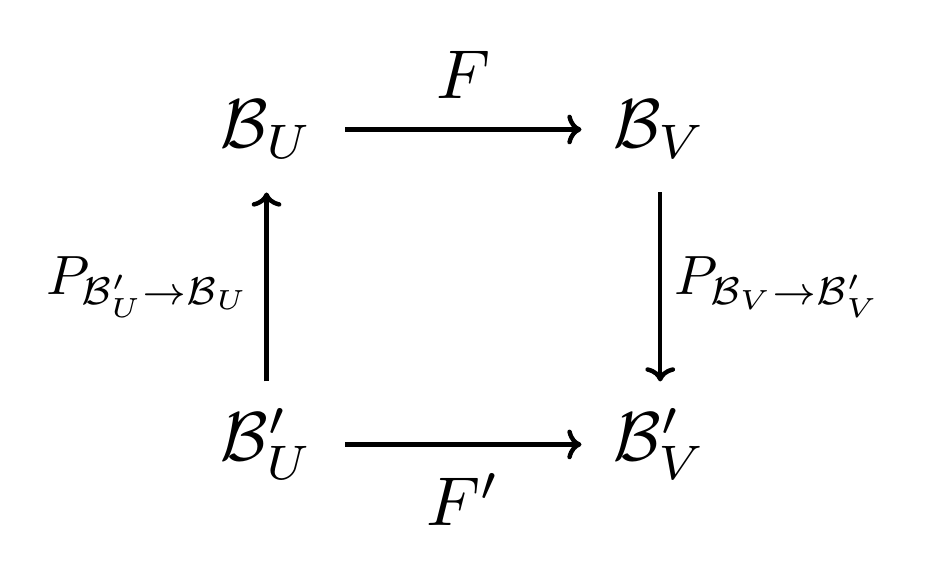
\begin{tikzpicture}
	\coordinate (U)  at (-2.5,+2);
	\coordinate (Ud) at (-2.5,-2);
	\coordinate (V)  at (+2.5,+2);
	\coordinate (Vd) at (+2.5,-2);
	
	\coordinate (F)  at (+0,+2.7);
	\coordinate (Fd) at (+0,-2.7);
	\coordinate (P1) at (-4,+0);
	\coordinate (P2) at (+4,+0);
	
	\node[black,scale=2.5] at (U)  {$\mathcal{B}_U$};
	\node[black,scale=2.5] at (Ud) {$\mathcal{B}'_U$};
	\node[black,scale=2.5] at (V)  {$\mathcal{B}_V$};
	\node[black,scale=2.5] at (Vd) {$\mathcal{B}'_V$};
	
	\node[black,scale=2.5] at (F)  {$F$};
	\node[black,scale=2.5] at (Fd) {$F'$};
	\node[black,scale=2] at (P1) {$P_{\mathcal{B}'_U\to\mathcal{B}_U}$};
	\node[black,scale=2] at (P2) {$P_{\mathcal{B}_V\to\mathcal{B}_V'}$};
	
	\draw[->,ultra thick] ($(U)+(1,0)$)--($(V)-(1,0)$);
	\draw[->,ultra thick] ($(Ud)+(1,0)$)--($(Vd)-(1,0)$);
	\draw[->,ultra thick] ($(Ud)+(0,0.8)$)--($(U)-(0,0.8)$);
	\draw[->,ultra thick] ($(V)-(0,0.8)$)--($(Vd)+(0,0.8)$);
\end{tikzpicture}
\end{figure}
To read this schematic, consider that the arrow for $F'$ has the same input and output as following the other three arrows to go up, then right (through $F$) then down again. This ordered path is the matrix multiplication given above.
}

%\chapter{Eigenvalues and Eigenvectors} \label{ch:eigens}


\definition{Eigenvalues and eigenvectors of a linear map}{
Consider an endomorphism $f:V \to V$ and a vector $\mathbf{v}\in V$. We call a number $\lambda \neq 0$ an eigenvalue of $f$ if there exists a non-zero vector $\mathbf{v}$ satisfying the relation
\begin{align*}
f(\mathbf{v}) = \lambda \mathbf{v}.
\end{align*}
We say that $\mathbf{v}$ is an eigenvector of $f$ \textit{corresponding} or \textit{associated} to the eigenvalue $\lambda$.
}


\definition{Eigenvectors and eigenvalues of a matrix}{
For a square matrix $A$, an eigenvector of $A$ is a non-zero vector, $\mathbf{v}$, that satisfies the matrix equation
\begin{align*}
A\mathbf{v} = \lambda \mathbf{v}
\end{align*}
where $\lambda$ is called an eigenvalue of $A$. We say that $\mathbf{v}$ is an eigenvector of $A$ \textit{corresponding} or \textit{associated} to the eigenvalue $\lambda$.
}


\definition{Characteristic polynomial of a matrix}{
For a square matrix $A$, the \textit{characteristic polynomial} is the given by
\begin{align*}
P(\lambda) = \det ( A - \lambda I)
\end{align*}
where $I$ is the identity matrix with the same size as $A$ and $\lambda$ is the variable of the polynomial. The degree of this polynomial is always the same as the size of the matrix $A$.
}


\definition{Eigenspectrum}{
The eigenvalues of a square matrix $A$ are roots of the characteristic polynomial of $A$. That is, eigenvalues are solutions of
\begin{align*}
 \det ( A - \lambda I) = 0.
\end{align*} 
There can be multiple distinct eigenvalues of $A$, and are conventionally denoted $\lambda_1$, $\lambda_2$, \dots etc. The set of these eigenvalues, $\{\lambda_1, \, \lambda_2, \dots \}$, is called the \textit{eigenspectrum} of $A$.
}


\definition{Eigenspace}{
For any eigenvalue $\lambda_k$ of an $n \times n$ matrix $A$, the eigenspace corresponding to $\lambda_k$, denoted $E_{\lambda_k}$, is the set of all eigenvectors corresponding to $\lambda_k$. This can be written as the set of linear combinations of linearly independent eigenvectors corresponding to $\lambda_k$:
\begin{gather*}
E_{\lambda_k} = \{ \alpha_1 \mathbf{v}_1 + \cdots + \alpha_m \mathbf{v}_m \, | \, \forall j \, A \mathbf{v}_j = \lambda_k \mathbf{v}_j, \, \alpha_j \in \mathbb{R} \} = \text{SPAN}(\mathbf{v}_1, \cdots, \mathbf{v}_m) \\
\text{for maximum number of eigenvectors such that} \\
\alpha_1 \mathbf{v}_1 + \cdots + \alpha_m \mathbf{v}_m = \mathbf{0} \implies  \alpha_1 =  \alpha_2 = \cdots = \alpha_m = 0.
\end{gather*}
As the set $\{\mathbf{v}_1, \cdots, \mathbf{v}_m\}$ generates $E_{\lambda_k}$ and the vectors are linearly independent, the set forms a basis and therefore gives the dimension $E_{\lambda_k}$.

The eigenspace can also be written like a \textit{kernel}
\begin{align*}
E_{\lambda_k} = \{ \mathbf{v} \in \mathbb{R}^n \, | \, \left( A - \lambda_k I \right) \mathbf{v}= \mathbf{0} \}.
\end{align*}
}


\definition{Algebraic and geometric multiplicity of an eigenvalue}{
For an $n \times n$ matrix with characteristic polynomial
\begin{align*}
P(\lambda) = C(\lambda - \lambda_1)^{m_1} \times \cdot \times (\lambda - \lambda_k)^{m_k}\times  \cdot \times (\lambda - \lambda_p)^{m_p}
\end{align*}
for some constant $C$. There can be up to $n$ distinct eigenvalues ($p \leq n$). The exponent $m_k$ is called the \textit{algebraic} multiplicity of the eigenvalue $\lambda_k$. The \textit{dimension} of the eigenspace corresponding to $\lambda_k$ is its \textit{geometric} multiplicity.
}



\definition{Eigenbasis}{
Consider a square matrix $A$ of size $n$. If the dimensions of its eigenspaces add up to $n$, then there exist $n$ linearly independent eigenvectors of $A$. These eigenvectors form a basis of $\mathbb{R}^n$ called an \textit{eigenbasis}.
}


\definition{Similar matrices}{
Two matrices $A$ and $B$ are similar if there exists an invertible matrix $P$ such that
\begin{align*}
B = P A P^{-1}.
\end{align*}
}


\definition{Diagonalizable linear map}{
Let $f:V\to V$ be an endomorphism. $f$ is called \textit{diagonalizable} if there exists a basis, $\mathcal{B}$, of $V$ such that the matrix representation of $f$ in $\mathcal{B}$ is diagonal:
\begin{align*}
(\mathcal{M}(f,\mathcal{B}))_{ij} = 0 \quad \text{whenever } \, i \neq j.
\end{align*}
}

\definition{Diagonalizable matrix}{
A square matrix $A$ is \textit{diagonalizable} if and only if there exists an invertible matrix $P$ and diagonal matrix $D$ such that
\begin{align*}
A = P D P^{-1}.
\end{align*}
Alternative: A square matrix $A$ is \textit{diagonalizable} if and only if it is \textit{similar} to a diagonal matrix $D$. 
}

\definition{Eigenvalue diagonalization}{
For a diagonalizable matrix $A$ of size $n$, we can sometimes find a diagonal matrix consisting of the eigenvalues of $A$, $\lambda_1, \, \dots, \, \lambda_n$. In this case we can write
\begin{align*}
A = P D P^{-1}
\end{align*}
where $P$ consists of eigenvectors of $A$ as columns. The matrix $P$ is the transition matrix from the eigenbasis, $\mathcal{E}$, to the canonical basis of $\mathbb{R}^n$: $P_{\mathcal{E}\to \mathcal{C}_n}$.
}

%\chapter{Inner product spaces} \label{ch:innerproducts}




\definition{Inner product}{
An inner product is a mapping that takes any two vectors of a vector space, $V$, to a scalar, $f:~V\times~V~\to~\mathbb{R}$ but often denoted with angle brackets $f(\mathbf{u},\mathbf{v})=\langle \mathbf{u},\mathbf{v} \rangle$, satisfying the following properties:
\begin{align*}
& \forall \, \mathbf{u},\, \mathbf{v}, \, \mathbf{w} \in V \quad \text{and} \quad  \forall \, k \in \mathbb{R} & \\
(IP1) & \quad \langle \mathbf{u},\mathbf{v} \rangle = \langle \mathbf{v},\mathbf{u} \rangle & (\text{commutativity}) \\
%
(IP2) & \quad \langle \mathbf{u},\mathbf{v}+\mathbf{w} \rangle = \langle \mathbf{u},\mathbf{v} \rangle + \langle \mathbf{u},\mathbf{w} \rangle & (\text{linearity over vector addition}) \\
%
(IP3) & \quad \langle k\mathbf{u},\mathbf{v} \rangle = k\langle \mathbf{u},\mathbf{v} \rangle & (\text{linearity over scalar multiplication}) \\
%
(IP4) & \quad \langle \mathbf{u},\mathbf{u} \rangle \geq 0 & (\text{positive definite})
\end{align*}
}

\definition{Euclidean dot product}{
The \textit{Euclidean dot product} is the canonical inner product defined on the vector space of real $n$-tuples, $\mathbb{R}^n$. Given two vectors $\mathbf{u}=(u_1, \dots, u_n)$ and $\mathbf{v}=(v_1, \dots, v_n)$, their dot product is defined by
\begin{align*}
\mathbf{u} \cdot \mathbf{v} = u_1 v_1 + \cdots + u_n v_n = \sum_{i=1}^n u_i v_i.
\end{align*}
}

\definition{Inner product of functions}{
Let $\mathcal{C}([a,b])$ be the vector space of real functions that are continuous on the interval $[a,b]$. We can define an inner product on any functions $f,g \in \mathcal{C}([a,b])$
\begin{align*}
\langle f,g \rangle = \int_a^b f(x)g(x) dx.
\end{align*}
You should verify that this definition satisfies the 4 properties of inner products.
}

\definition{Inner product space}{
An \textit{inner product space} is a vector space and a definition of an inner product considered as a pair $(V,\langle,\rangle)$. We say that $V$ is \textit{equipped} with the inner product.
}

\definition{Euclidean inner product space}{
A \textit{Euclidean inner product space} is the vector space of real $n$-tuples equipped with the euclidean dot product: $(\mathbb{R}^n, \cdot)$.
}

\definition{Orthogonal vectors}{
Two vectors $\mathbf{u}$ and $\mathbf{v}$ of an inner product space $(V,\langle,\rangle)$ are \textit{orthogonal} if and only if their inner product is zero: $\langle \mathbf{u},\mathbf{v} \rangle = 0$.
}

\definition{Norm}{
A vector $\mathbf{v}$ in an inner product space $(V,\langle,\rangle)$ has \textit{norm}
\begin{align*}
\lVert \mathbf{v} \rVert = \sqrt{\langle \mathbf{v},\mathbf{v} \rangle}.
\end{align*}
The Euclidean norm is therefore
\begin{align*}
\lVert (v_1, \dots, v_n) \rVert = \sqrt{v_1^2 + \cdots + v_n^2}.
\end{align*}
If a vector has norm equal to 1 we say it is a \textit{unit vector} or has \textit{unit length}. If we divide a vector by its norm we say that is has been \textit{normalised}.
}

\definition{To normalise a vector}{
Consider a vector $\mathbf{v}$ in an inner product space $(V,\langle,\rangle)$. We say we ``normalise'' this vector by dividing it by its norm. That is, $\mathbf{v}'$ is the normalised $\mathbf{v}$ if
\begin{align*}
\mathbf{v}' = \frac{\mathbf{v}}{\lVert \mathbf{v} \rVert}.
\end{align*}
}

\noindent When we normalise a vector we guarantee that it has length 1:
\begin{align*}
\lVert  \frac{\mathbf{v}}{\lVert \mathbf{v} \rVert} \rVert =  \frac{\lVert \mathbf{v} \rVert}{\lVert \mathbf{v} \rVert} = 1
\end{align*}


\definition{Orthonormal basis}{
An \textit{orthonormal basis} of an inner product space $(V,\langle,\rangle)$ is a set of vectors 
$\mathcal{B} = \{\mathbf{v}_1, \dots, \mathbf{v}_n\}$ each having norm of 1 and that are pairwise orthogonal:
\begin{align*}
\langle \mathbf{v}_i, \mathbf{v}_j \rangle 
=  
\begin{cases}
1 & \text{whenever } \, i = j, \\
0 & \text{whenever } \, i \neq j.
\end{cases}
\end{align*}
}

%\input{Defs_Diagonalisation.tex}
%\input{Defs_ComplexNumbers.tex}
%\input{Defs_QuantumMechanics.tex}

% List of Definitions and Theorems
%\listoftheorems
%\listoftheorems[ignoreall,show=definition]

%\appendix
%\chapter{Linear Systems} \label{ch:linearsystems}


\section{Basic definitions}

\definition{Linear system of equations}{
A system of $m$ linear equations with $n$ unknowns, denoted $(S)$, has the general form
\begin{align*}
\begin{cases}
a_{11} x_1  + a_{12} x_2 + \cdots + a_{1n} x_n = y_1 \\
a_{21} x_1  + a_{22} x_2 + \cdots + a_{2n} x_n = y_2 \\
\vdots \\
a_{m1} x_1  + a_{m2} x_2 + \cdots + a_{mn} x_n = y_m
\end{cases}
\qquad (S)
\end{align*}
where the $x_j$ are the unknowns we want to find, $a_{ij}$ are the \textit{coefficients} and  the $y_i$ are the \textit{constant terms}.
}

We group the coefficients into a matrix $A=(a_{ij})$, the unknowns and constants into columns $X$ and $Y$ so that the system can be written as a matrix equation $AX=Y$. 

\begin{align*}
\underbrace{
\begin{pmatrix}
a_{11} & a_{12} & \cdots & a_{1n} \\
a_{21} & a_{22} & \cdots & a_{2n} \\
\vdots & \vdots & \ddots & \vdots \\
a_{m1} & a_{m2} & \cdots & a_{mn}
\end{pmatrix}}_A
%%
%%
\underbrace{
\begin{pmatrix}
x_{1} \\
x_{2} \\
\vdots \\
x_{n}
\end{pmatrix}}_X
%%
=
\underbrace{
\begin{pmatrix}
y_{1} \\
y_{2} \\
\vdots \\
y_{m}
\end{pmatrix}}_Y
\end{align*}

The goal is to find all the possible collections of $x_i$, called a \textit{solution}, that satisfy the equation $AX=Y$. That is, the possible columns $X$. We denote the set of solutions of $(S)$ as $\mathcal{S}$, which is a subset of all columns of size $n$.

Note: it is possible that $\mathcal{S}$ is an empty set, which would mean there are no solutions of $AX=Y$. For example, if two parallel lines are offset by some distance, there is no point of intersection.

\example{A solution of a linear system of two equations and three unknowns}{
For a system
\begin{align*}
\underbrace{
\begin{pmatrix}
1 & 2 & 3 \\
2 & 0 & 1
\end{pmatrix}}_A
%%
%%
\underbrace{
\begin{pmatrix}
x_{1} \\
x_{2} \\
x_{3}
\end{pmatrix}}_X
%%
=
\underbrace{
\begin{pmatrix}
1 \\
2
\end{pmatrix}}_Y
\qquad (S)
\end{align*}
Since
\begin{align*}
\begin{pmatrix}
1 & 2 & 3 \\
2 & 0 & 1
\end{pmatrix}
%%
%%
\begin{pmatrix}
-1 \\
-5 \\
4
\end{pmatrix}
%%
=
\begin{pmatrix}
1 \\
2
\end{pmatrix}
%
\quad\text{and}\quad
%
\begin{pmatrix}
1 & 2 & 3 \\
2 & 0 & 1
\end{pmatrix}
%%
%%
\begin{pmatrix}
-3 \\
-10 \\
8
\end{pmatrix}
%%
=
\begin{pmatrix}
1 \\
2
\end{pmatrix}
\end{align*}
then $(x_1,x_2,x_3)=(-1,-5,4)$ and $(x_1,x_2,x_3)=(-3,-10,8)$ are two solutions of $(S)$.
}

\definition{Homogeneous linear system}{
For any system of linear equations, $(S)$, given by $AX=Y$, we associate the \textbf{homogeneous system}, denoted $(H)$:
\begin{align*}
 AX = 0_m
\end{align*} 
for the column
\begin{align*}
0_m = \begin{pmatrix} 0 \\ 0 \\ \vdots \\ 0 \end{pmatrix} \in \mathcal{M}_{m,1}
\end{align*}
We will denote the solution set of $(H)$ by $\mathcal{H}$.

Note: the homogeneous system always admits \textit{at least one} solution, the trivial solution $X=0_n$.
}


\section{Properties of solutions of linear systems}

\theorem{Scalar multiples of homogeneous solutions}{
If $X$ is a solution of $(H)$, then any scalar multiple of $X$ is also a solution of $(H)$.
}
\begin{proof}
Let $AX=0_m$ and $k\in\mathbb{R}$. Then
\begin{align*}
A(kX) &= k(AX) \\
&=k0_m \\
&=0_m 
\end{align*}
Therefore $kX$ is a solution of $(H)$.
\end{proof}


\example{Homogeneous solutions}{
For a system
\begin{align*}
\underbrace{
\begin{pmatrix}
1 &  1 & 1 \\
2 & -1 & 0
\end{pmatrix}}_A
%%
%%
\underbrace{
\begin{pmatrix}
x_{1} \\
x_{2} \\
x_{3}
\end{pmatrix}}_X
%%
=
\underbrace{
\begin{pmatrix}
0 \\
0
\end{pmatrix}}_Y
%%
\qquad \text{and} \qquad
%%
\begin{pmatrix}
1 &  1 & 1 \\
2 & -1 & 0
\end{pmatrix}
%%
%%
\begin{pmatrix}
1 \\
2 \\
-3
\end{pmatrix}
%%
=
\begin{pmatrix}
0 \\
0
\end{pmatrix}
\end{align*}
we have $(x_1,x_2,x_3)=(1,2,-3)$ as a solution. Let's check $\pi$ times this column
\begin{align*}
\begin{pmatrix}
1 &  1 & 1 \\
2 & -1 & 0
\end{pmatrix}
%%
%%
\begin{pmatrix}
\pi \\
2\pi \\
-3\pi
\end{pmatrix}
%%
=
\begin{pmatrix}
\pi + 2\pi - 3\pi \\
2\pi - 2\pi
\end{pmatrix}
%%
=
\begin{pmatrix}
0 \\
0
\end{pmatrix}
\end{align*}
So $(x_1,x_2,x_3)=(\pi,2\pi,-3\pi)$ is also a solution.
}

\theorem{Addition of homogeneous solutions}{
If $X$ and $X'$ are solutions of $(H)$, then their addition $X+X'$ is also a solution of $(H)$.}

\begin{proof}
Let $AX=0_m$ and $AX'=0_m$. Then
\begin{align*}
A(X + X') &= AX + AX' & \text{(distributivity)} \\
&=0_m + 0_m & \text{(using the premise)}\\
&=0_m & \text{(definition of zero matrix)}
\end{align*}
Therefore $X+X'$ is a solution of $(H)$.
\end{proof}

\theorem{Trivial or infinite homogeneous solutions}{
Homogeneous linear systems have either only the trivial solution (zero column) or infinite solutions.
} 

In effect, if the system $(H)$ has a non-zero solution $X$, then all columns of the form $kX$ for $k\in\mathbb{R}$ are distinct solutions of $(H)$, and there are infinitely many of them.

\theorem{Solution set of a system}{
For any system $(S)$, if it has at least one solution, call it $X_p$, then the set of solutions can be written
\begin{align*}
\mathcal{S} = \left\{ X_p + X_h \, | \, \forall X_h \in \mathcal{H} \right\}
\end{align*}
where $\mathcal{H}$ is the set of solutions of the associated homogeneous system of $(S)$.
}

\begin{proof} 
Let $X_p$ be any solution of the system $AX=Y$ and $X_h$ be any solution of the associated homogeneous system. Then we have
\begin{align*}
A(X_p + X_h) &= \underbrace{AX_p}_Y + \underbrace{AX_h}_{0_m} = Y + 0_m = Y
\end{align*}
Hence $X_p + X_h$ is also a solution of $AX=Y$.
\end{proof}


\theorem{Number of solutions of a system}{
Any system, $(S)$, has either
\begin{itemize}
\item no solutions,
\item 1 unique solution,
\item infinite solutions.
\end{itemize}
}

This follows immediately from the previous two theorems.

\theorem{Solution with inverse}{
Let $A$ be a given square matrix and $(S)$ be the system $AX=Y$. If $A$ is invertible, then $(S)$ has 1 unique solution given by
\begin{align*}
X = A^{-1} Y.
\end{align*}
}

\begin{proof}
\noindent \underline{Is $A^{-1}Y$ a solution to $AX=Y$?}
\begin{align*}
A(A^{-1}Y) &= (AA^{-1})Y \\
 &= IY \\
 &= Y
\end{align*}
Yes.

\noindent \underline{Is $A^{-1}Y$ unique?}

Let $X_p$ be some solution of $AX=Y$. Then
\begin{align*}
 AX_p &= Y \\
 A^{-1} AX_p &= A^{-1}Y \\
 IX_p &= A^{-1}Y \\
 X_p &= A^{-1}Y
\end{align*}
Yes.

\end{proof}



\theorem{System with inverse}{
Let $A$ be a square matrix. If the system of equations, $(S)$, represented by $AX = Y$ has a solution for every possible $Y$, then $A$ is invertible.
}

\theorem{Invertible linear systems have unique solutions.}{
Let $A$ be an invertible square matrix. For any two columns $X$ and $X'$ satisfying $AX=AX'$, we then have $X=X'$.
}

\begin{proof}
\begin{gather*}
AX = AX' \\
A^{-1}AX = A^{-1}AX' \\
IX = IX' \\
X = X'
\end{gather*}
\end{proof}



\section{Gaussian reduction}

\definition{Equivalent systems}{
Two systems of linear equations are \textbf{equivalent} if they share the same set of solutions.
}

\example{Equivalent systems}{

\begin{align*}
(S_1)
\begin{cases}
    I_1 +   I_2 -   I_3 =  0 \\
 13 I_1 - 6 I_2         = 20 \\
          6 I_2 + 8 I_3 = 30
\end{cases}
\quad\text{and}\quad
(S_2)
\begin{cases}
    I_1 +   I_2 -   I_3 =  0 \\
          6 I_2 + 8 I_3 = 30 \\
 13 I_1 - 6 I_2         = 20 
\end{cases}
\end{align*}

$(S_2)$ is simply a reordering of the equations of $(S_1)$, so it obviously has the same solution, $(I_1, I_2, I_3) = (3,2,1)$. Hence $(S_1)$ and $(S_2)$ are equivalent systems.
}

\definition{Elementary operations}{

There are \textbf{elementary operations} that we can do to systems of equations that give new systems that remain equivalent to the old.

\centering

\underline{Exchanging two equations} \vspace{-0.4cm}
\begin{align*}
(S_1)
\begin{cases}
    I_1 +   I_2 -   I_3 =  0 \\
 13 I_1 - 6 I_2         = 20 
\end{cases}
\quad\equiv\quad
(S_2)
\begin{cases}
 13 I_1 - 6 I_2         = 20 \\
    I_1 +   I_2 -   I_3 =  0 
\end{cases}
\end{align*}
\underline{Multiplying one equation by a non-zero constant} \vspace{-0.4cm}
\begin{align*}
(S_1)
\begin{cases}
    I_1 +   I_2 -   I_3 =  0 \\
 13 I_1 - 6 I_2         = 20 
\end{cases}
\quad\equiv\quad
(S_2)
\begin{cases}
    I_1 +   I_2 -   I_3 =  0 \\
 I_1 - (6/13) I_2         = (20/13) 
\end{cases}
\end{align*}
\underline{Adding a multiple of one equation to another equation} \vspace{-0.4cm}
\begin{align*}
(S_1)
\begin{cases}
    I_1 +   I_2 -   I_3 =  0 \\
 13 I_1 - 6 I_2         = 20 
\end{cases}
\quad\equiv\quad
(S_2)
\begin{cases}
    I_1 +   I_2 -   I_3 =  0 \\
 15 I_1 - 4 I_2 - 2 I_3 = 20 
\end{cases}
\end{align*}
}

These elementary operations will be used in a method to solve systems of equations, called \textbf{Gaussian reduction}. Before summarising the algorithm, we'll use it on a concrete example. Consider the system of linear equations with unknowns $x$, $y$, $z$, and $t$:
\begin{align*}
(S_1)
\left\{
\begin{matrix}
    x &+  3y &-  z &+  4t &=&   27 \\
  -4x &- 11y &+ 6z &- 14t &=& -105 \\
  -2x &- 10y &- 7z &- 14t &=&  -55 \\
   2x &+  9y &+ 6z &+  9t &=&   37
\end{matrix}
\right.
\end{align*}
The solution set, $\mathcal{S}$, is clearly a subset of $\mathbb{R}^4$, that is, a set of quadruples. We can rewrite $(S_1)$ in matrix form
\begin{align*}
\underbrace{
\begin{pmatrix}
   1 &   3 & -1 &   4 \\
  -4 & -11 &  6 & -14 \\
  -2 & -10 & -7 & -14 \\
   2 &   9 &  6 &   9
\end{pmatrix}}_A
%%
%%
\underbrace{
\begin{pmatrix}
x \\
y \\
z \\
t
\end{pmatrix}}_X
%%
=
\underbrace{
\begin{pmatrix}
27 \\
-105 \\
-55 \\
37
\end{pmatrix}}_Y
\end{align*}
We will solve this system using the Gaussian reduction. First keeping it in equation form, and then in shorthand with the matrix representation.

The general goal is to use the elementary operations to simplify the equations, so that there are ``leading 1s'', called pivots. The pivots are used to eliminate unknowns in different equations. Let's denote the lines as $L_i$ and the notation, for example, $L_1 \to L_1 + 2L_2$ will mean that we add 2 times line 2 to line 1. Now, our system already has a pivot for the first equation
\begin{align*}
(S_2)
\left\{
\begin{matrix}
   \colourboxed{airforceblue}{1}x &+  3y &-  z &+  4t &=&   27 \\
  -4x & -11y & +6z & -14t &=& -105 \\
  -2x & -10y & -7z & -14t &=&  -55 \\
   2x & + 9y & +6z & + 9t &=&   37
\end{matrix}
\right.
\end{align*}
We use this pivot to eliminate the unknown $x$ from the other 3 equations. For the 2nd
line, add 4 of the 1st. Add 2 of the 1st to the 3rd . Add -2 of the first to the 4th.
\begin{align*}
(S_3)
\left\{
\begin{matrix}
   \colourboxed{airforceblue}{1}x & +3y &-  z & +4t &=&   27 & \\
   0  & +1y & +2z & +2t &=&    3 & L_2 \to L_2 + 4L_1\\
   0  & -4y & -9z & -6t &=&   -1 & L_3 \to L_3 + 2L_1\\
   0  & +3y & +8z & + t &=&  -17 & L_4 \to L_4 - 2L_1
\end{matrix}
\right.
\end{align*}
We now use the pivot in the second equation to eliminate the unknown $x$ from the
lower 2 equations. For the 3nd line, add 4 of the 2nd. Subtract 3 of the 2nd to the 4th.
\begin{align*}
(S_4)
\left\{
\begin{matrix}
   x & +3y &-  z & +4t &=&   27 & \\
   0  & \colourboxed{airforceblue}{1}y & +2z & +2t &=& 3 & \\
   0  & 0 & -1z & +2t &=&  11 & L_3 \to L_3 + 4L_2\\
   0  & 0 & +2z & -5t &=& -26 & L_4 \to L_4 - 3L_2
\end{matrix}
\right.
\end{align*}
We now use the new pivot ($-1$ is as good as 1) in the third equation to eliminate the
unknown $x$ from the fourth equation. So, add 2 of the 3rd to the 4th.
\begin{align*}
(S_5)
\left\{
\begin{matrix}
   x & +3y &-  z & +4t &=&   27 & \\
   0  & y & +2z & +2t &=& 3 & \\
   0  & 0 & \colourboxed{airforceblue}{-1}z & +2t &=&  11 & \\
   0  & 0 & 0 & -t &=& -4 & L_4 \to L_4 + 3L_3
\end{matrix}
\right.
\end{align*}
As we have used elementary operations in going from $(S_1) \to (S_2) \to \dots \to (S_5)$, all of these systems are equivalent to each other. Hence the set of solutions of $(S_5)$ is the same as for $(S_1)$, which we originally seek. This final form of the equations lets us give a quadruple of numbers, the solution to $(S_1)$:
\begin{align*}
(S_5)
&\left\{
\begin{matrix}
   x & +3y & -z & +4t &=& 27 \\
   0  & y & +2z & +2t &=& 3 \\
   0  & 0 & -z & +2t &=&  11 \\
   0  & 0 & 0 & -t &=& -4
\end{matrix}
\right. \\
(S_5)
&\left\{
\begin{array}{ll}
   t &= 4 \\
   z &= 2t -  11 = -3\\
   y &= 3 -2z - 2t = 1\\
   x &= 27 - 3y + z - 4t = 5 	
\end{array}
\right. 
\end{align*}
So we have a solution to the system $(S_1)$: $(x,y,z,t)=(5,1,-3,4)$. And the set of solutions contains just this one, unique solution: $\mathcal{S}=\{(5,1,-3,4)\}$. \textit{Note}: The set $\mathcal{S}$ is a set of 4-tuples (in this case just 1), and not a set of 4 separate numbers.


\subsection*{Gaussian reduction in matrix form}

Consider the almost-same system of linear equations with different constant terms
\begin{align*}
(S)
\left\{
\begin{matrix}
    x &+  3y &-  z &+  4t &=&  -10 \\
  -4x &- 11y &+ 6z &- 14t &=&   35 \\
  -2x &- 10y &- 7z &- 14t &=&   29 \\
   2x &+  9y &+ 6z &+  9t &=&   -8
\end{matrix}
\right.
\end{align*}
To shorthand the Gaussian reduction we convert the system into an \textbf{augmented matrix}
\begin{align*}
\left(
	\begin{matrix}
	   1 &   3 & -1 &   4 \\
	  -4 & -11 &  6 & -14 \\
	  -2 & -10 & -7 & -14 \\
	   2 &   9 &  6 &   9
	\end{matrix}
  \left|
	\begin{matrix}
	 -10 \\
	  35 \\
	  29 \\
	  -8
	\end{matrix}
  \right.
\right)
\end{align*}

We can use this representation to make elementary row operations, without having to write down the variables in each line. So we denote rows by $R_i$. The matrix $A$ is the same as the previous example, so the operations will be the same. The constant terms are the only difference between the two examples.

As previously, we use the first row’s pivot to eliminate the unknown $x$ from the other 3 rows. For the 2nd row, add 4 of the 1st. Add 2 of the 1st to the 3rd. Add $-2$ of the first to the 4th.
\begin{align*}
\begin{array}{l}
   \\
 R_2 \to R_2 + 4R_1 \\
 R_3 \to R_3 + 2R_1 \\
 R_4 \to R_4 - 2R_1
\end{array}
\quad
\left(
	\begin{matrix}
	   1 &   3 & -1 &   4 \\
	   0 &   1 &  2 &   2 \\
	   0 &  -4 & -9 &  -6 \\
	   0 &   3 &  8 &   1
	\end{matrix}
  \left|
	\begin{matrix}
	 -10 \\
	  -5 \\
	   9 \\
	  12
	\end{matrix}
  \right.
\right)
\end{align*}
We now use the pivot in the second row to eliminate the unknown $y$ from the lower 2 rows. For the 3nd row, add 4 of the 2nd. Subtract 3 of the 2nd from the 4th.
\begin{align*}
\begin{array}{l}
   \\
   \\
 R_3 \to R_3 + 4R_2 \\
 R_4 \to R_4 - 3R_2
\end{array}
\quad
\left(
	\begin{matrix}
	   1 &   3 & -1 &   4 \\
	   0 &   1 &  2 &   2 \\
	   0 &   0 & -1 &   2 \\
	   0 &   0 &  2 &  -5
	\end{matrix}
  \left|
	\begin{matrix}
	 -10 \\
	  -5 \\
	 -11 \\
	  27
	\end{matrix}
  \right.
\right)
\end{align*}
We now use the new pivot in the third row to eliminate the unknown $z$ from the fourth
row. So, add 2 of the 3rd to the 4th.
\begin{align*}
\begin{array}{l}
   \\
   \\
   \\
 R_4 \to R_4 + 2R_3
\end{array}
\quad
\left(
	\begin{matrix}
	   1 &   3 & -1 &   4 \\
	   0 &   1 &  2 &   2 \\
	   0 &   0 & -1 &   2 \\
	   0 &   0 &  0 &  -1
	\end{matrix}
  \left|
	\begin{matrix}
	 -10 \\
	  -5 \\
	 -11 \\
	   5
	\end{matrix}
  \right.
\right)
\end{align*}
We now ``unpack'' the augmented matrix to see it again as a system of equations
\begin{align*}
\left(
	\begin{matrix}
	   1 &   3 & -1 &   4 \\
	   0 &   1 &  2 &   2 \\
	   0 &   0 & -1 &   2 \\
	   0 &   0 &  0 &  -1
	\end{matrix}
  \left|
	\begin{matrix}
	 -10 \\
	  -5 \\
	 -11 \\
	   5
	\end{matrix}
  \right.
\right)
\longrightarrow
(S')
\left\{
\begin{matrix}
    x &+ 3y &-  z &+ 4t &=&  -10 \\
    0 &+  y &+ 2z &+ 2t &=&   -5 \\
    0 &+  0 &-  z &- 2t &=&  -11 \\
    0 &+  0 &+  0 &-  t &=&    5
\end{matrix}
\right.
\end{align*}
And as before, a little more work to find the solution
\begin{align*}
(S')
&\left\{
\begin{array}{ll}
   t &=  -5 \\
   z &=  2t +11 = 1\\
   y &=  -5 -2z - 2t = 3\\
   x &= -10 -3y + z - 4t = 2 	
\end{array}
\right. 
\end{align*}
So we have a solution to the system $(S)$: $(x,y,z,t)=(2,3,1,-5)$. And the set of solutions contains just this one, unique solution: $\mathcal{S}=\{(2,3,1,-5)\}$.


\subsection*{Inverse matrix from Gaussian reduction}
One more time, let’s consider the same matrix A, but with general constant terms
\begin{align*}
(S)
\left\{
\begin{matrix}
    x &+  3y &-  z &+  4t &=&  a \\
  -4x &- 11y &+ 6z &- 14t &=&  b \\
  -2x &- 10y &- 7z &- 14t &=&  c \\
   2x &+  9y &+ 6z &+  9t &=&  d
\end{matrix}
\right.
\quad
\longrightarrow
\quad
\left(
	\begin{matrix}
	   1 &   3 & -1 &   4 \\
	  -4 & -11 &  6 & -14 \\
	  -2 & -10 & -7 & -14 \\
	   2 &   9 &  6 &   9
	\end{matrix}
  \left|
	\begin{matrix}
	  a \\
	  b \\
	  c \\
	  d
	\end{matrix}
  \right.
\right)
\end{align*}
And we proceed with the exact same row operations as before. Only the constant
terms are different.
\begin{align*}
\begin{array}{l}
   \\
 R_2 + 4R_1 \\
 R_3 + 2R_1 \\
 R_4 - 2R_1
\end{array}
&\quad
\left(
	\begin{matrix}
	   1 &   3 & -1 &   4 \\
	   0 &   1 &  2 &   2 \\
	   0 &  -4 & -9 &  -6 \\
	   0 &   3 &  8 &   1
	\end{matrix}
  \left|
	\begin{matrix}
	  a \\
	  b+4a \\
	  c+2a \\
	  d-2a
	\end{matrix}
  \right.
\right)
%%%%%
%%%%%
%%%%%
\\
%%%%%
%%%%%
%%%%%
\begin{array}{l}
   \\
 \longrightarrow \\
   \\
\end{array}
\begin{array}{l}
  \\
  \\
 R_3 + 4R_2 \\
 R_4 - 3R_2
\end{array}
&\quad
\left(
	\begin{matrix}
	   1 &   3 & -1 &   4 \\
	   0 &   1 &  2 &   2 \\
	   0 &   0 & -1 &   2 \\
	   0 &   0 &  2 &  -5
	\end{matrix}
  \left|
	\begin{matrix}
	  a \\
	  b+4a \\
	  c+18a+4b \\
	  d-14a-3b
	\end{matrix}
  \right.
\right)
%%%%%
%%%%%
%%%%%
\\
%%%%%
%%%%%
%%%%%
\begin{array}{l}
   \\
 \longrightarrow \\
   \\
\end{array}
\begin{array}{l}
   \\
   \\
  \\
 R_4 + 2R_3
\end{array}
&\quad
\left(
	\begin{matrix}
	   1 &   3 & -1 &   4 \\
	   0 &   1 &  2 &   2 \\
	   0 &   0 & -1 &   2 \\
	   0 &   0 &  0 &  -1
	\end{matrix}
  \left|
	\begin{matrix}
	  a \\
	  b+4a \\
	  c+18a+4b \\
	  d+22a+5b+2c
	\end{matrix}
  \right.
\right)
\end{align*}
Unpacking back into equation form
\begin{align*}
(S')
\left\{
\begin{matrix}
    x &+ 3y &-  z &+ 4t &=&  a \\
    0 &+  y &+ 2z &+ 2t &=&  b+4a \\
    0 &+  0 &-  z &- 2t &=&  c+18a+4b \\
    0 &+  0 &+  0 &-  t &=&  d+22a+5b+2c
\end{matrix}
\right.
\end{align*}
Solving for the unknowns
\begin{align*}
\begin{array}{ll}
   t &=  -22a-5b-2c -d\\
   z &=  2t -18a-4b-c  = -62a-14b-5c-2d\\
   y &=  -2z - 2t +4a+b = 172a+39b+14c+6d\\
   x &= -3y + z - 4t + a = -489a - 111b-39c-16d 	
\end{array}
\end{align*}
In order, then, we have the solution
\begin{align*}
&
\begin{array}{rlrrrr}
   x &=& -489a & -111b & -39c & -16d \\
   y &=&  172a &  +39b & +14c &  +6d \\
   z &=&  -62a &  -14b &  -5c &  -2d \\
   t &=&  -22a &   -5b &  -2c &   -d
\end{array}
\\
&
\underbrace{
\begin{pmatrix}
   x \\
   y \\
   z \\
   t
\end{pmatrix}
}_{X}
=
\underbrace{
\begin{pmatrix}
   -489 & -111 & -39 & -16 \\
    172 &   39 &  14 &   6 \\
    -62 &  -14 &  -5 &  -2 \\
    -22 &   -5 &  -2 &  -1
\end{pmatrix}
}_{B}
\underbrace{
\begin{pmatrix}
   a \\
   b \\
   c \\
   d
\end{pmatrix}
}_{Y}
\end{align*}
Writing this out like this allows us to solve $AX=Y$ for any arbitrary 4-tuple $Y$. Recall the theorem that states that this property means $A$ is invertible. \textbf{$B$ is exactly the inverse of $A$}.

\subsection*{Column exchange}
Consider the following system
\begin{align*}
(S)
\left\{
\begin{matrix}
 -11x &  +6y &  -4z & -14t &=& -105 \\
   9x &  +6y &  +2z &  +9t &=&   37 \\
   3x &   -y &   +z &  +4t &=&   27 \\
 -10x &  -7y &  -2z & -14t &=&  -55
\end{matrix}
\right.
\end{align*}
If we wanted to form a pivot in the first line we would have divide this line by $-11$. This is perfectly legitimate, but introduces fractions that will make computations very messy and prone to error later. Instead we could switch lines 1 and 3, and rewrite the equations with $z$ being the leading term:
\begin{align*}
(S')
\left\{
\begin{matrix}
   +z &  3x &   -y &  +4t &=&   27 \\
  +2z &  9x &  +6y &  +9t &=&   37 \\
  -4z &-11x &  +6y & -14t &=& -105 \\
  -2z &-10x &  -7y & -14t &=&  -55
\end{matrix}
\right.
\end{align*}


\begin{align*}
(S')
\left\{
\begin{matrix}
   +z &  3x &   -y &  +4t &=&   27 \\
  +2z &  9x &  +6y &  +9t &=&   37 \\
  -4z &-11x &  +6y & -14t &=& -105 \\
  -2z &-10x &  -7y & -14t &=&  -55
\end{matrix}
\right.
\end{align*}
But be careful, when solving this system using augmented matrix form you must remember that the first column now refers to the $z$ variable. So when you find the solution, you should put it into the original order of unknowns $(x,y,z,t)$:
\begin{align*}
\mathcal{S} = \{(1,-3,5,4) \}
\end{align*}


\example{A system with no solutions}{
\begin{align*}
&
\left(
	\begin{matrix}
	   1 &   3 &  -1 &   4 \\
	  -4 & -11 &   6 & -14 \\
	  -2 & -10 &  -7 & -14 \\
	   1 &   3 &  -1 &   4
	\end{matrix}
  \left|
	\begin{matrix}
	    27 \\
	  -105 \\
	   -55 \\
	  2015
	\end{matrix}
  \right.
\right) \\
&
\begin{array}{l}
   \\
 R_2 + 4R_1 \\
 R_3 + 2R_1 \\
 R_4 - 1R_1
\end{array}
\,
\left(
	\begin{matrix}
	   1 &   3 &  -1 &   4 \\
	   0 &   1 &   2 &   2 \\
	   0 &  -4 &  -9 &  -6 \\
	   0 &   0 &   0 &   0
	\end{matrix}
  \left|
	\begin{matrix}
	    27 \\
	     3 \\
	    -1 \\
	  1988
	\end{matrix}
  \right.
\right)
\end{align*}
The last row gives the absurd equation $0x + 0y + 0z + 0t = 1998$. And so this system of equations is insoluble.

\noindent \textit{The lesson}: if any 2 rows of $A$ are the same (assuming the constant terms are different), the system has no solutions.
}

\subsection*{Types of systems}

\example{A system with infinite solutions}{

\begin{align*}
(S)
\left\{
\begin{matrix}
    x &  +3y &   -z &  +4t &=&   27 \\
  -4x & -11y &  +6z & -14t &=& -105 \\
  -2x & -10y &  -7z & -14t &=&  -55 \\
    x &  +3y &   -z &  +4t &=&   27
\end{matrix}
\right.
\end{align*}
In this system, the 4th equation is identical to the 3rd. So it really reduces down
to 3 independent equations.
\begin{align*}
(S_1)
\left\{
\begin{matrix}
    x &  +3y &   -z &  +4t &=&   27 \\
  -4x & -11y &  +6z & -14t &=& -105 \\
  -2x & -10y &  -7z & -14t &=&  -55
\end{matrix}
\right.
\end{align*}
}

\example{A system with infinite solutions}{
\begin{align*}
&
(S_2)
\left\{
\begin{matrix}
    x &  +3y &   -z &  +4t &=&   27 \\
    0 &    y &  +2z &  +2t &=&    3 \\
    0 &  -4y &  -9z &  -6t &=&   -1
\end{matrix}
\right.
\quad
\begin{array}{l}
   \\
 L_2 + 4L_1 \\
 L_3 + 2L_1
\end{array}
\\
&
(S_2)
\left\{
\begin{matrix}
    x &  +3y &   -z &  +4t &=&   27 \\
    0 &    y &  +2z &  +2t &=&    3 \\
    0 &    0 &   -z &  +2t &=&   11
\end{matrix}
\right.
\quad
\begin{array}{l}
   \\
   \\
 L_3 + 4L_2
\end{array}
\end{align*}
This is as far as we can go. $t$ is a \textbf{free variable}, i.e. arbitrary, and the other unknowns can be rewritten entirely in terms of it. Working from the last equation first:
\begin{align*}
\begin{array}{ll}
   z &=  2t -11\\
   y &=  3 -2z - 2t = -6t + 25\\
   x &= 27 - 3y + z - 4t = 16t - 59
\end{array}
\end{align*}

There is a different set of 4 numbers for each $t$, i.e. there are infinite 4-tuples that solve  $(S)$. They can be be written in column form
\begin{align*}
\begin{pmatrix}
   x \\
   y \\
   z \\
   t
\end{pmatrix}
=
\begin{pmatrix}
   16t - 59 \\
   -6t + 25\\
    2t - 11\\
     t
\end{pmatrix}
=
\begin{pmatrix}
   16 \\
    -6 \\
   2\\
   1
\end{pmatrix}
t
+
\begin{pmatrix}
   -59 \\
    25 \\
   -11 \\
     0
\end{pmatrix}
\end{align*}
Or as the set of solutions
\begin{align*}
\mathcal{S} = \{ (16,-6,2,1)t + (-59,25,-11,0) \, | \, \forall	t\in\mathbb{R} \}
\end{align*}
The column form of the solution allows for a nice geometric interpretation of the solution space
\begin{align*}
\begin{pmatrix}
   x \\
   y \\
   z \\
   t
\end{pmatrix}
=
\begin{pmatrix}
   16t - 59 \\
   -6t + 25\\
    2t - 11\\
     t
\end{pmatrix}
=
\begin{pmatrix}
   16 \\
    -6 \\
   2\\
   1
\end{pmatrix}
t
+
\begin{pmatrix}
   -59 \\
    25 \\
   -11 \\
     0
\end{pmatrix}
\end{align*}
\begin{center}
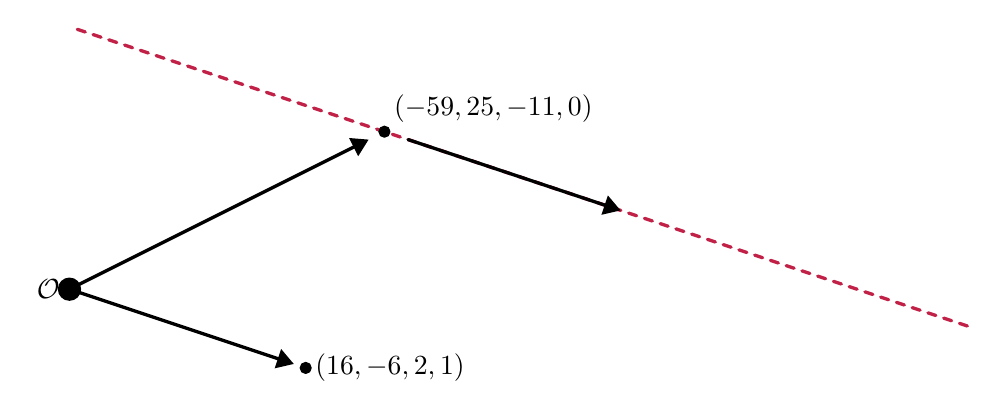
\begin{tikzpicture}[line cap=round, line join=round, >=Triangle,scale=2]
	% coordinate system
	\coordinate (O) at (0,0); 
	\coordinate (A) at (2,1); 
	\coordinate (B) at (1.5,-0.5); 
	
	% straight lines y= x/2 + 1, y=x/3 + 1 and y= -x/3 + 2
	\draw[->,very thick,black] (O)--($(O)+0.95*(A)$);
	\draw[->,very thick,black] (O)--($0.95*(B)$);
	\draw[dashed,very thick,brightmaroon] ($(A)-1.3*(B)$)--($(A)+2.5*(B)$);
	\draw[->,very thick,black] ($(A)+0.1*(B)$)--($(A)+(B)$);
	\filldraw [black] (O) circle (2pt) node[left] {$\mathcal{O}$};
	\filldraw [black] (B) circle (1pt) node[right] {$(16,-6,2,1)$};
	\filldraw [black] (A) circle (1pt) node[above right] {$(-59,25,-11,0)$};

\end{tikzpicture}
\end{center}

All the points on the red dashed line are solutions of $AX=Y$.
}



\definition{Overdetermined system}{
An overdetermined system has more equations than unknowns. We say “there are too many equations”. Such a system allows solutions only if certain conditions are met. 
}

\noindent For example, in the following figure we have 3 straight lines.

\begin{center}
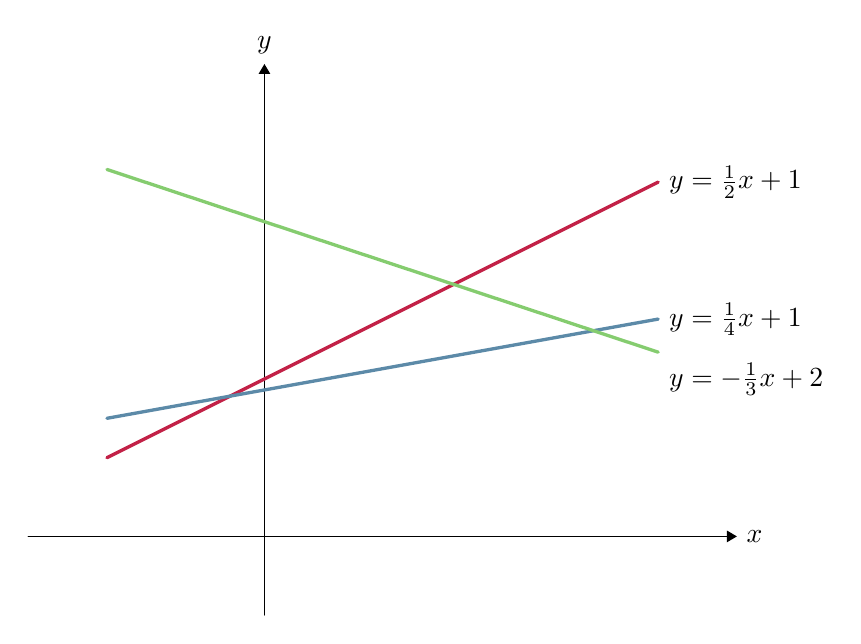
\begin{tikzpicture}[line cap=round, line join=round, >=Triangle,scale=2]
	% coordinate system
	\coordinate (O) at (0,0); 
	\draw[->] (-1.5, 0) -- (3,0) node[right] {$x$};
	\draw[->] (0, -0.5) -- (0,3) node[above] {$y$};
	
	% straight lines y= x/2 + 1, y=x/3 + 1 and y= -x/3 + 2
	\draw[-,very thick,brightmaroon] (-1,0.5)--(2.5,2.25) node[right,black] {$y= \frac{1}{2}x + 1$};
	\draw[-,very thick,airforceblue] (-1,0.75)--(2.5,1.38) node[right,black] {$y=\frac{1}{4}x + 1$};
	\draw[-,very thick,nicegreen] (-1,2.33)--(2.5,1.17) node[below right,black] {$y= -\frac{1}{3}x + 2$};

\end{tikzpicture}
\end{center}
There is nowhere that all three of these lines overlap, that is, nowhere that the three equations are simultaneously true.



\example{Overdetermined system with one solution}{
The following overdetermined system, despite have 5 equations and 4 unknowns, has exactly one solution
\begin{align*}
(S)
\left\{
\begin{matrix}
    x &  +3y &   -z &  +4t &=&   27 \\
  -4x & -11y &  +6z & -14t &=& -105 \\
  -2x & -10y &  -7z & -14t &=&  -55 \\
   2x &  +9y &  +6z &  +9t &=&   37 \\
   2x & +18y & +26z & +23t &=&   42
\end{matrix}
\right.
\end{align*}
After many lines of the usual Gaussian method, we arrive at \hspace{-0.3cm}
\begin{align*}
\left(
	\begin{matrix}
	   1 &   3 &  -1 &   4 \\
	   0 &   1 &   2 &   2 \\
	   0 &   0 &  -1 &   2 \\
	   0 &   0 &   0 & -1 \\
	   0 &   0 &   0 & -1
	\end{matrix}
  \left|
	\begin{matrix}
	    27 \\
	     3 \\
	    11 \\
	    -4 \\
	    -4
	\end{matrix}
  \right.
\right)
\end{align*}
This means we have shown an equivalence between the last two equations. The 4th row
can be subtracted from the 5th, and we solve the system as though only the 4 equations
exist. The unique solution is then $(x,y,z,t)=(5,1,-3,4)$.
}

\example{Overdetermined system with no solutions}{
The following system, same as previous with just 1 change, has no solutions
\begin{align*}
(S)
\left\{
\begin{matrix}
    x &  +3y &   -z &  +4t &=&   27 \\
  -4x & -11y &  +6z & -14t &=& -105 \\
  -2x & -10y &  -7z & -14t &=&  -55 \\
   2x &  +9y &  +6z &  +9t &=&   37 \\
   2x & +18y & +26z & +23t &=&   \colourboxed{red}{45}
\end{matrix}
\right.
\end{align*}
After many lines of the usual Gaussian method, we arrive at \hspace{-0.3cm}
\begin{align*}
\left(
	\begin{matrix}
	   1 &   3 &  -1 &   4 \\
	   0 &   1 &   2 &   2 \\
	   0 &   0 &  -1 &   2 \\
	   0 &   0 &   0 & -1 \\
	   0 &   0 &   0 & -1
	\end{matrix}
  \left|
	\begin{matrix}
	    27 \\
	     3 \\
	    11 \\
	    -4 \\
	     9
	\end{matrix}
  \right.
\right)
\end{align*}
The last two rows represent equations $t = 6$ and $t = -9$. Of course these two equations can’t be true simultaneously, so the system has no solutions.
}



\definition{Underdetermined system}{

An \textbf{underdetermined system} has less equations than unknowns. We say ``there are not enough equations''. Such a system has either no solutions, or infinitely many. 
}

For example, the equation of a plane has 3 unknowns: $ax + by + cz = d$. So a system of 2 planes is underdetermined. We could have the following two situations:
\begin{figure}[H]
\centering
\begin{subfigure}{.45\textwidth}
    \centering
    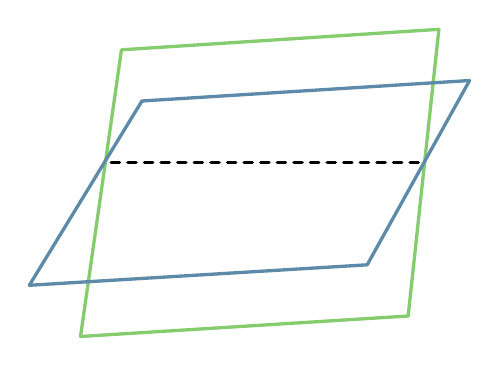
\begin{tikzpicture}[line cap=round, line join=round, >=Triangle,scale=1.3]
    	\coordinate (A1) at (0.0,0.0);
    	\coordinate (B1) at (0.4,2.8);
    	\coordinate (C1) at (3.5,3.0);
    	\coordinate (D1) at (3.2,0.2);
    	
    	\coordinate (A2) at (-0.5,0.5);
    	\coordinate (B2) at (0.6,2.3);
    	\coordinate (C2) at (3.8,2.5);
    	\coordinate (D2) at (2.8,0.7);
    	
		\draw [-,nicegreen,line width=1.2pt] (A1)--(B1);
		\draw [-,nicegreen,line width=1.2pt] (B1)--(C1);
		\draw [-,nicegreen,line width=1.2pt] (C1)--(D1);
		\draw [-,nicegreen,line width=1.2pt] (D1)--(A1);
    	
		\draw [-,airforceblue,line width=1.2pt] (A2)--(B2);
		\draw [-,airforceblue,line width=1.2pt] (B2)--(C2);
		\draw [-,airforceblue,line width=1.2pt] (C2)--(D2);
		\draw [-,airforceblue,line width=1.2pt] (D2)--(A2);

		\draw [dashed,black,line width=1.2pt] (0.3,1.7)--(3.3,1.7);
    \end{tikzpicture}
    \caption*{These 2 planes intersect at a line, the infinite points of which are the solutions to the two equations.}
\end{subfigure}
\hfill
\begin{subfigure}{.45\textwidth}
    \centering
    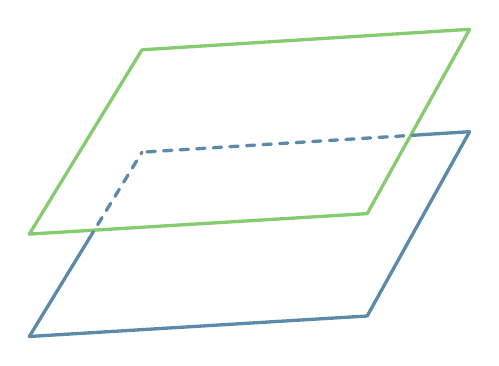
\begin{tikzpicture}[line cap=round, line join=round, >=Triangle,scale=1.3]
    	\coordinate (A1) at (-0.5,1.5);
    	\coordinate (B1) at (0.6,3.3);
    	\coordinate (C1) at (3.8,3.5);
    	\coordinate (D1) at (2.8,1.7);
    	
    	\coordinate (A2) at (-0.5,0.5);
    	\coordinate (B2) at (0.6,2.3);
    	\coordinate (C2) at (3.8,2.5);
    	\coordinate (D2) at (2.8,0.7);
    	
		\draw [-,nicegreen,line width=1.2pt] (A1)--(B1);
		\draw [-,nicegreen,line width=1.2pt] (B1)--(C1);
		\draw [-,nicegreen,line width=1.2pt] (C1)--(D1);
		\draw [-,nicegreen,line width=1.2pt] (D1)--(A1);
    	
		\draw [-,airforceblue,line width=1.2pt] (A2)--($0.47*(A2)+0.53*(B2)$);
		\draw [dashed,airforceblue,line width=1.2pt] ($0.47*(A2)+0.53*(B2)$)--(B2);
		\draw [-,airforceblue,line width=1.2pt] (C2)--($0.85*(C2)+0.15*(B2)$);
		\draw [dashed,airforceblue,line width=1.2pt] ($0.85*(C2)+0.15*(B2)$)--(B2);
		\draw [-,airforceblue,line width=1.2pt] (C2)--(D2);
		\draw [-,airforceblue,line width=1.2pt] (D2)--(A2);
    \end{tikzpicture}
    \caption*{These 2 planes are simply offset and never intersect. Hence there are no solutions.}
\end{subfigure}
\end{figure}


\example{Undetermined system with infinite solutions}{
Consider the following \textbf{underdetermined system}
\begin{align*}
(S)
\left\{
\begin{matrix}
    x &  +3y &   -z &  +4t &=&   27 \\
  -4x & -11y &  +6z & -14t &=& -105 \\
  -2x & -10y &  -7z & -14t &=&  -55
\end{matrix}
\right.
\end{align*}
After some lines of the usual Gaussian method, we arrive at 
\begin{align*}
\left(
	\begin{matrix}
	   1 &   3 &  -1 &   4 \\
	   0 &   1 &   2 &   2 \\
	   0 &   0 &  -1 &   2
	\end{matrix}
  \left|
	\begin{matrix}
	    27 \\
	     3 \\
	    11 \\
	\end{matrix}
  \right.
\right)
\end{align*}
We already solved this system. The infinite solutions are:
\begin{align*}
\begin{pmatrix}
   x \\
   y \\
   z \\
   t
\end{pmatrix}
=
\begin{pmatrix}
   16t - 59 \\
   -6t + 25\\
    2t - 11\\
     t
\end{pmatrix}
=
\begin{pmatrix}
   16 \\
    -6 \\
   2\\
   1
\end{pmatrix}
t
+
\begin{pmatrix}
   -59 \\
    25 \\
   -11 \\
     0
\end{pmatrix}
\end{align*}
}



\section{Cramer systems and Cramer's rule}



\definition{Cramer system}{
Suppose we have the following linear system of equations (with unknowns equal to equations)
\begin{align*}
\begin{cases}
a_{11} x_1  + a_{12} x_2 + \cdots + a_{1n} x_n = y_1 \\
a_{21} x_1  + a_{22} x_2 + \cdots + a_{2n} x_n = y_2 \\
\vdots \\
a_{n1} x_1  + a_{n2} x_2 + \cdots + a_{nn} x_n = y_n
\end{cases}
\qquad (S)
\end{align*}
with the associated matrix form
\begin{align*}
\underbrace{
\begin{pmatrix}
a_{11} & a_{12} & \cdots & a_{1n} \\
a_{21} & a_{22} & \cdots & a_{2n} \\
\vdots & \vdots & \ddots & \vdots \\
a_{n1} & a_{n2} & \cdots & a_{nn}
\end{pmatrix}}_A
%%
%%
\underbrace{
\begin{pmatrix}
x_{1} \\
x_{2} \\
\vdots \\
x_{n}
\end{pmatrix}}_X
%%
=
\underbrace{
\begin{pmatrix}
y_{1} \\
y_{2} \\
\vdots \\
y_{n}
\end{pmatrix}}_Y
\end{align*}
We say that $(S)$ is a Cramer system if $\det(A) \neq 0$.
}

\theorem{Cramer's rule}{
The unique solution to a Cramer system, $X$, has coefficients given by Cramer's rule:
\begin{align*}
x_i = \dfrac{1}{\det(A)}
\underbrace{
\left|
\begin{matrix}
a_{11} & \cdots & a_{1,i-1} & y_1 & a_{1,i+1} & \cdots & a_{1n} \\
a_{21} & \cdots & a_{2,i-1} & y_2 & a_{2,i+1} & \cdots & a_{2n} \\
\vdots & \cdots & \vdots    & \vdots & \vdots & \ddots & \vdots \\
a_{n1} & \cdots & a_{n,i-1} & y_n & a_{n,i+1} & \cdots & a_{nn}
\end{matrix}
\right|
}_{\text{Replace the ith column with Y}}
\quad \text{for every $i$}
\end{align*}

Note that this means we must take $n$ different determinants of this style, one for each unknown in the $X$ column.
}


\example{Cramer's rule}{

Let's use Cramer’s rule to find the solutions to the system $(S)$ with the following associated coefficient matrices and constant columns
\begin{align*}
A =& 
\begin{pmatrix}
3 & 1 & 5 \\
2 & 1 & 2 \\
0 & 3 & 7 
\end{pmatrix}
\quad
Y = 
\begin{pmatrix}
2 \\ 1 \\ 3
\end{pmatrix}
\qquad (S)
\end{align*}
We first need the determinant of the matrix
\begin{align*}
\det(A) = 3\left| \begin{matrix} 1 & 2 \\ 3 & 7 \end{matrix} \right|
- 2\left| \begin{matrix} 1 & 5 \\ 3 & 7 \end{matrix} \right|
= 3(7-6) - 2(7-15) = 19
\end{align*}
Then we apply Cramer's rule to find each of the three solution coefficients:
\begin{align*}
x_1 &= \frac{1}{\det(A)}
  \left|\begin{array}{>{\columncolor{airforceblue!20}}ccc}
	2 & 1 & 5 \\
	1 & 1 & 2 \\
	3 & 3 & 7 
  \end{array}\right|
  = \frac{1}{19}\left(
  	  2\left|\begin{matrix} 1 & 2 \\ 3 & 7 \end{matrix}\right| 
  	 -5\left|\begin{matrix} 1 & 2 \\ 3 & 7 \end{matrix}\right|
  	 +5\left|\begin{matrix} 1 & 1 \\ 3 & 3 \end{matrix}\right|
  	\right)
  = \frac{1}{19}
%%
\\
%%
x_2 &= \frac{1}{\det(A)}
  \left|\begin{array}{c>{\columncolor{airforceblue!20}}cc}
	3 & 2 & 5 \\
	2 & 1 & 2 \\
	0 & 3 & 7 
  \end{array}\right|
  = \frac{1}{19}\left(
  	  3\left|\begin{matrix} 1 & 2 \\ 3 & 7 \end{matrix}\right| 
  	 -2\left|\begin{matrix} 2 & 2 \\ 0 & 7 \end{matrix}\right|
  	 +5\left|\begin{matrix} 2 & 1 \\ 0 & 3 \end{matrix}\right|
  	\right)
  = \frac{5}{19}\vspace{-0.5cm}
%%
\\
%%
x_3 &= \frac{1}{\det(A)}
  \left|\begin{array}{cc>{\columncolor{airforceblue!20}}c}
	3 & 1 & 2 \\
	2 & 1 & 1 \\
	0 & 3 & 3 
  \end{array}\right|
  = \frac{1}{19}\left(
  	  3\left|\begin{matrix} 1 & 1 \\ 3 & 3 \end{matrix}\right| 
  	 -1\left|\begin{matrix} 2 & 1 \\ 0 & 3 \end{matrix}\right|
  	 +2\left|\begin{matrix} 2 & 1 \\ 0 & 3 \end{matrix}\right|
  	\right)
  = \frac{6}{19}
\end{align*}
So the unique solution to $(S)$ is $(x_1,x_2,x_3)=\dfrac{1}{19}(1,5,6)$
}
%%%%%%%%%%%%%%%%%%%%%%%%%%%%%%%%%%%%%%%%%%%%%%%%%%%%%%%%%%%%%%%%%%%%%%%%

%\end{document}

\pagenumbering{roman}

\ifnum \version = 1
	\input{TitlePage_I1.tex}
	
	%\null\newpage 
	
	% List of Definitions and Theorems
	\renewcommand{\listtheoremname}{List of Definitions}
	\listoftheorems[ignoreall,show=definitionnew]
	\clearpage

	\clearpage
	\pagenumbering{arabic}
	\chapter{Euclidean Vectors} \label{ch:euclid}


\definition{Euclidean vector or tuple}{
A Euclidean vector is a list of $n$ real numbers, also called an $n$-tuple. We write this list in parentheses, for example $(1,3,-2, \dots, 0)$, and we say that this object belongs to $\mathbb{R}^n$. An arbitrary tuple can be written $\mathbf{v}=(v_1,v_2,\cdots,v_n)$ where the \textit{components} $v_i \in \mathbb{R}$ for any index $i$.
}


\definition{Tuple addition}{
Euclidean vectors are added to each other component by component. In symbols
\begin{align*}
(a_1, a_2, \dots, a_n) + (b_1, b_2, \dots, b_n) = (a_1+b_1, a_2+b_2, \dots, a_n + b_n).
\end{align*}
\textit{Note}: this means you can only add two tuples together \textit{of the same size}. It makes no sense to add a 3-tuple to a 5-tuple.
}


\definition{Scalar multiplication}{
Let $c\in\mathbb{R}$, called a scalar quantity, and $\mathbf{v} \in \mathbb{R}^n$ with components $v_i$. Then the \textit{scalar multiplication} $c\mathbf{v}$ gives a vector $\mathbf{w}$ with components $w_i = c v_i$ for every index $i$. In tuple form
\begin{align*}
c(v_1,v_2,\dots,v_n) = (cv_1,cv_2,\dots,cv_n).
\end{align*}
}


\definition{Canonical Euclidean unit vectors}{
The canonical Euclidean vectors in $\mathbb{R}^n$ are the $n$ vectors of the form
\begin{gather*}
\mathbf{e}_1 = (1,0,\dots,0) \\
\mathbf{e}_2 = (0,1,\dots,0) \\
\vdots \\
\mathbf{e}_n = (0,0,\dots,1).
\end{gather*}
More compactly
\begin{align*}
\mathbf{e}_k = (\alpha_1, \alpha_2, \dots, \alpha_n) \quad \text{where} \quad
\alpha_j=
\begin{cases}
1 & \text{for } j= k, \\
0 & \text{for } j\neq k.
\end{cases}
\end{align*}
}


\definition{Dot product}{
For two $n$-tuples $\mathbf{a}$ and $\mathbf{b}$, their \textit{dot product}, also called \textit{scalar} product and \textit{Euclidean inner} product, is the real number given by the addition of component by component multiplication
\begin{align*}
\mathbf{a}\cdot\mathbf{b} = a_1 b_1 + a_2 b_2 + \cdots + a_n b_n = \sum_{i=1}^n a_i b_i.
\end{align*}
}

\definition{Euclidean Norm}{
The norm of an $n$-tuple $\mathbf{v}$, denoted $\lVert \mathbf{v} \rVert$, is given by
\begin{align*}
\lVert \mathbf{v} \rVert = \sqrt{\mathbf{v}\cdot\mathbf{v}} = \sqrt{v_1^2 + v_2^2 + \cdots + v_2^2}.
\end{align*}
}

\definition{Orthogonal Euclidean vectors}{
Two vectors in $\mathbb{R}^n$ are orthogonal if and only if their dot product equals zero.
}

\definition{Displacement vector}{
Given two Euclidean vectors $\mathbf{a}$ and $\mathbf{b}$, the displacement vector pointing from $\mathbf{a}$ to $\mathbf{b}$ is given by $\mathbf{r}=\mathbf{b}-\mathbf{a}$ as pictured below. Of course we can also create the displacement vector in the other direction, from $\mathbf{b}$ to $\mathbf{a}$, given by $\mathbf{a}-\mathbf{b}$.
}


\definition{Vector form of a straight line}{
The set of vectors in $\mathbb{R}^n$ of the form $\mathbf{v} = \mathbf{a} + t \mathbf{r}$ for a parameter $t\in\mathbb{R}$ represents a straight line through the space $\mathbb{R}^n$. That is,
\begin{align*}
\{(x,y) \, | \, \forall x\in\mathbb{R} \, \text{and} \, y=mx+b  \} = \{ \mathbf{a} + t \mathbf{r} \, | \, \forall t\in\mathbb{R} \}
\end{align*}
where $\mathbf{a}$ is an arbitrary pair $(x,mx+b)$ and $\mathbf{r}$ is a displacement vector between any two distinct pairs $(x_1,mx_1+b)$ and $(x_2,mx_2+b)$.
}


	\chapter{Matrix Algebra} \label{ch:matrixalgebra}


\definition{Matrix}{
A matrix is a collection of numbers from a field $\mathbb{F}$ (e.g. rational numbers) usually represented by a rectangular array. For example, an $m \times n$ (said m by n) matrix $A$ with coefficients $a_{ij}\in\mathbb{F}$  would be represented by an array with $m$ rows and $n$ columns:
\begin{align*}
A = 
\begin{pmatrix}
a_{11} & a_{12} & a_{13} & \cdots & a_{1j} & \cdots & a_{1m} \\
a_{21} & a_{22} & a_{23} & \cdots & a_{2j} & \cdots & a_{2m} \\
a_{31} & a_{32} & a_{33} & \cdots & a_{3j} & \cdots & a_{3m} \\
\vdots & \vdots & \vdots & \ddots & \vdots & \ddots & \vdots \\
a_{i1} & a_{12} & a_{13} & \cdots & a_{ij} & \cdots & a_{im} \\
\vdots & \vdots & \vdots & \ddots & \vdots & \ddots & \vdots \\
a_{n1} & a_{n2} & a_{n3} & \cdots & a_{nj} & \cdots & a_{nm}
\end{pmatrix}
=
\left( a_{ij} \right)_{\substack{ 1 \leq i \leq m \\ 1 \leq j \leq n }}.
\end{align*}
Sometimes it is convenient to refer to the coefficients in the array like so: $a_{ij} = \left(A\right)_{ij}$.
}

\definition{Set of all $m \times n$ matrices}{
We write the set of all $m \times n$ matrices with coefficients in $\mathbb{F}$ as
\begin{align*}
\mathcal{M}_{m,n}(\mathbb{F})
\end{align*}
}

\definition{Matrix columns and rows}{
For a matrix $A\in\mathcal{M}_{m,n}(\mathbb{F})$ we denote its j$^{th}$ column and i$^{th}$ row
\begin{align*}
A^{(j)} =
\begin{pmatrix}
 a_{1j} \\
 a_{2j} \\
 a_{3j} \\
 \vdots \\
 a_{ij} \\
 \vdots \\
 a_{mj}
\end{pmatrix},
\qquad
A_{(i)} =
\begin{pmatrix}
a_{i1} & a_{12} & a_{13} & \cdots & a_{ij} & \cdots & a_{in}
\end{pmatrix}
\end{align*}
}

\definition{Transpose of a matrix}{
The transpose of an $m \times n$ matrix, $A$, is an $n \times m$ matrix, denoted $A^T$, with rows equal to the columns of $A$. That is, $\left(A^T\right)_{ij} = \left(A\right)_{ji}$ for all combinations of $i$ and $j$. 
}



\definition{Diagonal matrix}{
A square matrix $A$ is said to be diagonal if all its non-diagonal elements are zero, e.g. $(A)_{ij}=0$ whenever $i \neq j$.
}

\definition{Symmetric matrix}{
A matrix $A$ is symmetric if it is equal to its transpose, $A = A^T$.
}



\definition{Matrix addition}{
Matrix addition is done coefficient by coefficient, that is, for two matrices $A$ and $B$ we define the i,j$^{th}$ coefficient of the addition as the addition of the i,j$^{th}$ coefficients of each matrix: 
\begin{align*}
\left(A+B\right)_{ij} = \left(A\right)_{ij}+\left(B\right)_{ij}.
\end{align*}
}



\definition{Scalar multiplication}{
Given a number $k\in\mathbb{R}$ (called a scalar) and a matrix $A \in \mathcal{M}_{m,n}$, we define matrix scalar multiplication, $kA$, to be a matrix $B \in \mathcal{M}_{m,n}$ with coefficients given by:
\begin{align*}
b_{ij} = ka_{ij},
\end{align*}
that is, we multiply \textit{every coefficient} by the scalar.
} 


\definition{Zero matrix}{
The zero matrix of any shape is a matrix $M_0 \in\mathcal{M}_{m,n}$ consisting entirely of zeros as coefficients.
} 


\definition{Additive inverse}{
Given a matrix $A\in\mathcal{M}_{ij}$, its additive inverse is the same matrix multiplied by the scalar $-1$. We denote the additive inverse of $A$ as $-A$.
} 


\definition{Multiplication of a matrix by a column}{
Consider a matrix $A \in \mathcal{M}_{m,n}$ and a column $X \in \mathcal{M}_{n,1}$. We define the product $AX$ to result in the column $Y\in\mathcal{M}_{m,1}$ with coefficients
\begin{align*}
(Y)_i = a_{i1}x_1 + a_{i2}x_2 + \cdots + a_{im}x_m = \sum_{k=1}^m a_{ik} x_k 
\end{align*}
Visually
\begin{align*}
\begin{pmatrix}
y_{1} \\
y_{2} \\
\vdots \\
y_{n} 
\end{pmatrix}
%%%
%%%
%%%
&=
%%%
\begin{pmatrix}
a_{11} & a_{12} & \cdots & a_{1m} \\
a_{21} & a_{22} & \cdots & a_{2m} \\
\vdots & \vdots & \ddots & \vdots \\
a_{n1} & a_{n2} & \cdots & a_{nm}
\end{pmatrix}
\begin{pmatrix}
x_{1} \\
x_{2} \\
\vdots \\
x_{m} 
\end{pmatrix}
%%%
%%%
%%%
=
%%%
x_{1}
\begin{pmatrix}
a_{11} \\
a_{21} \\
\vdots \\
a_{n1} 
\end{pmatrix}
+
x_{2}
\begin{pmatrix}
a_{12} \\
a_{22} \\
\vdots \\
a_{n2} 
\end{pmatrix}
+ \cdots +
x_m
\begin{pmatrix}
a_{1m} \\
a_{2m} \\
\vdots \\
a_{nm} 
\end{pmatrix}
\\ \\
%%%
%%%
%%%
&\implies Y = x_{1}A^{(1)} + x_{2}A^{(2)} + \cdots + x_{m}A^{(m)}
\end{align*}
}

\definition{Rotation matrix - arbtirary angle anti-clockwise}{
By using a column $X\in\mathcal{M}_{2,1}$ to represent a Euclidean vector, the following matrix allows the operation of rotataion, anti-clockwise, of $X$ by an angle $\theta$:
\begin{align*}
R_\theta =
\begin{pmatrix} 
\cos\theta & -\sin\theta \\ 
\sin\theta &  \cos\theta  
\end{pmatrix}
\end{align*}
where the rotated vector is represented by a column $X'\in\mathcal{M}_{2,1}$ obtained by matrix multiplication $X' = R_\theta X$.
}


\definition{Multiplication of two matrices}{
Consider two matrices $A \in \mathcal{M}_{n,m}$ and $B \in \mathcal{M}_{m,q}$. We define the product $AB$ to be the matrix $C\in\mathcal{M}_{n,q}$ with coefficients
\begin{gather*}
c_{ij} = a_{i1}b_{1j} + a_{i2}b_{2j} + \cdots + a_{im}b_{mj} = \sum_{k=1}^m a_{ik} b_{kj} \\
%%%
%%%
%%%
\implies
\begin{pmatrix}
a_{11} & a_{12} & \cdots & a_{1m} \\
a_{21} & a_{22} & \cdots & a_{2m} \\
\vdots & \vdots & \ddots & \vdots \\
a_{n1} & a_{n2} & \cdots & a_{nm}
\end{pmatrix}
\begin{pmatrix}
b_{11} & b_{12} & \cdots & b_{1q} \\
b_{21} & b_{22} & \cdots & b_{2q} \\
\vdots & \vdots & \ddots & \vdots \\
b_{m1} & b_{m2} & \cdots & b_{mq}
\end{pmatrix} \\
%%%
%%%
%%%
=
\left(
b_{11}
\underbrace{
\begin{pmatrix}
a_{11} \\
a_{21} \\
\vdots \\
a_{n1} 
\end{pmatrix}
+ \cdots +
b_{m1}
\begin{pmatrix}
a_{1m} \\
a_{2m} \\
\vdots \\
a_{nm} 
\end{pmatrix}
}_{\text{\large first column}}
%%
\quad \cdots \quad 
%%
b_{1q}
\underbrace{
\begin{pmatrix}
a_{11} \\
a_{21} \\
\vdots \\
a_{n1} 
\end{pmatrix}
+ \cdots +
b_{mq}
\begin{pmatrix}
a_{1m} \\
a_{2m} \\
\vdots \\
a_{nm} 
\end{pmatrix}
}_{\text{\large n$^{th}$ column}}
\right)
\end{gather*}
Additionally, for the product
\begin{align*}
\underbrace{A}_{(\colorbox{Mahogany!20}{n},\colorbox{airforceblue!20}{m})} \underbrace{B}_{(\colorbox{airforceblue!20}{m},\colorbox{Mahogany!20}{q})}
\end{align*}
we will call the indices for the columns of $A$ and rows of $B$ the \textit{inner indices} (blue), whereas the indices for the rows of $A$ and columns of $B$ will be called the \textit{outer indices} (red).
}

\definition{Identity matrix}{
The $n$-dimensional identity matrix $I$ is a square matrix of size $n\times n$ with 1s along the diagonal and 0s elsewhere, that is, 
\begin{align*}
(I)_{ij}
=
\begin{cases}
1 & \text{whenever } \, i=j, \\
0 & \text{whenever } \, i \neq j.
\end{cases}
\end{align*}
}

\definition{Invertible matrix}{
A matrix $A$ is invertible if and only if there exists a matrix $B$ such that
\begin{align*}
A B = BA = I
\end{align*}
This matrix $B$ is called the inverse of $A$ and is denoted $A^{-1}$. As we have commutative matrices, $AB=BA$, recall that this can only happen if $A$ is square. So, only square matrices can have inverses.
}

\definition{Determinant of a 1 by 1 matrix}{
The determinant of any 1 by 1 matrix is given by its only coefficient:

\begin{align*}
\det \left( \begin{pmatrix} a \end{pmatrix}\right)  = a
\end{align*}
}


\definition{Submatrix}{
From a matrix $A$ we generate the \textit{submatrix} $A_{ij}$ by deleting the $ith$ row and $jth$ column:
\begin{align*}
\text{For} \, A =
\begin{pmatrix}
a_{1,1}   & \cdots & a_{1,j-1}   & a_{1,j}   & a_{1,j+1}   & \cdots & a_{1,n}   \\
\vdots    & \cdots & \vdots      & \vdots    & \vdots      & \cdots & \vdots    \\
a_{i-1,1} & \cdots & a_{i-1,j-1} & a_{i-1,j} & a_{i-1,j+1} & \cdots & a_{i-1,n} \\
a_{i,1}   & \cdots & a_{i,j-1}   & a_{i,j}   & a_{i,j+1}   & \cdots & a_{i,n}   \\
a_{i+1,1} & \cdots & a_{i+1,j-1} & a_{i+1,j} & a_{i+1,j+1} & \cdots & a_{i+1,n} \\
\vdots    & \cdots & \vdots      & \vdots    & \vdots      & \cdots & \vdots    \\
a_{m,1}   & \cdots & a_{m,j-1}   & a_{m,j}   & a_{m,j+1}   & \cdots & a_{m,n} 
\end{pmatrix} \\
\text{The submatrix} \, A_{ij} =
\begin{pmatrix}
a_{1,1}   & \cdots & a_{1,j-1}   & a_{1,j+1}   & \cdots & a_{1,n}   \\
\vdots    & \cdots & \vdots      & \vdots      & \cdots & \vdots    \\
a_{i-1,1} & \cdots & a_{i-1,j-1} & a_{i-1,j+1} & \cdots & a_{i-1,n} \\
a_{i+1,1} & \cdots & a_{i+1,j-1} & a_{i+1,j+1} & \cdots & a_{i+1,n} \\
\vdots    & \cdots & \vdots      & \vdots      & \cdots & \vdots    \\
a_{m,1}   & \cdots & a_{m,j-1}   & a_{m,j+1}   & \cdots & a_{m,n} 
\end{pmatrix}
\end{align*}
\textit{Note}: we generally have to specify in words that we create a submatrix. The notation $A_{ij}$ is a little ambiguous without being explicit. 
}


\definition{Determinant of an $n \times n$ matrix}{
For any square matrix $A\in\mathcal{M}_{n,n}$, its determinant is given by
\begin{align*}
\det(A) = \sum_{i=1}^n (-1)^{i+j} a_{ij} \det(A_{ij})
\end{align*}
where the $a_{ij}$ are coefficients of $A$, $A_{ij}$ is the $i,j^{th}$ submatrix of $A$ and for any $1\leq j \leq n$. We can also sum over the $j$ index for any $1\leq i \leq n$
\begin{align*}
\det(A) = \sum_{j=1}^n (-1)^{i+j} a_{ij} \det(A_{ij})
\end{align*}
and we will show that the answer is the same.
}

\definition{Cramer system}{
Suppose we have the following linear system of equations (with unknowns equal to equations)
\begin{align*}
\begin{cases}
a_{11} x_1  + a_{12} x_2 + \cdots + a_{1n} x_n = y_1 \\
a_{21} x_1  + a_{22} x_2 + \cdots + a_{2n} x_n = y_2 \\
\vdots \\
a_{n1} x_1  + a_{n2} x_2 + \cdots + a_{nn} x_n = y_n
\end{cases}
\qquad (S)
\end{align*}
with the associated matrix form
\begin{align*}
\underbrace{
\begin{pmatrix}
a_{11} & a_{12} & \cdots & a_{1n} \\
a_{21} & a_{22} & \cdots & a_{2n} \\
\vdots & \vdots & \ddots & \vdots \\
a_{n1} & a_{n2} & \cdots & a_{nn}
\end{pmatrix}}_A
%%
%%
\underbrace{
\begin{pmatrix}
x_{1} \\
x_{2} \\
\vdots \\
x_{n}
\end{pmatrix}}_X
%%
=
\underbrace{
\begin{pmatrix}
y_{1} \\
y_{2} \\
\vdots \\
y_{n}
\end{pmatrix}}_Y
\end{align*}
We say that $(S)$ is a Cramer system if $\det(A) \neq 0$.
}

\definition{Cofactor matrix}{
From a matrix $A$ we generate its cofactor matrix $C_A$ which has entries given by determinants of submatrices of $A$ with the same plus/minus pattern as in a determinant calculation. That is, the entries of $C_A$ are $c_{ij}=(-1)^{i+j} \det(A_{ij})$:
\begin{align*}
C_A =
\begin{pmatrix}
 |A_{11}| & -|A_{12}| &  |A_{13}| & \cdots   \\
-|A_{21}| &  |A_{22}| & -|A_{23}| & \cdots   \\
 |A_{31}| & -|A_{32}| &  |A_{33}| & \cdots   \\
 \vdots   &  \vdots   &  \vdots   & \ddots
\end{pmatrix}
\end{align*}
}


	\chapter{Linear Systems} \label{ch:linearsystems}


\definition{Linear system of equations}{
A system of $m$ linear equations with $n$ unknowns, denoted $(S)$, has the general form
\begin{align*}
\begin{cases}
a_{11} x_1  + a_{12} x_2 + \cdots + a_{1n} x_n = y_1 \\
a_{21} x_1  + a_{22} x_2 + \cdots + a_{2n} x_n = y_2 \\
\vdots \\
a_{m1} x_1  + a_{m2} x_2 + \cdots + a_{mn} x_n = y_m
\end{cases}
\qquad (S)
\end{align*}
where the $x_j$ are the unknowns we want to find, $a_{ij}$ are the \textit{coefficients} and  the $y_i$ are the \textit{constant terms}.
}

\definition{Homogeneous linear system}{
For any system of linear equations, $(S)$, given by $AX=Y$, we associate the \textbf{homogeneous system}, denoted $(H)$:
\begin{align*}
 AX = 0_m
\end{align*} 
for the column
\begin{align*}
0_m = \begin{pmatrix} 0 \\ 0 \\ \vdots \\ 0 \end{pmatrix} \in \mathcal{M}_{m,1}
\end{align*}
We will denote the solution set of $(H)$ by $\mathcal{H}$.

\noindent \textit{Note}: the homogeneous system always admits \textit{at least one} solution, the trivial solution $X=0_n$.
}



\definition{Equivalent systems}{
Two systems of linear equations are \textbf{equivalent} if they share the same set of solutions.
}

\definition{Elementary operations}{

There are \textbf{elementary operations} that we can do to systems of equations that give new systems that remain equivalent to the old.

\centering

\underline{Exchanging two equations} \vspace{-0.4cm}
\begin{align*}
(S_1)
\begin{cases}
    I_1 +   I_2 -   I_3 =  0 \\
 13 I_1 - 6 I_2         = 20 
\end{cases}
\quad\equiv\quad
(S_2)
\begin{cases}
 13 I_1 - 6 I_2         = 20 \\
    I_1 +   I_2 -   I_3 =  0 
\end{cases}
\end{align*}
\underline{Multiplying one equation by a non-zero constant} \vspace{-0.4cm}
\begin{align*}
(S_1)
\begin{cases}
    I_1 +   I_2 -   I_3 =  0 \\
 13 I_1 - 6 I_2         = 20 
\end{cases}
\quad\equiv\quad
(S_2)
\begin{cases}
    I_1 +   I_2 -   I_3 =  0 \\
 I_1 - (6/13) I_2         = (20/13) 
\end{cases}
\end{align*}
\underline{Adding a multiple of one equation to another equation} \vspace{-0.4cm}
\begin{align*}
(S_1)
\begin{cases}
    I_1 +   I_2 -   I_3 =  0 \\
 13 I_1 - 6 I_2         = 20 
\end{cases}
\quad\equiv\quad
(S_2)
\begin{cases}
    I_1 +   I_2 -   I_3 =  0 \\
 15 I_1 - 4 I_2 - 2 I_3 = 20 
\end{cases}
\end{align*}
}


\definition{Overdetermined system}{
An overdetermined system has more equations than unknowns. We say “there are too many equations”. Such a system allows solutions only if certain conditions are met. 
}


\definition{Underdetermined system}{

An \textbf{underdetermined system} has less equations than unknowns. We say ``there are not enough equations''. Such a system has either no solutions, or infinitely many. 
}


\definition{Cramer system}{
Suppose we have the following linear system of equations (with unknowns equal to equations)
\begin{align*}
\begin{cases}
a_{11} x_1  + a_{12} x_2 + \cdots + a_{1n} x_n = y_1 \\
a_{21} x_1  + a_{22} x_2 + \cdots + a_{2n} x_n = y_2 \\
\vdots \\
a_{n1} x_1  + a_{n2} x_2 + \cdots + a_{nn} x_n = y_n
\end{cases}
\qquad (S)
\end{align*}
with the associated matrix form
\begin{align*}
\underbrace{
\begin{pmatrix}
a_{11} & a_{12} & \cdots & a_{1n} \\
a_{21} & a_{22} & \cdots & a_{2n} \\
\vdots & \vdots & \ddots & \vdots \\
a_{n1} & a_{n2} & \cdots & a_{nn}
\end{pmatrix}}_A
%%
%%
\underbrace{
\begin{pmatrix}
x_{1} \\
x_{2} \\
\vdots \\
x_{n}
\end{pmatrix}}_X
%%
=
\underbrace{
\begin{pmatrix}
y_{1} \\
y_{2} \\
\vdots \\
y_{n}
\end{pmatrix}}_Y
\end{align*}
We say that $(S)$ is a Cramer system if $\det(A) \neq 0$.
}

	\chapter{Vector Spaces} \label{ch:vectorspaces}


\definition{Vector space}{
A \textit{vector space over a field} $\mathbb{F}$ is a set, call it $V$, with elements called vectors supplied with definitions of two operations, \textit{vector addition} (VA) and \textit{scalar multiplication} (SM), that satisfy the following \textit{vector space axioms}:
\begin{align*}
& \forall \, \mathbf{u},\mathbf{v},\mathbf{w} \in V \quad \text{and} \quad \forall \, k,l \in \mathbb{F} \\
\text{(VA1)} & \quad \mathbf{u} + \mathbf{v} \in V  & (\text{closure under vector addition})\\
%
\text{(VA2)} & \quad (\mathbf{u} + \mathbf{v}) + \mathbf{w}  =\mathbf{u} + (\mathbf{v} + \mathbf{w} ) & (\text{associativity of vector addition})\\
%
\text{(VA3)} & \quad \exists \, \mathbf{0} \in V, \, \text{such that} \, \mathbf{u} + \mathbf{0} = \mathbf{0} + \mathbf{u} = \mathbf{u} & (\text{additive identity})\\
%
\text{(VA4)} & \quad \exists \, -\mathbf{u} \in V \, \text{such that} \, \mathbf{u} + (-\mathbf{u}) = \mathbf{0} & (\text{additive inverse})\\
%
\text{(VA5)} & \quad \mathbf{u} + \mathbf{v} = \mathbf{v} + \mathbf{u} & (\text{commutativity of vector addition})\\
%
\text{(SM1)} & \quad k\mathbf{u} \in V & (\text{closure under scalar multiplication})\\
%
\text{(SM2)} & \quad k(\mathbf{u}+\mathbf{v})=k\mathbf{u}+k\mathbf{v} & (\text{distributivity over vector addition})\\
%
\text{(SM3)} & \quad (k+l)\mathbf{u}=k\mathbf{u}+l\mathbf{u} & (\text{distributivity over field addition})\\
%
\text{(SM4)} & \quad k(l\mathbf{u})=(kl)\mathbf{u} & (\text{compatibility of scalar and field multiplication})\\
%
\text{(SM5)} & \quad 1\mathbf{u}=\mathbf{u} & (\text{multiplicative identity})
\end{align*}
}

\definition{Linear Combination}{
Let \{$\mathbf{v}_1$, \dots, $\mathbf{v}_n$\} be a set of vectors in a vector space $V$. A linear combination of these vectors is a new vector, $\mathbf{w}\in V$, of the form
\begin{align*}
\mathbf{w} = \alpha_1 \mathbf{v}_1 + \cdots + \alpha_n \mathbf{v}_n
\end{align*}
where the $\alpha_k$ are real numbers.
}


\definition{Vector subspace}{
Suppose that $V$ is a vector space and $W$ is a subset of $V$. We call $W$ a \textit{vector subspace} if it satisfies the vector space axioms for the same definition of vector addition and scalar multiplication defined for $V$.
}


\definition{Span}{
Let $\mathcal{B} = \{\mathbf{v}_1, \dots, \mathbf{v}_n\}$ be a set of vectors from a vector space $V$. The span of these vectors is the set of all linear combinations of those vectors:
\begin{align*}
\text{SPAN}(\mathcal{B})  = \text{SPAN} (\mathbf{v}_1, \dots, \mathbf{v}_n) = \left\{ \alpha_1 \mathbf{v}_1 + \cdots + \alpha_n \mathbf{v}_n \, | \, \forall \alpha_1, \dots, \alpha_n \in \mathbb{R}^n \right\}.
\end{align*}
This set forms a vector subspace of $V$. It is obviously non-empty because it at least contains the vectors of $\mathcal{B}$. It is also automatically closed under vector addition and scalar multiplication because those are exactly the operations we used to create all the vectors in the span! Therefore $\text{SPAN}(\mathcal{B})$ is a vector subspace of $V$.
}


\definition{Cartesian form of Euclidean vector sub spaces}{
Euclidean vector sub spaces can always be written as a set with some defining equations:
\begin{align*}
\left\{ (x_1,\dots,x_n) \in \mathbb{R}^n \, | \, \text{equations relating the } x_k \right\}.
\end{align*}
For example, the general form of planar vector subspaces of $\mathbb{R}^3$ is
\begin{align*}
V_P = \left\{ (x,y,z)\in \mathbb{R}^3 \, | \, ax + by + cz = 0\right\}
\end{align*}
where $a$, $b$ and $c$ are some given constants. This set is read aloud as ``all the triples $(x,y,z)$ such that $ax + by + cz = 0$''.
}


\definition{Sum of subspaces (sum space)}{
Suppose we have a vector space $V$ with vector subspaces $F$ and $G$. We define the \textbf{sum of subspaces} (or sum space) as a new set denoted
\begin{align*}
F + G = \left\{ \textbf{f} + \textbf{g} \, | \, \textbf{f}\in F, \, \textbf{g}\in G\right\}
\end{align*}

\noindent \textit{Note}: The sum space is a \textit{subset} of the parent vector space: $F+G \subset V$.
}


\definition{Direct sum}{
Let $F$ and $G$ be two vector subspaces of a vector space $V$ and let $E=F+G$ be the sum space. We say $E$ is a \textbf{direct sum} of $F$ and $G$ if each element of $E$ has a \textbf{unique} decomposition as a sum of vectors in $F$ and vectors in $G$. That is, for every $\textbf{v}\in E$, there exists unique vectors $\textbf{f}\in F$ and $\textbf{g}\in G$ such that $\textbf{v} = \textbf{f} + \textbf{g}$. We denote this direct sum with a new symbol
\begin{align*}
E = F \oplus G
\end{align*}
}


\definition{Complementary vector subspaces}{
Let $F$ and $G$ be two vector subspaces of $V$. $F$ and $G$ are called \textbf{complementary} if $V$ is a direct sum of $F$ and $G$. That is, if and only if
\begin{itemize}
\item $V = F+G$, and
\item $F \cap G = \{\textbf{0}_V \}$
\end{itemize}
}

\definition{Linear dependence}{
A set of vectors $\{\mathbf{v}_1, \dots, \mathbf{v}_n\}$ from a vector space $V$ is said to be \textit{linearly dependent} if there exists a set of constants $\{ \alpha_1, \dots, \alpha_n \}$ \textit{not all zero} such that
\begin{align*}
\alpha_1 \mathbf{v}_1 + \cdots + \alpha_n \mathbf{v}_n = \mathbf{0}_V.
\end{align*}
\textit{Note}: the right hand side of the equation is the \textit{zero vector}, not the real number $0$.
}

\definition{Linear independence}{
A set of vectors $\{\mathbf{v}_1, \dots, \mathbf{v}_n\}$ from $V$ is said to be \textit{linearly independent} if they are not linearly dependent. That is, the equation
\begin{align*}
\alpha_1 \mathbf{v}_1 + \cdots + \alpha_n \mathbf{v}_n =  \mathbf{0}_V.
\end{align*}
implies that the constants $\alpha_1, \dots, \alpha_n$ \textit{are all zero}.
}


\definition{Basis}{
A \textit{basis of a vector space} $V$ is a minimal set of vectors which spans the vector space. Formally, the set of vectors $\mathcal{B}=\{\mathbf{v}_1, \dots, \mathbf{v}_n\}$ in a vector space $V$ is a basis of $V$ if it is a set of linearly independent vectors and $\text{SPAN}(\mathbf{v}_1, \dots, \mathbf{v}_n) = V$. \textit{Note}: bases are not unique, but they always contain the same number of vectors.
}

\definition{Dimension}{
The \textit{dimension of a vector space} is the number of elements in a basis for that vector space.
}

\definition{Canonical basis of $\mathbb{R}^n$}{
The \textit{canonical basis} of the vector space of real $n$-tuples, $\mathbb{R}^n$, is the ordered set of $n$ $n$-tuples with $k^{th}$ element, $\mathbf{c}_k=(\alpha_1, \dots, \alpha_n)$ such that 
\begin{align*}
\alpha_j = 
\begin{cases} 
1 & \text{for } j= k, \\
0 & \text{for } j\neq k.
\end{cases}
\end{align*}
That is, as a set the canonical basis is
\begin{align*}
\mathcal{C}_n=\{ 
(1, 0, \dots, 0 ), \,
(0, 1, \dots, 0 ), \,
\dots, \,
\underbrace{(0, 0, \dots, 0, \overbrace{1}^{k^{th} \text{ place}}, 0, \dots, 0 )}_{k^{th} \text{ tuple}}, \,
\dots, \,
(0, 0, \dots, 1)
\}.
\end{align*}
}


\definition{Canonical basis of $\mathcal{P}_n$}{
The \textit{canonical basis} of the vector space of polynomials with degree up to $n$, $\mathcal{P}_n$, is the ordered set of $n$ polynomials with $k^{th}$ element, $\mathbf{c}_k= x^k$. That is, as a set the canonical basis is
\begin{align*}
\mathcal{C}_n=\{ 
1, \,
x, \,
x^2, \,
\dots, \,
x^n
\}.
\end{align*}
}

\definition{Coordinates of a vector}{
Let $\mathbf{v}$ be a vector in a vector space $V$. The coordinates of $\mathbf{v}$ \textit{with respect to a given basis} $\mathcal{B}$, denoted $\left[\mathbf{v}\right]_\mathcal{B}$, is a column of the unique set of coefficients in the linear combination of $\mathbf{v}$ in terms of the basis vectors.
}

	\chapter{Linear Maps} \label{ch:linearmaps}

\definition{Linear map}{
A mapping, $f$, from a vector space $V$ to a vector space $W$, denoted $f:V \to W$, is called a \textit{linear map} if it satisfies the following property:
\begin{align*}
& \forall \mathbf{u}, \, \mathbf{v} \in V, \, \forall \alpha,\beta \in \mathbb{R} \\
& f(\alpha\mathbf{u} + \beta\mathbf{v}) = \alpha f(\mathbf{u}) + \beta f(\mathbf{v}).
\end{align*}
We say that a linear map \textit{preserves linear combinations}.
}


\definition{Image}{
The \textit{image of a linear map} $f: V \to W$, denoted $\text{im}(f)$, is the set of all possible ``output'' vectors of the map:
\begin{align*}
\text{im}(f) = \{ \mathbf{w} \in W \,\, | \,\, \exists \mathbf{v}\in V\, f(\mathbf{v}) = \mathbf{w} \} \subseteq W.
\end{align*}
}


\definition{Rank}{
The \textit{rank of a linear map} is the dimension of its image: $\text{rank}(f)=\dim(\text{im}(f))$.
}


\definition{Kernel}{
The \textit{kernel of a linear map}  $f: V \to W$, denoted $\ker(f)$, is the set of vectors that $f$ maps to the zero vector, $\mathbf{0}_W$, of $W$. That is,
\begin{align*}
\ker(f) = \{\mathbf{v} \in V \,\, | \,\, f(\mathbf{v}) = \mathbf{0}_W \}.
\end{align*}
}


\definition{Nullity}{
The \textit{nullity of a linear map} is the dimension of its kernel: $\text{nullity}(f)=\dim(\ker(f))$.
}





\definition{Injectivity}{
Let $f:V\to W$ be a linear map. We say $f$ is injective if no two vectors of $V$ are mapped to the same vector of $W$. In symbols we have two equivalent expressions
\begin{gather*}
\forall \, \mathbf{x},\mathbf{y}\in V, \quad \left(f(\mathbf{x})=f(\mathbf{y}) \implies \mathbf{x}=\mathbf{y}\right) \\
%
\text{or} \\
%
\forall \, \mathbf{x},\mathbf{y}\in V, \quad \left( \mathbf{x} \neq \mathbf{y} \implies f(\mathbf{x}) \neq f(\mathbf{y})\right)  
\end{gather*}
}

\definition{Surjectivity}{
Let $f:V\to W$ be a linear map. We say that $f$ is surjective if every vector in the output space has a corresponding input vector. In symbols
\begin{align*}
\forall \, \mathbf{w} \in W \quad \exists \mathbf{v}\in V \, \text{such that} \, f(\mathbf{v})=\mathbf{w}.
\end{align*}
}

\definition{Categories of linear maps}{
Let $f:V\to W$ be a linear map.
\begin{itemize}
\item If $W=V$ we call $f$ an \textit{endomorphism}.
\item If $f$ is both injective and surjective then we say it is bijective and we call it an \textit{isomorphism}.
\item If $f$ is both an isomorphism and an endomorphism we call it an \textit{automorphism}.
\end{itemize}
}

\definition{Composition of linear maps}{
Composition of linear maps works exactly as you would expect if you remember the composition of regular functions. We must have a coherence between the output of one linear map and the input of another. So, two linear maps $f:A\to B$ and $g:U\to V$ can be composed as a well defined linear map $g\circ f$ (``$g$ of $f$'') if and only if the output space of $f$ is the input space of $g$: $U=B$. For any $\mathbf{u}\in A$ the composition is written
\begin{align*}
g\circ f: A \to V \quad \text{and} \quad (g\circ f)(\mathbf{u}) = g(f(\mathbf{u})).
\end{align*}
}

\else 
	\ifnum \version = 2
		\thispagestyle{empty}
\begin{titlepage}

\newcommand{\HRule}{\rule{\linewidth}{0.5mm}} % Defines a new command for the horizontal lines, change thickness here

\center % Center everything on the page
 
%----------------------------------------------------------------------------------------
%	HEADING SECTIONS
%----------------------------------------------------------------------------------------

%\textsc{\LARGE Macquarie University}\\[1.5cm] % Name of your university/college
%\textsc{\Large Honours Thesis}\\[0.5cm] % Major heading such as course name



%----------------------------------------------------------------------------------------
%	DATE SECTION
%----------------------------------------------------------------------------------------
%\includegraphics[width=1.0\textwidth]{Front2.jpg}\\[1.0cm]

%----------------------------------------------------------------------------------------
%	TITLE SECTION
%----------------------------------------------------------------------------------------

\HRule \\[0.4cm]
{ \huge \bfseries Incomplete Notes On}\\[0.4cm] % Title of your document
{ \huge \bfseries Numerical Methods} % Title of your document
\HRule \\[0.2cm]
 
%----------------------------------------------------------------------------------------
%	AUTHOR SECTION
%----------------------------------------------------------------------------------------



\begin{minipage}{0.4\textwidth}
\begin{flushleft} \large
\centering Andrew Lehmann \\
\centering \today \\
\end{flushleft}
\end{minipage}

\vfill

\begin{figure}[H]
\includegraphics[width=\textwidth]{figures/ch3_lagrange_total.pdf}
\end{figure}

\vfill % Fill the rest of the page with whitespace

\begin{center}
Typeset in \LaTeXe.
\end{center}
\end{titlepage}

	
		%\null\newpage 
		
		% List of Definitions and Theorems
		\renewcommand{\listtheoremname}{List of Definitions}
		\listoftheorems[ignoreall,show=definitionnew]
		\clearpage
		
		\pagenumbering{arabic}
		\chapter{Euclidean Vectors} \label{ch:euclid}


\definition{Euclidean vector or tuple}{
A Euclidean vector is a list of $n$ real numbers, also called an $n$-tuple. We write this list in parentheses, for example $(1,3,-2, \dots, 0)$, and we say that this object belongs to $\mathbb{R}^n$. An arbitrary tuple can be written $\mathbf{v}=(v_1,v_2,\cdots,v_n)$ where the \textit{components} $v_i \in \mathbb{R}$ for any index $i$.
}


\definition{Tuple addition}{
Euclidean vectors are added to each other component by component. In symbols
\begin{align*}
(a_1, a_2, \dots, a_n) + (b_1, b_2, \dots, b_n) = (a_1+b_1, a_2+b_2, \dots, a_n + b_n).
\end{align*}
\textit{Note}: this means you can only add two tuples together \textit{of the same size}. It makes no sense to add a 3-tuple to a 5-tuple.
}


\definition{Scalar multiplication}{
Let $c\in\mathbb{R}$, called a scalar quantity, and $\mathbf{v} \in \mathbb{R}^n$ with components $v_i$. Then the \textit{scalar multiplication} $c\mathbf{v}$ gives a vector $\mathbf{w}$ with components $w_i = c v_i$ for every index $i$. In tuple form
\begin{align*}
c(v_1,v_2,\dots,v_n) = (cv_1,cv_2,\dots,cv_n).
\end{align*}
}


\definition{Canonical Euclidean unit vectors}{
The canonical Euclidean vectors in $\mathbb{R}^n$ are the $n$ vectors of the form
\begin{gather*}
\mathbf{e}_1 = (1,0,\dots,0) \\
\mathbf{e}_2 = (0,1,\dots,0) \\
\vdots \\
\mathbf{e}_n = (0,0,\dots,1).
\end{gather*}
More compactly
\begin{align*}
\mathbf{e}_k = (\alpha_1, \alpha_2, \dots, \alpha_n) \quad \text{where} \quad
\alpha_j=
\begin{cases}
1 & \text{for } j= k, \\
0 & \text{for } j\neq k.
\end{cases}
\end{align*}
}


\definition{Dot product}{
For two $n$-tuples $\mathbf{a}$ and $\mathbf{b}$, their \textit{dot product}, also called \textit{scalar} product and \textit{Euclidean inner} product, is the real number given by the addition of component by component multiplication
\begin{align*}
\mathbf{a}\cdot\mathbf{b} = a_1 b_1 + a_2 b_2 + \cdots + a_n b_n = \sum_{i=1}^n a_i b_i.
\end{align*}
}

\definition{Euclidean Norm}{
The norm of an $n$-tuple $\mathbf{v}$, denoted $\lVert \mathbf{v} \rVert$, is given by
\begin{align*}
\lVert \mathbf{v} \rVert = \sqrt{\mathbf{v}\cdot\mathbf{v}} = \sqrt{v_1^2 + v_2^2 + \cdots + v_2^2}.
\end{align*}
}

\definition{Orthogonal Euclidean vectors}{
Two vectors in $\mathbb{R}^n$ are orthogonal if and only if their dot product equals zero.
}

\definition{Displacement vector}{
Given two Euclidean vectors $\mathbf{a}$ and $\mathbf{b}$, the displacement vector pointing from $\mathbf{a}$ to $\mathbf{b}$ is given by $\mathbf{r}=\mathbf{b}-\mathbf{a}$ as pictured below. Of course we can also create the displacement vector in the other direction, from $\mathbf{b}$ to $\mathbf{a}$, given by $\mathbf{a}-\mathbf{b}$.
}


\definition{Vector form of a straight line}{
The set of vectors in $\mathbb{R}^n$ of the form $\mathbf{v} = \mathbf{a} + t \mathbf{r}$ for a parameter $t\in\mathbb{R}$ represents a straight line through the space $\mathbb{R}^n$. That is,
\begin{align*}
\{(x,y) \, | \, \forall x\in\mathbb{R} \, \text{and} \, y=mx+b  \} = \{ \mathbf{a} + t \mathbf{r} \, | \, \forall t\in\mathbb{R} \}
\end{align*}
where $\mathbf{a}$ is an arbitrary pair $(x,mx+b)$ and $\mathbf{r}$ is a displacement vector between any two distinct pairs $(x_1,mx_1+b)$ and $(x_2,mx_2+b)$.
}


		\chapter{Matrix Algebra} \label{ch:matrixalgebra}


\definition{Matrix}{
A matrix is a collection of numbers from a field $\mathbb{F}$ (e.g. rational numbers) usually represented by a rectangular array. For example, an $m \times n$ (said m by n) matrix $A$ with coefficients $a_{ij}\in\mathbb{F}$  would be represented by an array with $m$ rows and $n$ columns:
\begin{align*}
A = 
\begin{pmatrix}
a_{11} & a_{12} & a_{13} & \cdots & a_{1j} & \cdots & a_{1m} \\
a_{21} & a_{22} & a_{23} & \cdots & a_{2j} & \cdots & a_{2m} \\
a_{31} & a_{32} & a_{33} & \cdots & a_{3j} & \cdots & a_{3m} \\
\vdots & \vdots & \vdots & \ddots & \vdots & \ddots & \vdots \\
a_{i1} & a_{12} & a_{13} & \cdots & a_{ij} & \cdots & a_{im} \\
\vdots & \vdots & \vdots & \ddots & \vdots & \ddots & \vdots \\
a_{n1} & a_{n2} & a_{n3} & \cdots & a_{nj} & \cdots & a_{nm}
\end{pmatrix}
=
\left( a_{ij} \right)_{\substack{ 1 \leq i \leq m \\ 1 \leq j \leq n }}.
\end{align*}
Sometimes it is convenient to refer to the coefficients in the array like so: $a_{ij} = \left(A\right)_{ij}$.
}

\definition{Set of all $m \times n$ matrices}{
We write the set of all $m \times n$ matrices with coefficients in $\mathbb{F}$ as
\begin{align*}
\mathcal{M}_{m,n}(\mathbb{F})
\end{align*}
}

\definition{Matrix columns and rows}{
For a matrix $A\in\mathcal{M}_{m,n}(\mathbb{F})$ we denote its j$^{th}$ column and i$^{th}$ row
\begin{align*}
A^{(j)} =
\begin{pmatrix}
 a_{1j} \\
 a_{2j} \\
 a_{3j} \\
 \vdots \\
 a_{ij} \\
 \vdots \\
 a_{mj}
\end{pmatrix},
\qquad
A_{(i)} =
\begin{pmatrix}
a_{i1} & a_{12} & a_{13} & \cdots & a_{ij} & \cdots & a_{in}
\end{pmatrix}
\end{align*}
}

\definition{Transpose of a matrix}{
The transpose of an $m \times n$ matrix, $A$, is an $n \times m$ matrix, denoted $A^T$, with rows equal to the columns of $A$. That is, $\left(A^T\right)_{ij} = \left(A\right)_{ji}$ for all combinations of $i$ and $j$. 
}



\definition{Diagonal matrix}{
A square matrix $A$ is said to be diagonal if all its non-diagonal elements are zero, e.g. $(A)_{ij}=0$ whenever $i \neq j$.
}

\definition{Symmetric matrix}{
A matrix $A$ is symmetric if it is equal to its transpose, $A = A^T$.
}



\definition{Matrix addition}{
Matrix addition is done coefficient by coefficient, that is, for two matrices $A$ and $B$ we define the i,j$^{th}$ coefficient of the addition as the addition of the i,j$^{th}$ coefficients of each matrix: 
\begin{align*}
\left(A+B\right)_{ij} = \left(A\right)_{ij}+\left(B\right)_{ij}.
\end{align*}
}



\definition{Scalar multiplication}{
Given a number $k\in\mathbb{R}$ (called a scalar) and a matrix $A \in \mathcal{M}_{m,n}$, we define matrix scalar multiplication, $kA$, to be a matrix $B \in \mathcal{M}_{m,n}$ with coefficients given by:
\begin{align*}
b_{ij} = ka_{ij},
\end{align*}
that is, we multiply \textit{every coefficient} by the scalar.
} 


\definition{Zero matrix}{
The zero matrix of any shape is a matrix $M_0 \in\mathcal{M}_{m,n}$ consisting entirely of zeros as coefficients.
} 


\definition{Additive inverse}{
Given a matrix $A\in\mathcal{M}_{ij}$, its additive inverse is the same matrix multiplied by the scalar $-1$. We denote the additive inverse of $A$ as $-A$.
} 


\definition{Multiplication of a matrix by a column}{
Consider a matrix $A \in \mathcal{M}_{m,n}$ and a column $X \in \mathcal{M}_{n,1}$. We define the product $AX$ to result in the column $Y\in\mathcal{M}_{m,1}$ with coefficients
\begin{align*}
(Y)_i = a_{i1}x_1 + a_{i2}x_2 + \cdots + a_{im}x_m = \sum_{k=1}^m a_{ik} x_k 
\end{align*}
Visually
\begin{align*}
\begin{pmatrix}
y_{1} \\
y_{2} \\
\vdots \\
y_{n} 
\end{pmatrix}
%%%
%%%
%%%
&=
%%%
\begin{pmatrix}
a_{11} & a_{12} & \cdots & a_{1m} \\
a_{21} & a_{22} & \cdots & a_{2m} \\
\vdots & \vdots & \ddots & \vdots \\
a_{n1} & a_{n2} & \cdots & a_{nm}
\end{pmatrix}
\begin{pmatrix}
x_{1} \\
x_{2} \\
\vdots \\
x_{m} 
\end{pmatrix}
%%%
%%%
%%%
=
%%%
x_{1}
\begin{pmatrix}
a_{11} \\
a_{21} \\
\vdots \\
a_{n1} 
\end{pmatrix}
+
x_{2}
\begin{pmatrix}
a_{12} \\
a_{22} \\
\vdots \\
a_{n2} 
\end{pmatrix}
+ \cdots +
x_m
\begin{pmatrix}
a_{1m} \\
a_{2m} \\
\vdots \\
a_{nm} 
\end{pmatrix}
\\ \\
%%%
%%%
%%%
&\implies Y = x_{1}A^{(1)} + x_{2}A^{(2)} + \cdots + x_{m}A^{(m)}
\end{align*}
}

\definition{Rotation matrix - arbtirary angle anti-clockwise}{
By using a column $X\in\mathcal{M}_{2,1}$ to represent a Euclidean vector, the following matrix allows the operation of rotataion, anti-clockwise, of $X$ by an angle $\theta$:
\begin{align*}
R_\theta =
\begin{pmatrix} 
\cos\theta & -\sin\theta \\ 
\sin\theta &  \cos\theta  
\end{pmatrix}
\end{align*}
where the rotated vector is represented by a column $X'\in\mathcal{M}_{2,1}$ obtained by matrix multiplication $X' = R_\theta X$.
}


\definition{Multiplication of two matrices}{
Consider two matrices $A \in \mathcal{M}_{n,m}$ and $B \in \mathcal{M}_{m,q}$. We define the product $AB$ to be the matrix $C\in\mathcal{M}_{n,q}$ with coefficients
\begin{gather*}
c_{ij} = a_{i1}b_{1j} + a_{i2}b_{2j} + \cdots + a_{im}b_{mj} = \sum_{k=1}^m a_{ik} b_{kj} \\
%%%
%%%
%%%
\implies
\begin{pmatrix}
a_{11} & a_{12} & \cdots & a_{1m} \\
a_{21} & a_{22} & \cdots & a_{2m} \\
\vdots & \vdots & \ddots & \vdots \\
a_{n1} & a_{n2} & \cdots & a_{nm}
\end{pmatrix}
\begin{pmatrix}
b_{11} & b_{12} & \cdots & b_{1q} \\
b_{21} & b_{22} & \cdots & b_{2q} \\
\vdots & \vdots & \ddots & \vdots \\
b_{m1} & b_{m2} & \cdots & b_{mq}
\end{pmatrix} \\
%%%
%%%
%%%
=
\left(
b_{11}
\underbrace{
\begin{pmatrix}
a_{11} \\
a_{21} \\
\vdots \\
a_{n1} 
\end{pmatrix}
+ \cdots +
b_{m1}
\begin{pmatrix}
a_{1m} \\
a_{2m} \\
\vdots \\
a_{nm} 
\end{pmatrix}
}_{\text{\large first column}}
%%
\quad \cdots \quad 
%%
b_{1q}
\underbrace{
\begin{pmatrix}
a_{11} \\
a_{21} \\
\vdots \\
a_{n1} 
\end{pmatrix}
+ \cdots +
b_{mq}
\begin{pmatrix}
a_{1m} \\
a_{2m} \\
\vdots \\
a_{nm} 
\end{pmatrix}
}_{\text{\large n$^{th}$ column}}
\right)
\end{gather*}
Additionally, for the product
\begin{align*}
\underbrace{A}_{(\colorbox{Mahogany!20}{n},\colorbox{airforceblue!20}{m})} \underbrace{B}_{(\colorbox{airforceblue!20}{m},\colorbox{Mahogany!20}{q})}
\end{align*}
we will call the indices for the columns of $A$ and rows of $B$ the \textit{inner indices} (blue), whereas the indices for the rows of $A$ and columns of $B$ will be called the \textit{outer indices} (red).
}

\definition{Identity matrix}{
The $n$-dimensional identity matrix $I$ is a square matrix of size $n\times n$ with 1s along the diagonal and 0s elsewhere, that is, 
\begin{align*}
(I)_{ij}
=
\begin{cases}
1 & \text{whenever } \, i=j, \\
0 & \text{whenever } \, i \neq j.
\end{cases}
\end{align*}
}

\definition{Invertible matrix}{
A matrix $A$ is invertible if and only if there exists a matrix $B$ such that
\begin{align*}
A B = BA = I
\end{align*}
This matrix $B$ is called the inverse of $A$ and is denoted $A^{-1}$. As we have commutative matrices, $AB=BA$, recall that this can only happen if $A$ is square. So, only square matrices can have inverses.
}

\definition{Determinant of a 1 by 1 matrix}{
The determinant of any 1 by 1 matrix is given by its only coefficient:

\begin{align*}
\det \left( \begin{pmatrix} a \end{pmatrix}\right)  = a
\end{align*}
}


\definition{Submatrix}{
From a matrix $A$ we generate the \textit{submatrix} $A_{ij}$ by deleting the $ith$ row and $jth$ column:
\begin{align*}
\text{For} \, A =
\begin{pmatrix}
a_{1,1}   & \cdots & a_{1,j-1}   & a_{1,j}   & a_{1,j+1}   & \cdots & a_{1,n}   \\
\vdots    & \cdots & \vdots      & \vdots    & \vdots      & \cdots & \vdots    \\
a_{i-1,1} & \cdots & a_{i-1,j-1} & a_{i-1,j} & a_{i-1,j+1} & \cdots & a_{i-1,n} \\
a_{i,1}   & \cdots & a_{i,j-1}   & a_{i,j}   & a_{i,j+1}   & \cdots & a_{i,n}   \\
a_{i+1,1} & \cdots & a_{i+1,j-1} & a_{i+1,j} & a_{i+1,j+1} & \cdots & a_{i+1,n} \\
\vdots    & \cdots & \vdots      & \vdots    & \vdots      & \cdots & \vdots    \\
a_{m,1}   & \cdots & a_{m,j-1}   & a_{m,j}   & a_{m,j+1}   & \cdots & a_{m,n} 
\end{pmatrix} \\
\text{The submatrix} \, A_{ij} =
\begin{pmatrix}
a_{1,1}   & \cdots & a_{1,j-1}   & a_{1,j+1}   & \cdots & a_{1,n}   \\
\vdots    & \cdots & \vdots      & \vdots      & \cdots & \vdots    \\
a_{i-1,1} & \cdots & a_{i-1,j-1} & a_{i-1,j+1} & \cdots & a_{i-1,n} \\
a_{i+1,1} & \cdots & a_{i+1,j-1} & a_{i+1,j+1} & \cdots & a_{i+1,n} \\
\vdots    & \cdots & \vdots      & \vdots      & \cdots & \vdots    \\
a_{m,1}   & \cdots & a_{m,j-1}   & a_{m,j+1}   & \cdots & a_{m,n} 
\end{pmatrix}
\end{align*}
\textit{Note}: we generally have to specify in words that we create a submatrix. The notation $A_{ij}$ is a little ambiguous without being explicit. 
}


\definition{Determinant of an $n \times n$ matrix}{
For any square matrix $A\in\mathcal{M}_{n,n}$, its determinant is given by
\begin{align*}
\det(A) = \sum_{i=1}^n (-1)^{i+j} a_{ij} \det(A_{ij})
\end{align*}
where the $a_{ij}$ are coefficients of $A$, $A_{ij}$ is the $i,j^{th}$ submatrix of $A$ and for any $1\leq j \leq n$. We can also sum over the $j$ index for any $1\leq i \leq n$
\begin{align*}
\det(A) = \sum_{j=1}^n (-1)^{i+j} a_{ij} \det(A_{ij})
\end{align*}
and we will show that the answer is the same.
}

\definition{Cramer system}{
Suppose we have the following linear system of equations (with unknowns equal to equations)
\begin{align*}
\begin{cases}
a_{11} x_1  + a_{12} x_2 + \cdots + a_{1n} x_n = y_1 \\
a_{21} x_1  + a_{22} x_2 + \cdots + a_{2n} x_n = y_2 \\
\vdots \\
a_{n1} x_1  + a_{n2} x_2 + \cdots + a_{nn} x_n = y_n
\end{cases}
\qquad (S)
\end{align*}
with the associated matrix form
\begin{align*}
\underbrace{
\begin{pmatrix}
a_{11} & a_{12} & \cdots & a_{1n} \\
a_{21} & a_{22} & \cdots & a_{2n} \\
\vdots & \vdots & \ddots & \vdots \\
a_{n1} & a_{n2} & \cdots & a_{nn}
\end{pmatrix}}_A
%%
%%
\underbrace{
\begin{pmatrix}
x_{1} \\
x_{2} \\
\vdots \\
x_{n}
\end{pmatrix}}_X
%%
=
\underbrace{
\begin{pmatrix}
y_{1} \\
y_{2} \\
\vdots \\
y_{n}
\end{pmatrix}}_Y
\end{align*}
We say that $(S)$ is a Cramer system if $\det(A) \neq 0$.
}

\definition{Cofactor matrix}{
From a matrix $A$ we generate its cofactor matrix $C_A$ which has entries given by determinants of submatrices of $A$ with the same plus/minus pattern as in a determinant calculation. That is, the entries of $C_A$ are $c_{ij}=(-1)^{i+j} \det(A_{ij})$:
\begin{align*}
C_A =
\begin{pmatrix}
 |A_{11}| & -|A_{12}| &  |A_{13}| & \cdots   \\
-|A_{21}| &  |A_{22}| & -|A_{23}| & \cdots   \\
 |A_{31}| & -|A_{32}| &  |A_{33}| & \cdots   \\
 \vdots   &  \vdots   &  \vdots   & \ddots
\end{pmatrix}
\end{align*}
}


		\chapter{Linear Systems} \label{ch:linearsystems}


\definition{Linear system of equations}{
A system of $m$ linear equations with $n$ unknowns, denoted $(S)$, has the general form
\begin{align*}
\begin{cases}
a_{11} x_1  + a_{12} x_2 + \cdots + a_{1n} x_n = y_1 \\
a_{21} x_1  + a_{22} x_2 + \cdots + a_{2n} x_n = y_2 \\
\vdots \\
a_{m1} x_1  + a_{m2} x_2 + \cdots + a_{mn} x_n = y_m
\end{cases}
\qquad (S)
\end{align*}
where the $x_j$ are the unknowns we want to find, $a_{ij}$ are the \textit{coefficients} and  the $y_i$ are the \textit{constant terms}.
}

\definition{Homogeneous linear system}{
For any system of linear equations, $(S)$, given by $AX=Y$, we associate the \textbf{homogeneous system}, denoted $(H)$:
\begin{align*}
 AX = 0_m
\end{align*} 
for the column
\begin{align*}
0_m = \begin{pmatrix} 0 \\ 0 \\ \vdots \\ 0 \end{pmatrix} \in \mathcal{M}_{m,1}
\end{align*}
We will denote the solution set of $(H)$ by $\mathcal{H}$.

\noindent \textit{Note}: the homogeneous system always admits \textit{at least one} solution, the trivial solution $X=0_n$.
}



\definition{Equivalent systems}{
Two systems of linear equations are \textbf{equivalent} if they share the same set of solutions.
}

\definition{Elementary operations}{

There are \textbf{elementary operations} that we can do to systems of equations that give new systems that remain equivalent to the old.

\centering

\underline{Exchanging two equations} \vspace{-0.4cm}
\begin{align*}
(S_1)
\begin{cases}
    I_1 +   I_2 -   I_3 =  0 \\
 13 I_1 - 6 I_2         = 20 
\end{cases}
\quad\equiv\quad
(S_2)
\begin{cases}
 13 I_1 - 6 I_2         = 20 \\
    I_1 +   I_2 -   I_3 =  0 
\end{cases}
\end{align*}
\underline{Multiplying one equation by a non-zero constant} \vspace{-0.4cm}
\begin{align*}
(S_1)
\begin{cases}
    I_1 +   I_2 -   I_3 =  0 \\
 13 I_1 - 6 I_2         = 20 
\end{cases}
\quad\equiv\quad
(S_2)
\begin{cases}
    I_1 +   I_2 -   I_3 =  0 \\
 I_1 - (6/13) I_2         = (20/13) 
\end{cases}
\end{align*}
\underline{Adding a multiple of one equation to another equation} \vspace{-0.4cm}
\begin{align*}
(S_1)
\begin{cases}
    I_1 +   I_2 -   I_3 =  0 \\
 13 I_1 - 6 I_2         = 20 
\end{cases}
\quad\equiv\quad
(S_2)
\begin{cases}
    I_1 +   I_2 -   I_3 =  0 \\
 15 I_1 - 4 I_2 - 2 I_3 = 20 
\end{cases}
\end{align*}
}


\definition{Overdetermined system}{
An overdetermined system has more equations than unknowns. We say “there are too many equations”. Such a system allows solutions only if certain conditions are met. 
}


\definition{Underdetermined system}{

An \textbf{underdetermined system} has less equations than unknowns. We say ``there are not enough equations''. Such a system has either no solutions, or infinitely many. 
}


\definition{Cramer system}{
Suppose we have the following linear system of equations (with unknowns equal to equations)
\begin{align*}
\begin{cases}
a_{11} x_1  + a_{12} x_2 + \cdots + a_{1n} x_n = y_1 \\
a_{21} x_1  + a_{22} x_2 + \cdots + a_{2n} x_n = y_2 \\
\vdots \\
a_{n1} x_1  + a_{n2} x_2 + \cdots + a_{nn} x_n = y_n
\end{cases}
\qquad (S)
\end{align*}
with the associated matrix form
\begin{align*}
\underbrace{
\begin{pmatrix}
a_{11} & a_{12} & \cdots & a_{1n} \\
a_{21} & a_{22} & \cdots & a_{2n} \\
\vdots & \vdots & \ddots & \vdots \\
a_{n1} & a_{n2} & \cdots & a_{nn}
\end{pmatrix}}_A
%%
%%
\underbrace{
\begin{pmatrix}
x_{1} \\
x_{2} \\
\vdots \\
x_{n}
\end{pmatrix}}_X
%%
=
\underbrace{
\begin{pmatrix}
y_{1} \\
y_{2} \\
\vdots \\
y_{n}
\end{pmatrix}}_Y
\end{align*}
We say that $(S)$ is a Cramer system if $\det(A) \neq 0$.
}

		\chapter{Vector Spaces} \label{ch:vectorspaces}


\definition{Vector space}{
A \textit{vector space over a field} $\mathbb{F}$ is a set, call it $V$, with elements called vectors supplied with definitions of two operations, \textit{vector addition} (VA) and \textit{scalar multiplication} (SM), that satisfy the following \textit{vector space axioms}:
\begin{align*}
& \forall \, \mathbf{u},\mathbf{v},\mathbf{w} \in V \quad \text{and} \quad \forall \, k,l \in \mathbb{F} \\
\text{(VA1)} & \quad \mathbf{u} + \mathbf{v} \in V  & (\text{closure under vector addition})\\
%
\text{(VA2)} & \quad (\mathbf{u} + \mathbf{v}) + \mathbf{w}  =\mathbf{u} + (\mathbf{v} + \mathbf{w} ) & (\text{associativity of vector addition})\\
%
\text{(VA3)} & \quad \exists \, \mathbf{0} \in V, \, \text{such that} \, \mathbf{u} + \mathbf{0} = \mathbf{0} + \mathbf{u} = \mathbf{u} & (\text{additive identity})\\
%
\text{(VA4)} & \quad \exists \, -\mathbf{u} \in V \, \text{such that} \, \mathbf{u} + (-\mathbf{u}) = \mathbf{0} & (\text{additive inverse})\\
%
\text{(VA5)} & \quad \mathbf{u} + \mathbf{v} = \mathbf{v} + \mathbf{u} & (\text{commutativity of vector addition})\\
%
\text{(SM1)} & \quad k\mathbf{u} \in V & (\text{closure under scalar multiplication})\\
%
\text{(SM2)} & \quad k(\mathbf{u}+\mathbf{v})=k\mathbf{u}+k\mathbf{v} & (\text{distributivity over vector addition})\\
%
\text{(SM3)} & \quad (k+l)\mathbf{u}=k\mathbf{u}+l\mathbf{u} & (\text{distributivity over field addition})\\
%
\text{(SM4)} & \quad k(l\mathbf{u})=(kl)\mathbf{u} & (\text{compatibility of scalar and field multiplication})\\
%
\text{(SM5)} & \quad 1\mathbf{u}=\mathbf{u} & (\text{multiplicative identity})
\end{align*}
}

\definition{Linear Combination}{
Let \{$\mathbf{v}_1$, \dots, $\mathbf{v}_n$\} be a set of vectors in a vector space $V$. A linear combination of these vectors is a new vector, $\mathbf{w}\in V$, of the form
\begin{align*}
\mathbf{w} = \alpha_1 \mathbf{v}_1 + \cdots + \alpha_n \mathbf{v}_n
\end{align*}
where the $\alpha_k$ are real numbers.
}


\definition{Vector subspace}{
Suppose that $V$ is a vector space and $W$ is a subset of $V$. We call $W$ a \textit{vector subspace} if it satisfies the vector space axioms for the same definition of vector addition and scalar multiplication defined for $V$.
}


\definition{Span}{
Let $\mathcal{B} = \{\mathbf{v}_1, \dots, \mathbf{v}_n\}$ be a set of vectors from a vector space $V$. The span of these vectors is the set of all linear combinations of those vectors:
\begin{align*}
\text{SPAN}(\mathcal{B})  = \text{SPAN} (\mathbf{v}_1, \dots, \mathbf{v}_n) = \left\{ \alpha_1 \mathbf{v}_1 + \cdots + \alpha_n \mathbf{v}_n \, | \, \forall \alpha_1, \dots, \alpha_n \in \mathbb{R}^n \right\}.
\end{align*}
This set forms a vector subspace of $V$. It is obviously non-empty because it at least contains the vectors of $\mathcal{B}$. It is also automatically closed under vector addition and scalar multiplication because those are exactly the operations we used to create all the vectors in the span! Therefore $\text{SPAN}(\mathcal{B})$ is a vector subspace of $V$.
}


\definition{Cartesian form of Euclidean vector sub spaces}{
Euclidean vector sub spaces can always be written as a set with some defining equations:
\begin{align*}
\left\{ (x_1,\dots,x_n) \in \mathbb{R}^n \, | \, \text{equations relating the } x_k \right\}.
\end{align*}
For example, the general form of planar vector subspaces of $\mathbb{R}^3$ is
\begin{align*}
V_P = \left\{ (x,y,z)\in \mathbb{R}^3 \, | \, ax + by + cz = 0\right\}
\end{align*}
where $a$, $b$ and $c$ are some given constants. This set is read aloud as ``all the triples $(x,y,z)$ such that $ax + by + cz = 0$''.
}


\definition{Sum of subspaces (sum space)}{
Suppose we have a vector space $V$ with vector subspaces $F$ and $G$. We define the \textbf{sum of subspaces} (or sum space) as a new set denoted
\begin{align*}
F + G = \left\{ \textbf{f} + \textbf{g} \, | \, \textbf{f}\in F, \, \textbf{g}\in G\right\}
\end{align*}

\noindent \textit{Note}: The sum space is a \textit{subset} of the parent vector space: $F+G \subset V$.
}


\definition{Direct sum}{
Let $F$ and $G$ be two vector subspaces of a vector space $V$ and let $E=F+G$ be the sum space. We say $E$ is a \textbf{direct sum} of $F$ and $G$ if each element of $E$ has a \textbf{unique} decomposition as a sum of vectors in $F$ and vectors in $G$. That is, for every $\textbf{v}\in E$, there exists unique vectors $\textbf{f}\in F$ and $\textbf{g}\in G$ such that $\textbf{v} = \textbf{f} + \textbf{g}$. We denote this direct sum with a new symbol
\begin{align*}
E = F \oplus G
\end{align*}
}


\definition{Complementary vector subspaces}{
Let $F$ and $G$ be two vector subspaces of $V$. $F$ and $G$ are called \textbf{complementary} if $V$ is a direct sum of $F$ and $G$. That is, if and only if
\begin{itemize}
\item $V = F+G$, and
\item $F \cap G = \{\textbf{0}_V \}$
\end{itemize}
}

\definition{Linear dependence}{
A set of vectors $\{\mathbf{v}_1, \dots, \mathbf{v}_n\}$ from a vector space $V$ is said to be \textit{linearly dependent} if there exists a set of constants $\{ \alpha_1, \dots, \alpha_n \}$ \textit{not all zero} such that
\begin{align*}
\alpha_1 \mathbf{v}_1 + \cdots + \alpha_n \mathbf{v}_n = \mathbf{0}_V.
\end{align*}
\textit{Note}: the right hand side of the equation is the \textit{zero vector}, not the real number $0$.
}

\definition{Linear independence}{
A set of vectors $\{\mathbf{v}_1, \dots, \mathbf{v}_n\}$ from $V$ is said to be \textit{linearly independent} if they are not linearly dependent. That is, the equation
\begin{align*}
\alpha_1 \mathbf{v}_1 + \cdots + \alpha_n \mathbf{v}_n =  \mathbf{0}_V.
\end{align*}
implies that the constants $\alpha_1, \dots, \alpha_n$ \textit{are all zero}.
}


\definition{Basis}{
A \textit{basis of a vector space} $V$ is a minimal set of vectors which spans the vector space. Formally, the set of vectors $\mathcal{B}=\{\mathbf{v}_1, \dots, \mathbf{v}_n\}$ in a vector space $V$ is a basis of $V$ if it is a set of linearly independent vectors and $\text{SPAN}(\mathbf{v}_1, \dots, \mathbf{v}_n) = V$. \textit{Note}: bases are not unique, but they always contain the same number of vectors.
}

\definition{Dimension}{
The \textit{dimension of a vector space} is the number of elements in a basis for that vector space.
}

\definition{Canonical basis of $\mathbb{R}^n$}{
The \textit{canonical basis} of the vector space of real $n$-tuples, $\mathbb{R}^n$, is the ordered set of $n$ $n$-tuples with $k^{th}$ element, $\mathbf{c}_k=(\alpha_1, \dots, \alpha_n)$ such that 
\begin{align*}
\alpha_j = 
\begin{cases} 
1 & \text{for } j= k, \\
0 & \text{for } j\neq k.
\end{cases}
\end{align*}
That is, as a set the canonical basis is
\begin{align*}
\mathcal{C}_n=\{ 
(1, 0, \dots, 0 ), \,
(0, 1, \dots, 0 ), \,
\dots, \,
\underbrace{(0, 0, \dots, 0, \overbrace{1}^{k^{th} \text{ place}}, 0, \dots, 0 )}_{k^{th} \text{ tuple}}, \,
\dots, \,
(0, 0, \dots, 1)
\}.
\end{align*}
}


\definition{Canonical basis of $\mathcal{P}_n$}{
The \textit{canonical basis} of the vector space of polynomials with degree up to $n$, $\mathcal{P}_n$, is the ordered set of $n$ polynomials with $k^{th}$ element, $\mathbf{c}_k= x^k$. That is, as a set the canonical basis is
\begin{align*}
\mathcal{C}_n=\{ 
1, \,
x, \,
x^2, \,
\dots, \,
x^n
\}.
\end{align*}
}

\definition{Coordinates of a vector}{
Let $\mathbf{v}$ be a vector in a vector space $V$. The coordinates of $\mathbf{v}$ \textit{with respect to a given basis} $\mathcal{B}$, denoted $\left[\mathbf{v}\right]_\mathcal{B}$, is a column of the unique set of coefficients in the linear combination of $\mathbf{v}$ in terms of the basis vectors.
}

		\chapter{Linear Maps} \label{ch:linearmaps}

\definition{Linear map}{
A mapping, $f$, from a vector space $V$ to a vector space $W$, denoted $f:V \to W$, is called a \textit{linear map} if it satisfies the following property:
\begin{align*}
& \forall \mathbf{u}, \, \mathbf{v} \in V, \, \forall \alpha,\beta \in \mathbb{R} \\
& f(\alpha\mathbf{u} + \beta\mathbf{v}) = \alpha f(\mathbf{u}) + \beta f(\mathbf{v}).
\end{align*}
We say that a linear map \textit{preserves linear combinations}.
}


\definition{Image}{
The \textit{image of a linear map} $f: V \to W$, denoted $\text{im}(f)$, is the set of all possible ``output'' vectors of the map:
\begin{align*}
\text{im}(f) = \{ \mathbf{w} \in W \,\, | \,\, \exists \mathbf{v}\in V\, f(\mathbf{v}) = \mathbf{w} \} \subseteq W.
\end{align*}
}


\definition{Rank}{
The \textit{rank of a linear map} is the dimension of its image: $\text{rank}(f)=\dim(\text{im}(f))$.
}


\definition{Kernel}{
The \textit{kernel of a linear map}  $f: V \to W$, denoted $\ker(f)$, is the set of vectors that $f$ maps to the zero vector, $\mathbf{0}_W$, of $W$. That is,
\begin{align*}
\ker(f) = \{\mathbf{v} \in V \,\, | \,\, f(\mathbf{v}) = \mathbf{0}_W \}.
\end{align*}
}


\definition{Nullity}{
The \textit{nullity of a linear map} is the dimension of its kernel: $\text{nullity}(f)=\dim(\ker(f))$.
}





\definition{Injectivity}{
Let $f:V\to W$ be a linear map. We say $f$ is injective if no two vectors of $V$ are mapped to the same vector of $W$. In symbols we have two equivalent expressions
\begin{gather*}
\forall \, \mathbf{x},\mathbf{y}\in V, \quad \left(f(\mathbf{x})=f(\mathbf{y}) \implies \mathbf{x}=\mathbf{y}\right) \\
%
\text{or} \\
%
\forall \, \mathbf{x},\mathbf{y}\in V, \quad \left( \mathbf{x} \neq \mathbf{y} \implies f(\mathbf{x}) \neq f(\mathbf{y})\right)  
\end{gather*}
}

\definition{Surjectivity}{
Let $f:V\to W$ be a linear map. We say that $f$ is surjective if every vector in the output space has a corresponding input vector. In symbols
\begin{align*}
\forall \, \mathbf{w} \in W \quad \exists \mathbf{v}\in V \, \text{such that} \, f(\mathbf{v})=\mathbf{w}.
\end{align*}
}

\definition{Categories of linear maps}{
Let $f:V\to W$ be a linear map.
\begin{itemize}
\item If $W=V$ we call $f$ an \textit{endomorphism}.
\item If $f$ is both injective and surjective then we say it is bijective and we call it an \textit{isomorphism}.
\item If $f$ is both an isomorphism and an endomorphism we call it an \textit{automorphism}.
\end{itemize}
}

\definition{Composition of linear maps}{
Composition of linear maps works exactly as you would expect if you remember the composition of regular functions. We must have a coherence between the output of one linear map and the input of another. So, two linear maps $f:A\to B$ and $g:U\to V$ can be composed as a well defined linear map $g\circ f$ (``$g$ of $f$'') if and only if the output space of $f$ is the input space of $g$: $U=B$. For any $\mathbf{u}\in A$ the composition is written
\begin{align*}
g\circ f: A \to V \quad \text{and} \quad (g\circ f)(\mathbf{u}) = g(f(\mathbf{u})).
\end{align*}
}



\definition{Matrix representation of a linear map}{
Let $f:V \to W$ be a linear map, $\mathcal{A}=\{\mathbf{a}_1,\dots,\mathbf{a}_n\}$ be a basis of $V$, $\mathcal{B}=\{\mathbf{b}_1,\dots,\mathbf{b}_m\}$ be a basis of $W$. Let $\mathbf{v}$ be any vector in $V$ and $\mathbf{w}=f(\mathbf{v})\in W$. Then the \textit{matrix representation} of $f$ in bases $\mathcal{A}$ and $\mathcal{B}$, defined by the unique $m\times n$ matrix, denoted $\mathcal{M}(f,\mathcal{A}\to\mathcal{B})$, which takes the coordinates of $\mathbf{v}$ to the coordinates of $\mathbf{w}$ in their respective bases:
\begin{align*}
\mathcal{M}(f,\mathcal{A}\to\mathcal{B})[\mathbf{v}]_\mathcal{A} = [\mathbf{w}]_\mathcal{B}.
\end{align*}
can be calculated by expressing the coordinates of the linear map acting on the basis vectors of the input space
\begin{align*}
\mathcal{M}(f,\mathcal{A}\to\mathcal{B})=
\begin{pmatrix}
| &  & | \\
[f(\mathbf{a}_1)]_\mathcal{B} & \dots & [f(\mathbf{a}_n)]_\mathcal{B}\\
| &  & | 
\end{pmatrix}
\end{align*}
where the vertical lines are reminders that the coordinates of the $f(\mathbf{a}_k)$ vectors are columns. We often shorten ``matrix representation of $f$'' to just ``matrix of $f$''. If the input and output vector spaces are the same, i.e. if $f$ is an endomorphism, we can use the same basis for both spaces and we may shorten the notation $\mathcal{M}(f,\mathcal{A}\to\mathcal{A}) = \mathcal{M}(f,\mathcal{A})$.
}


\definition{Transition matrix (change-of-basis matrix)}{
The \textit{transition matrix} changes the representation of the coordinates of a vector from one basis into another. Let $\mathcal{A}$ and $\mathcal{B}$ be two bases of the same vector space, $V$, and let $\mathbf{v} \in V$. The transition matrix from $\mathcal{A}$ to $\mathcal{B}$, denoted $P_{\mathcal{A}\to \mathcal{B}}$ is defined by the relation
\begin{align*}
P_{\mathcal{A}\to \mathcal{B}} [\mathbf{v}]_\mathcal{A} = [\mathbf{v}]_\mathcal{B}.
\end{align*}
If we let the bases $\mathcal{A}=\{\mathbf{a}_1,\dots,\mathbf{a}_n\}$ and $\mathcal{B}=\{\mathbf{b}_1,\dots,\mathbf{b}_m\}$ then the transition matrix can be calculated by
\begin{align*}
P_{\mathcal{A}\to\mathcal{B}} =
\begin{pmatrix}
| & | & & | \\
[\mathbf{a}_1]_\mathcal{B} & [\mathbf{a}_2]_\mathcal{B} & \dots & [\mathbf{a}_n]_\mathcal{B}\\
| & | & & | 
\end{pmatrix}
\end{align*}
where the vertical lines are reminders that the coordinates of the $A$ basis vectors are columns.
}


\definition{Changing the bases of a matrix representation}{
Let $f:U \to V$ be a linear map, $\mathcal{B}_U$ and $\mathcal{B}'_U$ be two bases of $U$, $\mathcal{B}_V$ and $\mathcal{B}'_V$ be two bases of $V$, and $F=\mathcal{M}(f,\mathcal{B}_U\to\mathcal{B}_V)$ be the matrix representation of $f$ from basis $\mathcal{B}_U$ to basis $\mathcal{B}_V$. 

\noindent Then $F'=\mathcal{M}(f,\mathcal{B}'_U\to\mathcal{B}'_V)$, the matrix representation of $f$ from basis $\mathcal{B}'_U$ to basis $\mathcal{B}'_V$, is given by
\begin{align*}
F' = P_{\mathcal{B}_V\to\mathcal{B}_V'} \, F \, P_{\mathcal{B}'_U\to\mathcal{B}_U}
\end{align*}

\noindent The following diagram may help visualise this relation
\begin{figure}[H]
\centering
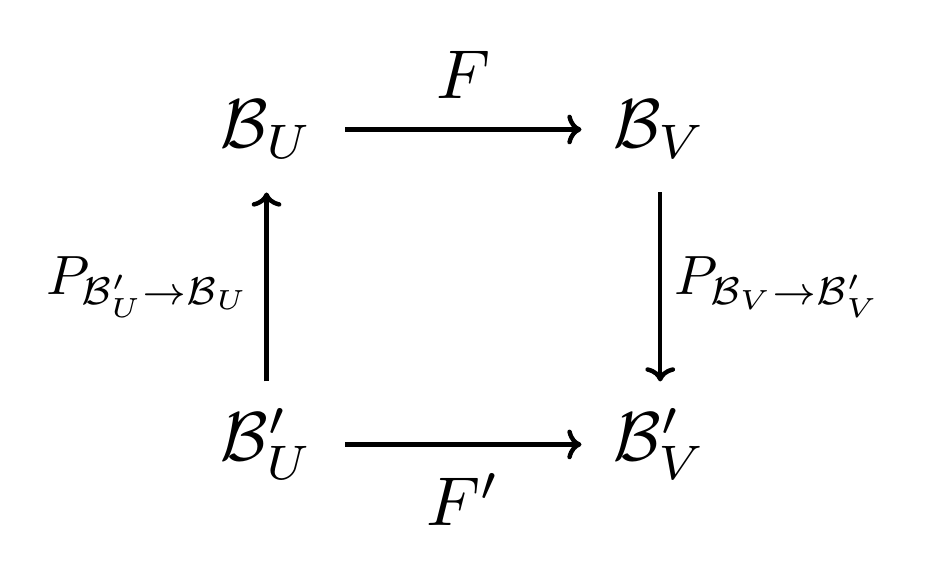
\begin{tikzpicture}
	\coordinate (U)  at (-2.5,+2);
	\coordinate (Ud) at (-2.5,-2);
	\coordinate (V)  at (+2.5,+2);
	\coordinate (Vd) at (+2.5,-2);
	
	\coordinate (F)  at (+0,+2.7);
	\coordinate (Fd) at (+0,-2.7);
	\coordinate (P1) at (-4,+0);
	\coordinate (P2) at (+4,+0);
	
	\node[black,scale=2.5] at (U)  {$\mathcal{B}_U$};
	\node[black,scale=2.5] at (Ud) {$\mathcal{B}'_U$};
	\node[black,scale=2.5] at (V)  {$\mathcal{B}_V$};
	\node[black,scale=2.5] at (Vd) {$\mathcal{B}'_V$};
	
	\node[black,scale=2.5] at (F)  {$F$};
	\node[black,scale=2.5] at (Fd) {$F'$};
	\node[black,scale=2] at (P1) {$P_{\mathcal{B}'_U\to\mathcal{B}_U}$};
	\node[black,scale=2] at (P2) {$P_{\mathcal{B}_V\to\mathcal{B}_V'}$};
	
	\draw[->,ultra thick] ($(U)+(1,0)$)--($(V)-(1,0)$);
	\draw[->,ultra thick] ($(Ud)+(1,0)$)--($(Vd)-(1,0)$);
	\draw[->,ultra thick] ($(Ud)+(0,0.8)$)--($(U)-(0,0.8)$);
	\draw[->,ultra thick] ($(V)-(0,0.8)$)--($(Vd)+(0,0.8)$);
\end{tikzpicture}
\end{figure}
To read this schematic, consider that the arrow for $F'$ has the same input and output as following the other three arrows to go up, then right (through $F$) then down again. This ordered path is the matrix multiplication given above.
}

		\chapter{Eigenvalues and Eigenvectors} \label{ch:eigens}


\definition{Eigenvalues and eigenvectors of a linear map}{
Consider an endomorphism $f:V \to V$ and a vector $\mathbf{v}\in V$. We call a number $\lambda \neq 0$ an eigenvalue of $f$ if there exists a non-zero vector $\mathbf{v}$ satisfying the relation
\begin{align*}
f(\mathbf{v}) = \lambda \mathbf{v}.
\end{align*}
We say that $\mathbf{v}$ is an eigenvector of $f$ \textit{corresponding} or \textit{associated} to the eigenvalue $\lambda$.
}


\definition{Eigenvectors and eigenvalues of a matrix}{
For a square matrix $A$, an eigenvector of $A$ is a non-zero vector, $\mathbf{v}$, that satisfies the matrix equation
\begin{align*}
A\mathbf{v} = \lambda \mathbf{v}
\end{align*}
where $\lambda$ is called an eigenvalue of $A$. We say that $\mathbf{v}$ is an eigenvector of $A$ \textit{corresponding} or \textit{associated} to the eigenvalue $\lambda$.
}


\definition{Characteristic polynomial of a matrix}{
For a square matrix $A$, the \textit{characteristic polynomial} is the given by
\begin{align*}
P(\lambda) = \det ( A - \lambda I)
\end{align*}
where $I$ is the identity matrix with the same size as $A$ and $\lambda$ is the variable of the polynomial. The degree of this polynomial is always the same as the size of the matrix $A$.
}


\definition{Eigenspectrum}{
The eigenvalues of a square matrix $A$ are roots of the characteristic polynomial of $A$. That is, eigenvalues are solutions of
\begin{align*}
 \det ( A - \lambda I) = 0.
\end{align*} 
There can be multiple distinct eigenvalues of $A$, and are conventionally denoted $\lambda_1$, $\lambda_2$, \dots etc. The set of these eigenvalues, $\{\lambda_1, \, \lambda_2, \dots \}$, is called the \textit{eigenspectrum} of $A$.
}


\definition{Eigenspace}{
For any eigenvalue $\lambda_k$ of an $n \times n$ matrix $A$, the eigenspace corresponding to $\lambda_k$, denoted $E_{\lambda_k}$, is the set of all eigenvectors corresponding to $\lambda_k$. This can be written as the set of linear combinations of linearly independent eigenvectors corresponding to $\lambda_k$:
\begin{gather*}
E_{\lambda_k} = \{ \alpha_1 \mathbf{v}_1 + \cdots + \alpha_m \mathbf{v}_m \, | \, \forall j \, A \mathbf{v}_j = \lambda_k \mathbf{v}_j, \, \alpha_j \in \mathbb{R} \} = \text{SPAN}(\mathbf{v}_1, \cdots, \mathbf{v}_m) \\
\text{for maximum number of eigenvectors such that} \\
\alpha_1 \mathbf{v}_1 + \cdots + \alpha_m \mathbf{v}_m = \mathbf{0} \implies  \alpha_1 =  \alpha_2 = \cdots = \alpha_m = 0.
\end{gather*}
As the set $\{\mathbf{v}_1, \cdots, \mathbf{v}_m\}$ generates $E_{\lambda_k}$ and the vectors are linearly independent, the set forms a basis and therefore gives the dimension $E_{\lambda_k}$.

The eigenspace can also be written like a \textit{kernel}
\begin{align*}
E_{\lambda_k} = \{ \mathbf{v} \in \mathbb{R}^n \, | \, \left( A - \lambda_k I \right) \mathbf{v}= \mathbf{0} \}.
\end{align*}
}


\definition{Algebraic and geometric multiplicity of an eigenvalue}{
For an $n \times n$ matrix with characteristic polynomial
\begin{align*}
P(\lambda) = C(\lambda - \lambda_1)^{m_1} \times \cdot \times (\lambda - \lambda_k)^{m_k}\times  \cdot \times (\lambda - \lambda_p)^{m_p}
\end{align*}
for some constant $C$. There can be up to $n$ distinct eigenvalues ($p \leq n$). The exponent $m_k$ is called the \textit{algebraic} multiplicity of the eigenvalue $\lambda_k$. The \textit{dimension} of the eigenspace corresponding to $\lambda_k$ is its \textit{geometric} multiplicity.
}



\definition{Eigenbasis}{
Consider a square matrix $A$ of size $n$. If the dimensions of its eigenspaces add up to $n$, then there exist $n$ linearly independent eigenvectors of $A$. These eigenvectors form a basis of $\mathbb{R}^n$ called an \textit{eigenbasis}.
}


\definition{Similar matrices}{
Two matrices $A$ and $B$ are similar if there exists an invertible matrix $P$ such that
\begin{align*}
B = P A P^{-1}.
\end{align*}
}


\definition{Diagonalizable linear map}{
Let $f:V\to V$ be an endomorphism. $f$ is called \textit{diagonalizable} if there exists a basis, $\mathcal{B}$, of $V$ such that the matrix representation of $f$ in $\mathcal{B}$ is diagonal:
\begin{align*}
(\mathcal{M}(f,\mathcal{B}))_{ij} = 0 \quad \text{whenever } \, i \neq j.
\end{align*}
}

\definition{Diagonalizable matrix}{
A square matrix $A$ is \textit{diagonalizable} if and only if there exists an invertible matrix $P$ and diagonal matrix $D$ such that
\begin{align*}
A = P D P^{-1}.
\end{align*}
Alternative: A square matrix $A$ is \textit{diagonalizable} if and only if it is \textit{similar} to a diagonal matrix $D$. 
}

\definition{Eigenvalue diagonalization}{
For a diagonalizable matrix $A$ of size $n$, we can sometimes find a diagonal matrix consisting of the eigenvalues of $A$, $\lambda_1, \, \dots, \, \lambda_n$. In this case we can write
\begin{align*}
A = P D P^{-1}
\end{align*}
where $P$ consists of eigenvectors of $A$ as columns. The matrix $P$ is the transition matrix from the eigenbasis, $\mathcal{E}$, to the canonical basis of $\mathbb{R}^n$: $P_{\mathcal{E}\to \mathcal{C}_n}$.
}

		\chapter{Inner product spaces} \label{ch:innerproducts}




\definition{Inner product}{
An inner product is a mapping that takes any two vectors of a vector space, $V$, to a scalar, $f:~V\times~V~\to~\mathbb{R}$ but often denoted with angle brackets $f(\mathbf{u},\mathbf{v})=\langle \mathbf{u},\mathbf{v} \rangle$, satisfying the following properties:
\begin{align*}
& \forall \, \mathbf{u},\, \mathbf{v}, \, \mathbf{w} \in V \quad \text{and} \quad  \forall \, k \in \mathbb{R} & \\
(IP1) & \quad \langle \mathbf{u},\mathbf{v} \rangle = \langle \mathbf{v},\mathbf{u} \rangle & (\text{commutativity}) \\
%
(IP2) & \quad \langle \mathbf{u},\mathbf{v}+\mathbf{w} \rangle = \langle \mathbf{u},\mathbf{v} \rangle + \langle \mathbf{u},\mathbf{w} \rangle & (\text{linearity over vector addition}) \\
%
(IP3) & \quad \langle k\mathbf{u},\mathbf{v} \rangle = k\langle \mathbf{u},\mathbf{v} \rangle & (\text{linearity over scalar multiplication}) \\
%
(IP4) & \quad \langle \mathbf{u},\mathbf{u} \rangle \geq 0 & (\text{positive definite})
\end{align*}
}

\definition{Euclidean dot product}{
The \textit{Euclidean dot product} is the canonical inner product defined on the vector space of real $n$-tuples, $\mathbb{R}^n$. Given two vectors $\mathbf{u}=(u_1, \dots, u_n)$ and $\mathbf{v}=(v_1, \dots, v_n)$, their dot product is defined by
\begin{align*}
\mathbf{u} \cdot \mathbf{v} = u_1 v_1 + \cdots + u_n v_n = \sum_{i=1}^n u_i v_i.
\end{align*}
}

\definition{Inner product of functions}{
Let $\mathcal{C}([a,b])$ be the vector space of real functions that are continuous on the interval $[a,b]$. We can define an inner product on any functions $f,g \in \mathcal{C}([a,b])$
\begin{align*}
\langle f,g \rangle = \int_a^b f(x)g(x) dx.
\end{align*}
You should verify that this definition satisfies the 4 properties of inner products.
}

\definition{Inner product space}{
An \textit{inner product space} is a vector space and a definition of an inner product considered as a pair $(V,\langle,\rangle)$. We say that $V$ is \textit{equipped} with the inner product.
}

\definition{Euclidean inner product space}{
A \textit{Euclidean inner product space} is the vector space of real $n$-tuples equipped with the euclidean dot product: $(\mathbb{R}^n, \cdot)$.
}

\definition{Orthogonal vectors}{
Two vectors $\mathbf{u}$ and $\mathbf{v}$ of an inner product space $(V,\langle,\rangle)$ are \textit{orthogonal} if and only if their inner product is zero: $\langle \mathbf{u},\mathbf{v} \rangle = 0$.
}

\definition{Norm}{
A vector $\mathbf{v}$ in an inner product space $(V,\langle,\rangle)$ has \textit{norm}
\begin{align*}
\lVert \mathbf{v} \rVert = \sqrt{\langle \mathbf{v},\mathbf{v} \rangle}.
\end{align*}
The Euclidean norm is therefore
\begin{align*}
\lVert (v_1, \dots, v_n) \rVert = \sqrt{v_1^2 + \cdots + v_n^2}.
\end{align*}
If a vector has norm equal to 1 we say it is a \textit{unit vector} or has \textit{unit length}. If we divide a vector by its norm we say that is has been \textit{normalised}.
}

\definition{To normalise a vector}{
Consider a vector $\mathbf{v}$ in an inner product space $(V,\langle,\rangle)$. We say we ``normalise'' this vector by dividing it by its norm. That is, $\mathbf{v}'$ is the normalised $\mathbf{v}$ if
\begin{align*}
\mathbf{v}' = \frac{\mathbf{v}}{\lVert \mathbf{v} \rVert}.
\end{align*}
}

\noindent When we normalise a vector we guarantee that it has length 1:
\begin{align*}
\lVert  \frac{\mathbf{v}}{\lVert \mathbf{v} \rVert} \rVert =  \frac{\lVert \mathbf{v} \rVert}{\lVert \mathbf{v} \rVert} = 1
\end{align*}


\definition{Orthonormal basis}{
An \textit{orthonormal basis} of an inner product space $(V,\langle,\rangle)$ is a set of vectors 
$\mathcal{B} = \{\mathbf{v}_1, \dots, \mathbf{v}_n\}$ each having norm of 1 and that are pairwise orthogonal:
\begin{align*}
\langle \mathbf{v}_i, \mathbf{v}_j \rangle 
=  
\begin{cases}
1 & \text{whenever } \, i = j, \\
0 & \text{whenever } \, i \neq j.
\end{cases}
\end{align*}
}

		\chapter{Orthogonal matrices} \label{ch:orthogonal}


\definition{Orthogonal matrix}{
A square matrix $A$ is orthogonal if and only if its inverse is its transpose. That is, if and only if $A A^T = A^T A = I$.
}

\definition{Properties of orthogonal matrices}{
If $A$ is an orthogonal matrix of size $n$, then
\begin{itemize}
	\item its columns are pair-wise orthogonal,
	\item its columns are unit length,
	\item its columns (considered as $n$-tuples) form an orthonormal basis of $\mathbb{R}^n$,
	\item its rows (considered as $n$-tuples) form an orthonormal basis of $\mathbb{R}^n$,
	\item it has determinant $\pm 1$.
\end{itemize}
}


\definition{Orthogonally diagonalizable matrix}{
A square matrix $A$ is orthogonally diagonalizable if there exists a diagonal matrix $D$ and orthogonal matrix $Q$ such that
\begin{align*}
A = Q D Q^T.
\end{align*}
}


\definition{Quadratic form}{
Let $A$ be an $n \times n$ matrix and $\mathbf{v} \in \mathbf{R}^n$ \textit{considered as a column}. Then a quadratic form is a multiplication of the form $\mathbf{v}^T A  \mathbf{v}$ resulting in a real number.
}

\definition{Definite matrix}{
Let $A$ be an $n \times n$ symmetric real matrix. By considering the sign of quadratic forms with $A$ we can define several cases. $A$ is
\begin{itemize}
 \item \textit{positive definite} if an only if $\mathbf{v}^T A \mathbf{v} > 0$ for every $\mathbf{v}\in\mathbb{R}^n$,
 \item \textit{positive semi-definite} if an only if $\mathbf{v}^T A \mathbf{v} \geq 0$ for every $\mathbf{v}\in\mathbb{R}^n$,
 \item \textit{negative definite} if an only if $\mathbf{v}^T A \mathbf{v} < 0$ for every $\mathbf{v}\in\mathbb{R}^n$,
 \item \textit{negative semi-definite} if an only if $\mathbf{v}^T A \mathbf{v} \leq 0$ for every $\mathbf{v}\in\mathbb{R}^n$.
\end{itemize}
If the matrix does not satisfy any of these (e.g. if we can find a positive and a negative quadratic form) then the matrix is called \textit{indefinite}.
}


\definition{Eigenvalues of a definite matrix}{
Let $A$ be an $n \times n$ symmetric real matrix. Then all eigenvalues of $A$ are real numbers. Furthermore, $A$ is
\begin{itemize}
 \item \textit{positive definite} if an only if every eigenvalue is strictly positive,
 \item \textit{positive semi-definite} if an only if every eigenvalue is non-negative,
 \item \textit{negative definite} if an only if every eigenvalue is strictly negative,
 \item \textit{negative semi-definite} if an only if every eigenvalue is strictly non-positive.
\end{itemize}
}


	\else 
		\ifnum \version = 0
		\thispagestyle{empty}
\begin{titlepage}

\newcommand{\HRule}{\rule{\linewidth}{0.5mm}} % Defines a new command for the horizontal lines, change thickness here

\center % Center everything on the page
 
%----------------------------------------------------------------------------------------
%	HEADING SECTIONS
%----------------------------------------------------------------------------------------

%\textsc{\LARGE Macquarie University}\\[1.5cm] % Name of your university/college
%\textsc{\Large Honours Thesis}\\[0.5cm] % Major heading such as course name



%----------------------------------------------------------------------------------------
%	DATE SECTION
%----------------------------------------------------------------------------------------
%\includegraphics[width=1.0\textwidth]{Front2.jpg}\\[1.0cm]

%----------------------------------------------------------------------------------------
%	TITLE SECTION
%----------------------------------------------------------------------------------------

\HRule \\[0.4cm]
{ \huge \bfseries Incomplete Notes On}\\[0.4cm] % Title of your document
{ \huge \bfseries Numerical Methods} % Title of your document
\HRule \\[0.2cm]
 
%----------------------------------------------------------------------------------------
%	AUTHOR SECTION
%----------------------------------------------------------------------------------------



\begin{minipage}{0.4\textwidth}
\begin{flushleft} \large
\centering Andrew Lehmann \\
\centering \today \\
\end{flushleft}
\end{minipage}

\vfill

\begin{figure}[H]
\includegraphics[width=\textwidth]{figures/ch3_lagrange_total.pdf}
\end{figure}

\vfill % Fill the rest of the page with whitespace

\begin{center}
Typeset in \LaTeXe.
\end{center}
\end{titlepage}

	
		\addcontentsline{toc}{chapter}{\bf Contents}
		\tableofcontents

		\clearpage

		% List of Definitions and Theorems
		%\listoftheorems[ignoreall]
		\renewcommand{\listtheoremname}{List of Definitions}
		\listoftheorems[ignoreall,show=definitionnew]

		\clearpage
		\pagenumbering{arabic}
		\chapter{Euclidean Vectors} \label{ch:euclid}


\definition{Euclidean vector or tuple}{
A Euclidean vector is a list of $n$ real numbers, also called an $n$-tuple. We write this list in parentheses, for example $(1,3,-2, \dots, 0)$, and we say that this object belongs to $\mathbb{R}^n$. An arbitrary tuple can be written $\mathbf{v}=(v_1,v_2,\cdots,v_n)$ where the \textit{components} $v_i \in \mathbb{R}$ for any index $i$.
}


\definition{Tuple addition}{
Euclidean vectors are added to each other component by component. In symbols
\begin{align*}
(a_1, a_2, \dots, a_n) + (b_1, b_2, \dots, b_n) = (a_1+b_1, a_2+b_2, \dots, a_n + b_n).
\end{align*}
\textit{Note}: this means you can only add two tuples together \textit{of the same size}. It makes no sense to add a 3-tuple to a 5-tuple.
}


\definition{Scalar multiplication}{
Let $c\in\mathbb{R}$, called a scalar quantity, and $\mathbf{v} \in \mathbb{R}^n$ with components $v_i$. Then the \textit{scalar multiplication} $c\mathbf{v}$ gives a vector $\mathbf{w}$ with components $w_i = c v_i$ for every index $i$. In tuple form
\begin{align*}
c(v_1,v_2,\dots,v_n) = (cv_1,cv_2,\dots,cv_n).
\end{align*}
}


\definition{Canonical Euclidean unit vectors}{
The canonical Euclidean vectors in $\mathbb{R}^n$ are the $n$ vectors of the form
\begin{gather*}
\mathbf{e}_1 = (1,0,\dots,0) \\
\mathbf{e}_2 = (0,1,\dots,0) \\
\vdots \\
\mathbf{e}_n = (0,0,\dots,1).
\end{gather*}
More compactly
\begin{align*}
\mathbf{e}_k = (\alpha_1, \alpha_2, \dots, \alpha_n) \quad \text{where} \quad
\alpha_j=
\begin{cases}
1 & \text{for } j= k, \\
0 & \text{for } j\neq k.
\end{cases}
\end{align*}
}


\definition{Dot product}{
For two $n$-tuples $\mathbf{a}$ and $\mathbf{b}$, their \textit{dot product}, also called \textit{scalar} product and \textit{Euclidean inner} product, is the real number given by the addition of component by component multiplication
\begin{align*}
\mathbf{a}\cdot\mathbf{b} = a_1 b_1 + a_2 b_2 + \cdots + a_n b_n = \sum_{i=1}^n a_i b_i.
\end{align*}
}

\definition{Euclidean Norm}{
The norm of an $n$-tuple $\mathbf{v}$, denoted $\lVert \mathbf{v} \rVert$, is given by
\begin{align*}
\lVert \mathbf{v} \rVert = \sqrt{\mathbf{v}\cdot\mathbf{v}} = \sqrt{v_1^2 + v_2^2 + \cdots + v_2^2}.
\end{align*}
}

\definition{Orthogonal Euclidean vectors}{
Two vectors in $\mathbb{R}^n$ are orthogonal if and only if their dot product equals zero.
}

\definition{Displacement vector}{
Given two Euclidean vectors $\mathbf{a}$ and $\mathbf{b}$, the displacement vector pointing from $\mathbf{a}$ to $\mathbf{b}$ is given by $\mathbf{r}=\mathbf{b}-\mathbf{a}$ as pictured below. Of course we can also create the displacement vector in the other direction, from $\mathbf{b}$ to $\mathbf{a}$, given by $\mathbf{a}-\mathbf{b}$.
}


\definition{Vector form of a straight line}{
The set of vectors in $\mathbb{R}^n$ of the form $\mathbf{v} = \mathbf{a} + t \mathbf{r}$ for a parameter $t\in\mathbb{R}$ represents a straight line through the space $\mathbb{R}^n$. That is,
\begin{align*}
\{(x,y) \, | \, \forall x\in\mathbb{R} \, \text{and} \, y=mx+b  \} = \{ \mathbf{a} + t \mathbf{r} \, | \, \forall t\in\mathbb{R} \}
\end{align*}
where $\mathbf{a}$ is an arbitrary pair $(x,mx+b)$ and $\mathbf{r}$ is a displacement vector between any two distinct pairs $(x_1,mx_1+b)$ and $(x_2,mx_2+b)$.
}


		\chapter{Matrix Algebra} \label{ch:matrixalgebra}


\definition{Matrix}{
A matrix is a collection of numbers from a field $\mathbb{F}$ (e.g. rational numbers) usually represented by a rectangular array. For example, an $m \times n$ (said m by n) matrix $A$ with coefficients $a_{ij}\in\mathbb{F}$  would be represented by an array with $m$ rows and $n$ columns:
\begin{align*}
A = 
\begin{pmatrix}
a_{11} & a_{12} & a_{13} & \cdots & a_{1j} & \cdots & a_{1m} \\
a_{21} & a_{22} & a_{23} & \cdots & a_{2j} & \cdots & a_{2m} \\
a_{31} & a_{32} & a_{33} & \cdots & a_{3j} & \cdots & a_{3m} \\
\vdots & \vdots & \vdots & \ddots & \vdots & \ddots & \vdots \\
a_{i1} & a_{12} & a_{13} & \cdots & a_{ij} & \cdots & a_{im} \\
\vdots & \vdots & \vdots & \ddots & \vdots & \ddots & \vdots \\
a_{n1} & a_{n2} & a_{n3} & \cdots & a_{nj} & \cdots & a_{nm}
\end{pmatrix}
=
\left( a_{ij} \right)_{\substack{ 1 \leq i \leq m \\ 1 \leq j \leq n }}.
\end{align*}
Sometimes it is convenient to refer to the coefficients in the array like so: $a_{ij} = \left(A\right)_{ij}$.
}

\definition{Set of all $m \times n$ matrices}{
We write the set of all $m \times n$ matrices with coefficients in $\mathbb{F}$ as
\begin{align*}
\mathcal{M}_{m,n}(\mathbb{F})
\end{align*}
}

\definition{Matrix columns and rows}{
For a matrix $A\in\mathcal{M}_{m,n}(\mathbb{F})$ we denote its j$^{th}$ column and i$^{th}$ row
\begin{align*}
A^{(j)} =
\begin{pmatrix}
 a_{1j} \\
 a_{2j} \\
 a_{3j} \\
 \vdots \\
 a_{ij} \\
 \vdots \\
 a_{mj}
\end{pmatrix},
\qquad
A_{(i)} =
\begin{pmatrix}
a_{i1} & a_{12} & a_{13} & \cdots & a_{ij} & \cdots & a_{in}
\end{pmatrix}
\end{align*}
}

\definition{Transpose of a matrix}{
The transpose of an $m \times n$ matrix, $A$, is an $n \times m$ matrix, denoted $A^T$, with rows equal to the columns of $A$. That is, $\left(A^T\right)_{ij} = \left(A\right)_{ji}$ for all combinations of $i$ and $j$. 
}



\definition{Diagonal matrix}{
A square matrix $A$ is said to be diagonal if all its non-diagonal elements are zero, e.g. $(A)_{ij}=0$ whenever $i \neq j$.
}

\definition{Symmetric matrix}{
A matrix $A$ is symmetric if it is equal to its transpose, $A = A^T$.
}



\definition{Matrix addition}{
Matrix addition is done coefficient by coefficient, that is, for two matrices $A$ and $B$ we define the i,j$^{th}$ coefficient of the addition as the addition of the i,j$^{th}$ coefficients of each matrix: 
\begin{align*}
\left(A+B\right)_{ij} = \left(A\right)_{ij}+\left(B\right)_{ij}.
\end{align*}
}



\definition{Scalar multiplication}{
Given a number $k\in\mathbb{R}$ (called a scalar) and a matrix $A \in \mathcal{M}_{m,n}$, we define matrix scalar multiplication, $kA$, to be a matrix $B \in \mathcal{M}_{m,n}$ with coefficients given by:
\begin{align*}
b_{ij} = ka_{ij},
\end{align*}
that is, we multiply \textit{every coefficient} by the scalar.
} 


\definition{Zero matrix}{
The zero matrix of any shape is a matrix $M_0 \in\mathcal{M}_{m,n}$ consisting entirely of zeros as coefficients.
} 


\definition{Additive inverse}{
Given a matrix $A\in\mathcal{M}_{ij}$, its additive inverse is the same matrix multiplied by the scalar $-1$. We denote the additive inverse of $A$ as $-A$.
} 


\definition{Multiplication of a matrix by a column}{
Consider a matrix $A \in \mathcal{M}_{m,n}$ and a column $X \in \mathcal{M}_{n,1}$. We define the product $AX$ to result in the column $Y\in\mathcal{M}_{m,1}$ with coefficients
\begin{align*}
(Y)_i = a_{i1}x_1 + a_{i2}x_2 + \cdots + a_{im}x_m = \sum_{k=1}^m a_{ik} x_k 
\end{align*}
Visually
\begin{align*}
\begin{pmatrix}
y_{1} \\
y_{2} \\
\vdots \\
y_{n} 
\end{pmatrix}
%%%
%%%
%%%
&=
%%%
\begin{pmatrix}
a_{11} & a_{12} & \cdots & a_{1m} \\
a_{21} & a_{22} & \cdots & a_{2m} \\
\vdots & \vdots & \ddots & \vdots \\
a_{n1} & a_{n2} & \cdots & a_{nm}
\end{pmatrix}
\begin{pmatrix}
x_{1} \\
x_{2} \\
\vdots \\
x_{m} 
\end{pmatrix}
%%%
%%%
%%%
=
%%%
x_{1}
\begin{pmatrix}
a_{11} \\
a_{21} \\
\vdots \\
a_{n1} 
\end{pmatrix}
+
x_{2}
\begin{pmatrix}
a_{12} \\
a_{22} \\
\vdots \\
a_{n2} 
\end{pmatrix}
+ \cdots +
x_m
\begin{pmatrix}
a_{1m} \\
a_{2m} \\
\vdots \\
a_{nm} 
\end{pmatrix}
\\ \\
%%%
%%%
%%%
&\implies Y = x_{1}A^{(1)} + x_{2}A^{(2)} + \cdots + x_{m}A^{(m)}
\end{align*}
}

\definition{Rotation matrix - arbtirary angle anti-clockwise}{
By using a column $X\in\mathcal{M}_{2,1}$ to represent a Euclidean vector, the following matrix allows the operation of rotataion, anti-clockwise, of $X$ by an angle $\theta$:
\begin{align*}
R_\theta =
\begin{pmatrix} 
\cos\theta & -\sin\theta \\ 
\sin\theta &  \cos\theta  
\end{pmatrix}
\end{align*}
where the rotated vector is represented by a column $X'\in\mathcal{M}_{2,1}$ obtained by matrix multiplication $X' = R_\theta X$.
}


\definition{Multiplication of two matrices}{
Consider two matrices $A \in \mathcal{M}_{n,m}$ and $B \in \mathcal{M}_{m,q}$. We define the product $AB$ to be the matrix $C\in\mathcal{M}_{n,q}$ with coefficients
\begin{gather*}
c_{ij} = a_{i1}b_{1j} + a_{i2}b_{2j} + \cdots + a_{im}b_{mj} = \sum_{k=1}^m a_{ik} b_{kj} \\
%%%
%%%
%%%
\implies
\begin{pmatrix}
a_{11} & a_{12} & \cdots & a_{1m} \\
a_{21} & a_{22} & \cdots & a_{2m} \\
\vdots & \vdots & \ddots & \vdots \\
a_{n1} & a_{n2} & \cdots & a_{nm}
\end{pmatrix}
\begin{pmatrix}
b_{11} & b_{12} & \cdots & b_{1q} \\
b_{21} & b_{22} & \cdots & b_{2q} \\
\vdots & \vdots & \ddots & \vdots \\
b_{m1} & b_{m2} & \cdots & b_{mq}
\end{pmatrix} \\
%%%
%%%
%%%
=
\left(
b_{11}
\underbrace{
\begin{pmatrix}
a_{11} \\
a_{21} \\
\vdots \\
a_{n1} 
\end{pmatrix}
+ \cdots +
b_{m1}
\begin{pmatrix}
a_{1m} \\
a_{2m} \\
\vdots \\
a_{nm} 
\end{pmatrix}
}_{\text{\large first column}}
%%
\quad \cdots \quad 
%%
b_{1q}
\underbrace{
\begin{pmatrix}
a_{11} \\
a_{21} \\
\vdots \\
a_{n1} 
\end{pmatrix}
+ \cdots +
b_{mq}
\begin{pmatrix}
a_{1m} \\
a_{2m} \\
\vdots \\
a_{nm} 
\end{pmatrix}
}_{\text{\large n$^{th}$ column}}
\right)
\end{gather*}
Additionally, for the product
\begin{align*}
\underbrace{A}_{(\colorbox{Mahogany!20}{n},\colorbox{airforceblue!20}{m})} \underbrace{B}_{(\colorbox{airforceblue!20}{m},\colorbox{Mahogany!20}{q})}
\end{align*}
we will call the indices for the columns of $A$ and rows of $B$ the \textit{inner indices} (blue), whereas the indices for the rows of $A$ and columns of $B$ will be called the \textit{outer indices} (red).
}

\definition{Identity matrix}{
The $n$-dimensional identity matrix $I$ is a square matrix of size $n\times n$ with 1s along the diagonal and 0s elsewhere, that is, 
\begin{align*}
(I)_{ij}
=
\begin{cases}
1 & \text{whenever } \, i=j, \\
0 & \text{whenever } \, i \neq j.
\end{cases}
\end{align*}
}

\definition{Invertible matrix}{
A matrix $A$ is invertible if and only if there exists a matrix $B$ such that
\begin{align*}
A B = BA = I
\end{align*}
This matrix $B$ is called the inverse of $A$ and is denoted $A^{-1}$. As we have commutative matrices, $AB=BA$, recall that this can only happen if $A$ is square. So, only square matrices can have inverses.
}

\definition{Determinant of a 1 by 1 matrix}{
The determinant of any 1 by 1 matrix is given by its only coefficient:

\begin{align*}
\det \left( \begin{pmatrix} a \end{pmatrix}\right)  = a
\end{align*}
}


\definition{Submatrix}{
From a matrix $A$ we generate the \textit{submatrix} $A_{ij}$ by deleting the $ith$ row and $jth$ column:
\begin{align*}
\text{For} \, A =
\begin{pmatrix}
a_{1,1}   & \cdots & a_{1,j-1}   & a_{1,j}   & a_{1,j+1}   & \cdots & a_{1,n}   \\
\vdots    & \cdots & \vdots      & \vdots    & \vdots      & \cdots & \vdots    \\
a_{i-1,1} & \cdots & a_{i-1,j-1} & a_{i-1,j} & a_{i-1,j+1} & \cdots & a_{i-1,n} \\
a_{i,1}   & \cdots & a_{i,j-1}   & a_{i,j}   & a_{i,j+1}   & \cdots & a_{i,n}   \\
a_{i+1,1} & \cdots & a_{i+1,j-1} & a_{i+1,j} & a_{i+1,j+1} & \cdots & a_{i+1,n} \\
\vdots    & \cdots & \vdots      & \vdots    & \vdots      & \cdots & \vdots    \\
a_{m,1}   & \cdots & a_{m,j-1}   & a_{m,j}   & a_{m,j+1}   & \cdots & a_{m,n} 
\end{pmatrix} \\
\text{The submatrix} \, A_{ij} =
\begin{pmatrix}
a_{1,1}   & \cdots & a_{1,j-1}   & a_{1,j+1}   & \cdots & a_{1,n}   \\
\vdots    & \cdots & \vdots      & \vdots      & \cdots & \vdots    \\
a_{i-1,1} & \cdots & a_{i-1,j-1} & a_{i-1,j+1} & \cdots & a_{i-1,n} \\
a_{i+1,1} & \cdots & a_{i+1,j-1} & a_{i+1,j+1} & \cdots & a_{i+1,n} \\
\vdots    & \cdots & \vdots      & \vdots      & \cdots & \vdots    \\
a_{m,1}   & \cdots & a_{m,j-1}   & a_{m,j+1}   & \cdots & a_{m,n} 
\end{pmatrix}
\end{align*}
\textit{Note}: we generally have to specify in words that we create a submatrix. The notation $A_{ij}$ is a little ambiguous without being explicit. 
}


\definition{Determinant of an $n \times n$ matrix}{
For any square matrix $A\in\mathcal{M}_{n,n}$, its determinant is given by
\begin{align*}
\det(A) = \sum_{i=1}^n (-1)^{i+j} a_{ij} \det(A_{ij})
\end{align*}
where the $a_{ij}$ are coefficients of $A$, $A_{ij}$ is the $i,j^{th}$ submatrix of $A$ and for any $1\leq j \leq n$. We can also sum over the $j$ index for any $1\leq i \leq n$
\begin{align*}
\det(A) = \sum_{j=1}^n (-1)^{i+j} a_{ij} \det(A_{ij})
\end{align*}
and we will show that the answer is the same.
}

\definition{Cramer system}{
Suppose we have the following linear system of equations (with unknowns equal to equations)
\begin{align*}
\begin{cases}
a_{11} x_1  + a_{12} x_2 + \cdots + a_{1n} x_n = y_1 \\
a_{21} x_1  + a_{22} x_2 + \cdots + a_{2n} x_n = y_2 \\
\vdots \\
a_{n1} x_1  + a_{n2} x_2 + \cdots + a_{nn} x_n = y_n
\end{cases}
\qquad (S)
\end{align*}
with the associated matrix form
\begin{align*}
\underbrace{
\begin{pmatrix}
a_{11} & a_{12} & \cdots & a_{1n} \\
a_{21} & a_{22} & \cdots & a_{2n} \\
\vdots & \vdots & \ddots & \vdots \\
a_{n1} & a_{n2} & \cdots & a_{nn}
\end{pmatrix}}_A
%%
%%
\underbrace{
\begin{pmatrix}
x_{1} \\
x_{2} \\
\vdots \\
x_{n}
\end{pmatrix}}_X
%%
=
\underbrace{
\begin{pmatrix}
y_{1} \\
y_{2} \\
\vdots \\
y_{n}
\end{pmatrix}}_Y
\end{align*}
We say that $(S)$ is a Cramer system if $\det(A) \neq 0$.
}

\definition{Cofactor matrix}{
From a matrix $A$ we generate its cofactor matrix $C_A$ which has entries given by determinants of submatrices of $A$ with the same plus/minus pattern as in a determinant calculation. That is, the entries of $C_A$ are $c_{ij}=(-1)^{i+j} \det(A_{ij})$:
\begin{align*}
C_A =
\begin{pmatrix}
 |A_{11}| & -|A_{12}| &  |A_{13}| & \cdots   \\
-|A_{21}| &  |A_{22}| & -|A_{23}| & \cdots   \\
 |A_{31}| & -|A_{32}| &  |A_{33}| & \cdots   \\
 \vdots   &  \vdots   &  \vdots   & \ddots
\end{pmatrix}
\end{align*}
}


		\chapter{Vector Spaces} \label{ch:vectorspaces}


\definition{Vector space}{
A \textit{vector space over a field} $\mathbb{F}$ is a set, call it $V$, with elements called vectors supplied with definitions of two operations, \textit{vector addition} (VA) and \textit{scalar multiplication} (SM), that satisfy the following \textit{vector space axioms}:
\begin{align*}
& \forall \, \mathbf{u},\mathbf{v},\mathbf{w} \in V \quad \text{and} \quad \forall \, k,l \in \mathbb{F} \\
\text{(VA1)} & \quad \mathbf{u} + \mathbf{v} \in V  & (\text{closure under vector addition})\\
%
\text{(VA2)} & \quad (\mathbf{u} + \mathbf{v}) + \mathbf{w}  =\mathbf{u} + (\mathbf{v} + \mathbf{w} ) & (\text{associativity of vector addition})\\
%
\text{(VA3)} & \quad \exists \, \mathbf{0} \in V, \, \text{such that} \, \mathbf{u} + \mathbf{0} = \mathbf{0} + \mathbf{u} = \mathbf{u} & (\text{additive identity})\\
%
\text{(VA4)} & \quad \exists \, -\mathbf{u} \in V \, \text{such that} \, \mathbf{u} + (-\mathbf{u}) = \mathbf{0} & (\text{additive inverse})\\
%
\text{(VA5)} & \quad \mathbf{u} + \mathbf{v} = \mathbf{v} + \mathbf{u} & (\text{commutativity of vector addition})\\
%
\text{(SM1)} & \quad k\mathbf{u} \in V & (\text{closure under scalar multiplication})\\
%
\text{(SM2)} & \quad k(\mathbf{u}+\mathbf{v})=k\mathbf{u}+k\mathbf{v} & (\text{distributivity over vector addition})\\
%
\text{(SM3)} & \quad (k+l)\mathbf{u}=k\mathbf{u}+l\mathbf{u} & (\text{distributivity over field addition})\\
%
\text{(SM4)} & \quad k(l\mathbf{u})=(kl)\mathbf{u} & (\text{compatibility of scalar and field multiplication})\\
%
\text{(SM5)} & \quad 1\mathbf{u}=\mathbf{u} & (\text{multiplicative identity})
\end{align*}
}

\definition{Linear Combination}{
Let \{$\mathbf{v}_1$, \dots, $\mathbf{v}_n$\} be a set of vectors in a vector space $V$. A linear combination of these vectors is a new vector, $\mathbf{w}\in V$, of the form
\begin{align*}
\mathbf{w} = \alpha_1 \mathbf{v}_1 + \cdots + \alpha_n \mathbf{v}_n
\end{align*}
where the $\alpha_k$ are real numbers.
}


\definition{Vector subspace}{
Suppose that $V$ is a vector space and $W$ is a subset of $V$. We call $W$ a \textit{vector subspace} if it satisfies the vector space axioms for the same definition of vector addition and scalar multiplication defined for $V$.
}


\definition{Span}{
Let $\mathcal{B} = \{\mathbf{v}_1, \dots, \mathbf{v}_n\}$ be a set of vectors from a vector space $V$. The span of these vectors is the set of all linear combinations of those vectors:
\begin{align*}
\text{SPAN}(\mathcal{B})  = \text{SPAN} (\mathbf{v}_1, \dots, \mathbf{v}_n) = \left\{ \alpha_1 \mathbf{v}_1 + \cdots + \alpha_n \mathbf{v}_n \, | \, \forall \alpha_1, \dots, \alpha_n \in \mathbb{R}^n \right\}.
\end{align*}
This set forms a vector subspace of $V$. It is obviously non-empty because it at least contains the vectors of $\mathcal{B}$. It is also automatically closed under vector addition and scalar multiplication because those are exactly the operations we used to create all the vectors in the span! Therefore $\text{SPAN}(\mathcal{B})$ is a vector subspace of $V$.
}


\definition{Cartesian form of Euclidean vector sub spaces}{
Euclidean vector sub spaces can always be written as a set with some defining equations:
\begin{align*}
\left\{ (x_1,\dots,x_n) \in \mathbb{R}^n \, | \, \text{equations relating the } x_k \right\}.
\end{align*}
For example, the general form of planar vector subspaces of $\mathbb{R}^3$ is
\begin{align*}
V_P = \left\{ (x,y,z)\in \mathbb{R}^3 \, | \, ax + by + cz = 0\right\}
\end{align*}
where $a$, $b$ and $c$ are some given constants. This set is read aloud as ``all the triples $(x,y,z)$ such that $ax + by + cz = 0$''.
}


\definition{Sum of subspaces (sum space)}{
Suppose we have a vector space $V$ with vector subspaces $F$ and $G$. We define the \textbf{sum of subspaces} (or sum space) as a new set denoted
\begin{align*}
F + G = \left\{ \textbf{f} + \textbf{g} \, | \, \textbf{f}\in F, \, \textbf{g}\in G\right\}
\end{align*}

\noindent \textit{Note}: The sum space is a \textit{subset} of the parent vector space: $F+G \subset V$.
}


\definition{Direct sum}{
Let $F$ and $G$ be two vector subspaces of a vector space $V$ and let $E=F+G$ be the sum space. We say $E$ is a \textbf{direct sum} of $F$ and $G$ if each element of $E$ has a \textbf{unique} decomposition as a sum of vectors in $F$ and vectors in $G$. That is, for every $\textbf{v}\in E$, there exists unique vectors $\textbf{f}\in F$ and $\textbf{g}\in G$ such that $\textbf{v} = \textbf{f} + \textbf{g}$. We denote this direct sum with a new symbol
\begin{align*}
E = F \oplus G
\end{align*}
}


\definition{Complementary vector subspaces}{
Let $F$ and $G$ be two vector subspaces of $V$. $F$ and $G$ are called \textbf{complementary} if $V$ is a direct sum of $F$ and $G$. That is, if and only if
\begin{itemize}
\item $V = F+G$, and
\item $F \cap G = \{\textbf{0}_V \}$
\end{itemize}
}

\definition{Linear dependence}{
A set of vectors $\{\mathbf{v}_1, \dots, \mathbf{v}_n\}$ from a vector space $V$ is said to be \textit{linearly dependent} if there exists a set of constants $\{ \alpha_1, \dots, \alpha_n \}$ \textit{not all zero} such that
\begin{align*}
\alpha_1 \mathbf{v}_1 + \cdots + \alpha_n \mathbf{v}_n = \mathbf{0}_V.
\end{align*}
\textit{Note}: the right hand side of the equation is the \textit{zero vector}, not the real number $0$.
}

\definition{Linear independence}{
A set of vectors $\{\mathbf{v}_1, \dots, \mathbf{v}_n\}$ from $V$ is said to be \textit{linearly independent} if they are not linearly dependent. That is, the equation
\begin{align*}
\alpha_1 \mathbf{v}_1 + \cdots + \alpha_n \mathbf{v}_n =  \mathbf{0}_V.
\end{align*}
implies that the constants $\alpha_1, \dots, \alpha_n$ \textit{are all zero}.
}


\definition{Basis}{
A \textit{basis of a vector space} $V$ is a minimal set of vectors which spans the vector space. Formally, the set of vectors $\mathcal{B}=\{\mathbf{v}_1, \dots, \mathbf{v}_n\}$ in a vector space $V$ is a basis of $V$ if it is a set of linearly independent vectors and $\text{SPAN}(\mathbf{v}_1, \dots, \mathbf{v}_n) = V$. \textit{Note}: bases are not unique, but they always contain the same number of vectors.
}

\definition{Dimension}{
The \textit{dimension of a vector space} is the number of elements in a basis for that vector space.
}

\definition{Canonical basis of $\mathbb{R}^n$}{
The \textit{canonical basis} of the vector space of real $n$-tuples, $\mathbb{R}^n$, is the ordered set of $n$ $n$-tuples with $k^{th}$ element, $\mathbf{c}_k=(\alpha_1, \dots, \alpha_n)$ such that 
\begin{align*}
\alpha_j = 
\begin{cases} 
1 & \text{for } j= k, \\
0 & \text{for } j\neq k.
\end{cases}
\end{align*}
That is, as a set the canonical basis is
\begin{align*}
\mathcal{C}_n=\{ 
(1, 0, \dots, 0 ), \,
(0, 1, \dots, 0 ), \,
\dots, \,
\underbrace{(0, 0, \dots, 0, \overbrace{1}^{k^{th} \text{ place}}, 0, \dots, 0 )}_{k^{th} \text{ tuple}}, \,
\dots, \,
(0, 0, \dots, 1)
\}.
\end{align*}
}


\definition{Canonical basis of $\mathcal{P}_n$}{
The \textit{canonical basis} of the vector space of polynomials with degree up to $n$, $\mathcal{P}_n$, is the ordered set of $n$ polynomials with $k^{th}$ element, $\mathbf{c}_k= x^k$. That is, as a set the canonical basis is
\begin{align*}
\mathcal{C}_n=\{ 
1, \,
x, \,
x^2, \,
\dots, \,
x^n
\}.
\end{align*}
}

\definition{Coordinates of a vector}{
Let $\mathbf{v}$ be a vector in a vector space $V$. The coordinates of $\mathbf{v}$ \textit{with respect to a given basis} $\mathcal{B}$, denoted $\left[\mathbf{v}\right]_\mathcal{B}$, is a column of the unique set of coefficients in the linear combination of $\mathbf{v}$ in terms of the basis vectors.
}

		\chapter{Linear Maps} \label{ch:linearmaps}

\definition{Linear map}{
A mapping, $f$, from a vector space $V$ to a vector space $W$, denoted $f:V \to W$, is called a \textit{linear map} if it satisfies the following property:
\begin{align*}
& \forall \mathbf{u}, \, \mathbf{v} \in V, \, \forall \alpha,\beta \in \mathbb{R} \\
& f(\alpha\mathbf{u} + \beta\mathbf{v}) = \alpha f(\mathbf{u}) + \beta f(\mathbf{v}).
\end{align*}
We say that a linear map \textit{preserves linear combinations}.
}


\definition{Image}{
The \textit{image of a linear map} $f: V \to W$, denoted $\text{im}(f)$, is the set of all possible ``output'' vectors of the map:
\begin{align*}
\text{im}(f) = \{ \mathbf{w} \in W \,\, | \,\, \exists \mathbf{v}\in V\, f(\mathbf{v}) = \mathbf{w} \} \subseteq W.
\end{align*}
}


\definition{Rank}{
The \textit{rank of a linear map} is the dimension of its image: $\text{rank}(f)=\dim(\text{im}(f))$.
}


\definition{Kernel}{
The \textit{kernel of a linear map}  $f: V \to W$, denoted $\ker(f)$, is the set of vectors that $f$ maps to the zero vector, $\mathbf{0}_W$, of $W$. That is,
\begin{align*}
\ker(f) = \{\mathbf{v} \in V \,\, | \,\, f(\mathbf{v}) = \mathbf{0}_W \}.
\end{align*}
}


\definition{Nullity}{
The \textit{nullity of a linear map} is the dimension of its kernel: $\text{nullity}(f)=\dim(\ker(f))$.
}





\definition{Injectivity}{
Let $f:V\to W$ be a linear map. We say $f$ is injective if no two vectors of $V$ are mapped to the same vector of $W$. In symbols we have two equivalent expressions
\begin{gather*}
\forall \, \mathbf{x},\mathbf{y}\in V, \quad \left(f(\mathbf{x})=f(\mathbf{y}) \implies \mathbf{x}=\mathbf{y}\right) \\
%
\text{or} \\
%
\forall \, \mathbf{x},\mathbf{y}\in V, \quad \left( \mathbf{x} \neq \mathbf{y} \implies f(\mathbf{x}) \neq f(\mathbf{y})\right)  
\end{gather*}
}

\definition{Surjectivity}{
Let $f:V\to W$ be a linear map. We say that $f$ is surjective if every vector in the output space has a corresponding input vector. In symbols
\begin{align*}
\forall \, \mathbf{w} \in W \quad \exists \mathbf{v}\in V \, \text{such that} \, f(\mathbf{v})=\mathbf{w}.
\end{align*}
}

\definition{Categories of linear maps}{
Let $f:V\to W$ be a linear map.
\begin{itemize}
\item If $W=V$ we call $f$ an \textit{endomorphism}.
\item If $f$ is both injective and surjective then we say it is bijective and we call it an \textit{isomorphism}.
\item If $f$ is both an isomorphism and an endomorphism we call it an \textit{automorphism}.
\end{itemize}
}

\definition{Composition of linear maps}{
Composition of linear maps works exactly as you would expect if you remember the composition of regular functions. We must have a coherence between the output of one linear map and the input of another. So, two linear maps $f:A\to B$ and $g:U\to V$ can be composed as a well defined linear map $g\circ f$ (``$g$ of $f$'') if and only if the output space of $f$ is the input space of $g$: $U=B$. For any $\mathbf{u}\in A$ the composition is written
\begin{align*}
g\circ f: A \to V \quad \text{and} \quad (g\circ f)(\mathbf{u}) = g(f(\mathbf{u})).
\end{align*}
}



\definition{Matrix representation of a linear map}{
Let $f:V \to W$ be a linear map, $\mathcal{A}=\{\mathbf{a}_1,\dots,\mathbf{a}_n\}$ be a basis of $V$, $\mathcal{B}=\{\mathbf{b}_1,\dots,\mathbf{b}_m\}$ be a basis of $W$. Let $\mathbf{v}$ be any vector in $V$ and $\mathbf{w}=f(\mathbf{v})\in W$. Then the \textit{matrix representation} of $f$ in bases $\mathcal{A}$ and $\mathcal{B}$, defined by the unique $m\times n$ matrix, denoted $\mathcal{M}(f,\mathcal{A}\to\mathcal{B})$, which takes the coordinates of $\mathbf{v}$ to the coordinates of $\mathbf{w}$ in their respective bases:
\begin{align*}
\mathcal{M}(f,\mathcal{A}\to\mathcal{B})[\mathbf{v}]_\mathcal{A} = [\mathbf{w}]_\mathcal{B}.
\end{align*}
can be calculated by expressing the coordinates of the linear map acting on the basis vectors of the input space
\begin{align*}
\mathcal{M}(f,\mathcal{A}\to\mathcal{B})=
\begin{pmatrix}
| &  & | \\
[f(\mathbf{a}_1)]_\mathcal{B} & \dots & [f(\mathbf{a}_n)]_\mathcal{B}\\
| &  & | 
\end{pmatrix}
\end{align*}
where the vertical lines are reminders that the coordinates of the $f(\mathbf{a}_k)$ vectors are columns. We often shorten ``matrix representation of $f$'' to just ``matrix of $f$''. If the input and output vector spaces are the same, i.e. if $f$ is an endomorphism, we can use the same basis for both spaces and we may shorten the notation $\mathcal{M}(f,\mathcal{A}\to\mathcal{A}) = \mathcal{M}(f,\mathcal{A})$.
}


\definition{Transition matrix (change-of-basis matrix)}{
The \textit{transition matrix} changes the representation of the coordinates of a vector from one basis into another. Let $\mathcal{A}$ and $\mathcal{B}$ be two bases of the same vector space, $V$, and let $\mathbf{v} \in V$. The transition matrix from $\mathcal{A}$ to $\mathcal{B}$, denoted $P_{\mathcal{A}\to \mathcal{B}}$ is defined by the relation
\begin{align*}
P_{\mathcal{A}\to \mathcal{B}} [\mathbf{v}]_\mathcal{A} = [\mathbf{v}]_\mathcal{B}.
\end{align*}
If we let the bases $\mathcal{A}=\{\mathbf{a}_1,\dots,\mathbf{a}_n\}$ and $\mathcal{B}=\{\mathbf{b}_1,\dots,\mathbf{b}_m\}$ then the transition matrix can be calculated by
\begin{align*}
P_{\mathcal{A}\to\mathcal{B}} =
\begin{pmatrix}
| & | & & | \\
[\mathbf{a}_1]_\mathcal{B} & [\mathbf{a}_2]_\mathcal{B} & \dots & [\mathbf{a}_n]_\mathcal{B}\\
| & | & & | 
\end{pmatrix}
\end{align*}
where the vertical lines are reminders that the coordinates of the $A$ basis vectors are columns.
}


\definition{Changing the bases of a matrix representation}{
Let $f:U \to V$ be a linear map, $\mathcal{B}_U$ and $\mathcal{B}'_U$ be two bases of $U$, $\mathcal{B}_V$ and $\mathcal{B}'_V$ be two bases of $V$, and $F=\mathcal{M}(f,\mathcal{B}_U\to\mathcal{B}_V)$ be the matrix representation of $f$ from basis $\mathcal{B}_U$ to basis $\mathcal{B}_V$. 

\noindent Then $F'=\mathcal{M}(f,\mathcal{B}'_U\to\mathcal{B}'_V)$, the matrix representation of $f$ from basis $\mathcal{B}'_U$ to basis $\mathcal{B}'_V$, is given by
\begin{align*}
F' = P_{\mathcal{B}_V\to\mathcal{B}_V'} \, F \, P_{\mathcal{B}'_U\to\mathcal{B}_U}
\end{align*}

\noindent The following diagram may help visualise this relation
\begin{figure}[H]
\centering
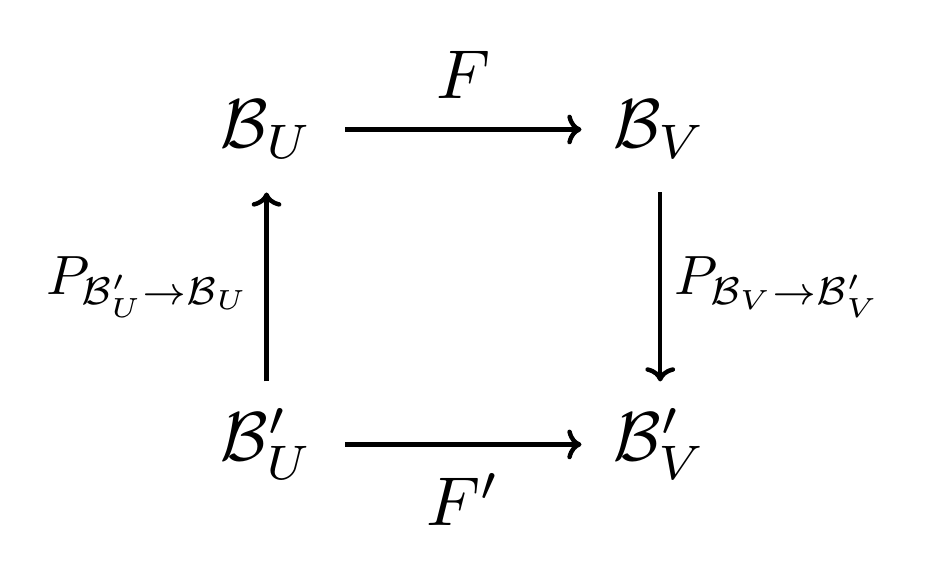
\begin{tikzpicture}
	\coordinate (U)  at (-2.5,+2);
	\coordinate (Ud) at (-2.5,-2);
	\coordinate (V)  at (+2.5,+2);
	\coordinate (Vd) at (+2.5,-2);
	
	\coordinate (F)  at (+0,+2.7);
	\coordinate (Fd) at (+0,-2.7);
	\coordinate (P1) at (-4,+0);
	\coordinate (P2) at (+4,+0);
	
	\node[black,scale=2.5] at (U)  {$\mathcal{B}_U$};
	\node[black,scale=2.5] at (Ud) {$\mathcal{B}'_U$};
	\node[black,scale=2.5] at (V)  {$\mathcal{B}_V$};
	\node[black,scale=2.5] at (Vd) {$\mathcal{B}'_V$};
	
	\node[black,scale=2.5] at (F)  {$F$};
	\node[black,scale=2.5] at (Fd) {$F'$};
	\node[black,scale=2] at (P1) {$P_{\mathcal{B}'_U\to\mathcal{B}_U}$};
	\node[black,scale=2] at (P2) {$P_{\mathcal{B}_V\to\mathcal{B}_V'}$};
	
	\draw[->,ultra thick] ($(U)+(1,0)$)--($(V)-(1,0)$);
	\draw[->,ultra thick] ($(Ud)+(1,0)$)--($(Vd)-(1,0)$);
	\draw[->,ultra thick] ($(Ud)+(0,0.8)$)--($(U)-(0,0.8)$);
	\draw[->,ultra thick] ($(V)-(0,0.8)$)--($(Vd)+(0,0.8)$);
\end{tikzpicture}
\end{figure}
To read this schematic, consider that the arrow for $F'$ has the same input and output as following the other three arrows to go up, then right (through $F$) then down again. This ordered path is the matrix multiplication given above.
}

		\chapter{Eigenvalues and Eigenvectors} \label{ch:eigens}


\definition{Eigenvalues and eigenvectors of a linear map}{
Consider an endomorphism $f:V \to V$ and a vector $\mathbf{v}\in V$. We call a number $\lambda \neq 0$ an eigenvalue of $f$ if there exists a non-zero vector $\mathbf{v}$ satisfying the relation
\begin{align*}
f(\mathbf{v}) = \lambda \mathbf{v}.
\end{align*}
We say that $\mathbf{v}$ is an eigenvector of $f$ \textit{corresponding} or \textit{associated} to the eigenvalue $\lambda$.
}


\definition{Eigenvectors and eigenvalues of a matrix}{
For a square matrix $A$, an eigenvector of $A$ is a non-zero vector, $\mathbf{v}$, that satisfies the matrix equation
\begin{align*}
A\mathbf{v} = \lambda \mathbf{v}
\end{align*}
where $\lambda$ is called an eigenvalue of $A$. We say that $\mathbf{v}$ is an eigenvector of $A$ \textit{corresponding} or \textit{associated} to the eigenvalue $\lambda$.
}


\definition{Characteristic polynomial of a matrix}{
For a square matrix $A$, the \textit{characteristic polynomial} is the given by
\begin{align*}
P(\lambda) = \det ( A - \lambda I)
\end{align*}
where $I$ is the identity matrix with the same size as $A$ and $\lambda$ is the variable of the polynomial. The degree of this polynomial is always the same as the size of the matrix $A$.
}


\definition{Eigenspectrum}{
The eigenvalues of a square matrix $A$ are roots of the characteristic polynomial of $A$. That is, eigenvalues are solutions of
\begin{align*}
 \det ( A - \lambda I) = 0.
\end{align*} 
There can be multiple distinct eigenvalues of $A$, and are conventionally denoted $\lambda_1$, $\lambda_2$, \dots etc. The set of these eigenvalues, $\{\lambda_1, \, \lambda_2, \dots \}$, is called the \textit{eigenspectrum} of $A$.
}


\definition{Eigenspace}{
For any eigenvalue $\lambda_k$ of an $n \times n$ matrix $A$, the eigenspace corresponding to $\lambda_k$, denoted $E_{\lambda_k}$, is the set of all eigenvectors corresponding to $\lambda_k$. This can be written as the set of linear combinations of linearly independent eigenvectors corresponding to $\lambda_k$:
\begin{gather*}
E_{\lambda_k} = \{ \alpha_1 \mathbf{v}_1 + \cdots + \alpha_m \mathbf{v}_m \, | \, \forall j \, A \mathbf{v}_j = \lambda_k \mathbf{v}_j, \, \alpha_j \in \mathbb{R} \} = \text{SPAN}(\mathbf{v}_1, \cdots, \mathbf{v}_m) \\
\text{for maximum number of eigenvectors such that} \\
\alpha_1 \mathbf{v}_1 + \cdots + \alpha_m \mathbf{v}_m = \mathbf{0} \implies  \alpha_1 =  \alpha_2 = \cdots = \alpha_m = 0.
\end{gather*}
As the set $\{\mathbf{v}_1, \cdots, \mathbf{v}_m\}$ generates $E_{\lambda_k}$ and the vectors are linearly independent, the set forms a basis and therefore gives the dimension $E_{\lambda_k}$.

The eigenspace can also be written like a \textit{kernel}
\begin{align*}
E_{\lambda_k} = \{ \mathbf{v} \in \mathbb{R}^n \, | \, \left( A - \lambda_k I \right) \mathbf{v}= \mathbf{0} \}.
\end{align*}
}


\definition{Algebraic and geometric multiplicity of an eigenvalue}{
For an $n \times n$ matrix with characteristic polynomial
\begin{align*}
P(\lambda) = C(\lambda - \lambda_1)^{m_1} \times \cdot \times (\lambda - \lambda_k)^{m_k}\times  \cdot \times (\lambda - \lambda_p)^{m_p}
\end{align*}
for some constant $C$. There can be up to $n$ distinct eigenvalues ($p \leq n$). The exponent $m_k$ is called the \textit{algebraic} multiplicity of the eigenvalue $\lambda_k$. The \textit{dimension} of the eigenspace corresponding to $\lambda_k$ is its \textit{geometric} multiplicity.
}



\definition{Eigenbasis}{
Consider a square matrix $A$ of size $n$. If the dimensions of its eigenspaces add up to $n$, then there exist $n$ linearly independent eigenvectors of $A$. These eigenvectors form a basis of $\mathbb{R}^n$ called an \textit{eigenbasis}.
}


\definition{Similar matrices}{
Two matrices $A$ and $B$ are similar if there exists an invertible matrix $P$ such that
\begin{align*}
B = P A P^{-1}.
\end{align*}
}


\definition{Diagonalizable linear map}{
Let $f:V\to V$ be an endomorphism. $f$ is called \textit{diagonalizable} if there exists a basis, $\mathcal{B}$, of $V$ such that the matrix representation of $f$ in $\mathcal{B}$ is diagonal:
\begin{align*}
(\mathcal{M}(f,\mathcal{B}))_{ij} = 0 \quad \text{whenever } \, i \neq j.
\end{align*}
}

\definition{Diagonalizable matrix}{
A square matrix $A$ is \textit{diagonalizable} if and only if there exists an invertible matrix $P$ and diagonal matrix $D$ such that
\begin{align*}
A = P D P^{-1}.
\end{align*}
Alternative: A square matrix $A$ is \textit{diagonalizable} if and only if it is \textit{similar} to a diagonal matrix $D$. 
}

\definition{Eigenvalue diagonalization}{
For a diagonalizable matrix $A$ of size $n$, we can sometimes find a diagonal matrix consisting of the eigenvalues of $A$, $\lambda_1, \, \dots, \, \lambda_n$. In this case we can write
\begin{align*}
A = P D P^{-1}
\end{align*}
where $P$ consists of eigenvectors of $A$ as columns. The matrix $P$ is the transition matrix from the eigenbasis, $\mathcal{E}$, to the canonical basis of $\mathbb{R}^n$: $P_{\mathcal{E}\to \mathcal{C}_n}$.
}

		\chapter{Inner product spaces} \label{ch:innerproducts}




\definition{Inner product}{
An inner product is a mapping that takes any two vectors of a vector space, $V$, to a scalar, $f:~V\times~V~\to~\mathbb{R}$ but often denoted with angle brackets $f(\mathbf{u},\mathbf{v})=\langle \mathbf{u},\mathbf{v} \rangle$, satisfying the following properties:
\begin{align*}
& \forall \, \mathbf{u},\, \mathbf{v}, \, \mathbf{w} \in V \quad \text{and} \quad  \forall \, k \in \mathbb{R} & \\
(IP1) & \quad \langle \mathbf{u},\mathbf{v} \rangle = \langle \mathbf{v},\mathbf{u} \rangle & (\text{commutativity}) \\
%
(IP2) & \quad \langle \mathbf{u},\mathbf{v}+\mathbf{w} \rangle = \langle \mathbf{u},\mathbf{v} \rangle + \langle \mathbf{u},\mathbf{w} \rangle & (\text{linearity over vector addition}) \\
%
(IP3) & \quad \langle k\mathbf{u},\mathbf{v} \rangle = k\langle \mathbf{u},\mathbf{v} \rangle & (\text{linearity over scalar multiplication}) \\
%
(IP4) & \quad \langle \mathbf{u},\mathbf{u} \rangle \geq 0 & (\text{positive definite})
\end{align*}
}

\definition{Euclidean dot product}{
The \textit{Euclidean dot product} is the canonical inner product defined on the vector space of real $n$-tuples, $\mathbb{R}^n$. Given two vectors $\mathbf{u}=(u_1, \dots, u_n)$ and $\mathbf{v}=(v_1, \dots, v_n)$, their dot product is defined by
\begin{align*}
\mathbf{u} \cdot \mathbf{v} = u_1 v_1 + \cdots + u_n v_n = \sum_{i=1}^n u_i v_i.
\end{align*}
}

\definition{Inner product of functions}{
Let $\mathcal{C}([a,b])$ be the vector space of real functions that are continuous on the interval $[a,b]$. We can define an inner product on any functions $f,g \in \mathcal{C}([a,b])$
\begin{align*}
\langle f,g \rangle = \int_a^b f(x)g(x) dx.
\end{align*}
You should verify that this definition satisfies the 4 properties of inner products.
}

\definition{Inner product space}{
An \textit{inner product space} is a vector space and a definition of an inner product considered as a pair $(V,\langle,\rangle)$. We say that $V$ is \textit{equipped} with the inner product.
}

\definition{Euclidean inner product space}{
A \textit{Euclidean inner product space} is the vector space of real $n$-tuples equipped with the euclidean dot product: $(\mathbb{R}^n, \cdot)$.
}

\definition{Orthogonal vectors}{
Two vectors $\mathbf{u}$ and $\mathbf{v}$ of an inner product space $(V,\langle,\rangle)$ are \textit{orthogonal} if and only if their inner product is zero: $\langle \mathbf{u},\mathbf{v} \rangle = 0$.
}

\definition{Norm}{
A vector $\mathbf{v}$ in an inner product space $(V,\langle,\rangle)$ has \textit{norm}
\begin{align*}
\lVert \mathbf{v} \rVert = \sqrt{\langle \mathbf{v},\mathbf{v} \rangle}.
\end{align*}
The Euclidean norm is therefore
\begin{align*}
\lVert (v_1, \dots, v_n) \rVert = \sqrt{v_1^2 + \cdots + v_n^2}.
\end{align*}
If a vector has norm equal to 1 we say it is a \textit{unit vector} or has \textit{unit length}. If we divide a vector by its norm we say that is has been \textit{normalised}.
}

\definition{To normalise a vector}{
Consider a vector $\mathbf{v}$ in an inner product space $(V,\langle,\rangle)$. We say we ``normalise'' this vector by dividing it by its norm. That is, $\mathbf{v}'$ is the normalised $\mathbf{v}$ if
\begin{align*}
\mathbf{v}' = \frac{\mathbf{v}}{\lVert \mathbf{v} \rVert}.
\end{align*}
}

\noindent When we normalise a vector we guarantee that it has length 1:
\begin{align*}
\lVert  \frac{\mathbf{v}}{\lVert \mathbf{v} \rVert} \rVert =  \frac{\lVert \mathbf{v} \rVert}{\lVert \mathbf{v} \rVert} = 1
\end{align*}


\definition{Orthonormal basis}{
An \textit{orthonormal basis} of an inner product space $(V,\langle,\rangle)$ is a set of vectors 
$\mathcal{B} = \{\mathbf{v}_1, \dots, \mathbf{v}_n\}$ each having norm of 1 and that are pairwise orthogonal:
\begin{align*}
\langle \mathbf{v}_i, \mathbf{v}_j \rangle 
=  
\begin{cases}
1 & \text{whenever } \, i = j, \\
0 & \text{whenever } \, i \neq j.
\end{cases}
\end{align*}
}

		\chapter{Orthogonal matrices} \label{ch:orthogonal}


\definition{Orthogonal matrix}{
A square matrix $A$ is orthogonal if and only if its inverse is its transpose. That is, if and only if $A A^T = A^T A = I$.
}

\definition{Properties of orthogonal matrices}{
If $A$ is an orthogonal matrix of size $n$, then
\begin{itemize}
	\item its columns are pair-wise orthogonal,
	\item its columns are unit length,
	\item its columns (considered as $n$-tuples) form an orthonormal basis of $\mathbb{R}^n$,
	\item its rows (considered as $n$-tuples) form an orthonormal basis of $\mathbb{R}^n$,
	\item it has determinant $\pm 1$.
\end{itemize}
}


\definition{Orthogonally diagonalizable matrix}{
A square matrix $A$ is orthogonally diagonalizable if there exists a diagonal matrix $D$ and orthogonal matrix $Q$ such that
\begin{align*}
A = Q D Q^T.
\end{align*}
}


\definition{Quadratic form}{
Let $A$ be an $n \times n$ matrix and $\mathbf{v} \in \mathbf{R}^n$ \textit{considered as a column}. Then a quadratic form is a multiplication of the form $\mathbf{v}^T A  \mathbf{v}$ resulting in a real number.
}

\definition{Definite matrix}{
Let $A$ be an $n \times n$ symmetric real matrix. By considering the sign of quadratic forms with $A$ we can define several cases. $A$ is
\begin{itemize}
 \item \textit{positive definite} if an only if $\mathbf{v}^T A \mathbf{v} > 0$ for every $\mathbf{v}\in\mathbb{R}^n$,
 \item \textit{positive semi-definite} if an only if $\mathbf{v}^T A \mathbf{v} \geq 0$ for every $\mathbf{v}\in\mathbb{R}^n$,
 \item \textit{negative definite} if an only if $\mathbf{v}^T A \mathbf{v} < 0$ for every $\mathbf{v}\in\mathbb{R}^n$,
 \item \textit{negative semi-definite} if an only if $\mathbf{v}^T A \mathbf{v} \leq 0$ for every $\mathbf{v}\in\mathbb{R}^n$.
\end{itemize}
If the matrix does not satisfy any of these (e.g. if we can find a positive and a negative quadratic form) then the matrix is called \textit{indefinite}.
}


\definition{Eigenvalues of a definite matrix}{
Let $A$ be an $n \times n$ symmetric real matrix. Then all eigenvalues of $A$ are real numbers. Furthermore, $A$ is
\begin{itemize}
 \item \textit{positive definite} if an only if every eigenvalue is strictly positive,
 \item \textit{positive semi-definite} if an only if every eigenvalue is non-negative,
 \item \textit{negative definite} if an only if every eigenvalue is strictly negative,
 \item \textit{negative semi-definite} if an only if every eigenvalue is strictly non-positive.
\end{itemize}
}


		\input{Defs_ComplexNumbers.tex}
		\input{Defs_QuantumMechanics.tex}
		\fi
	\fi
\fi
\onehalfspacing





\end{document}